\documentclass[11pt,a4paper]{article}
\usepackage{microtype}
\usepackage[margin=2.5cm]{geometry}
\usepackage{amsmath,amssymb,amsthm,mathtools}
\usepackage{booktabs,array,enumitem}
\usepackage{xcolor}
\usepackage{caption}
\usepackage{tikz}
\usetikzlibrary{arrows.meta,positioning,shapes.geometric,shapes.multipart,calc,fit,decorations.pathreplacing,backgrounds,matrix}
\usepackage{pgfplots}
\usepgfplotslibrary{groupplots}
\pgfplotsset{compat=1.16}
\usepackage{listings}
\usepackage[hidelinks]{hyperref}
\usepackage[nameinlink]{cleveref}

% ---------- environments (no boxes: book style) ----------
\newcounter{exn}[section]
\renewcommand{\theexn}{\thesection.\arabic{exn}}
\newcounter{oexn}
\renewcommand{\theoexn}{O.\arabic{oexn}}
\newenvironment{plainenglish}{\par\smallskip}{\par\smallskip}
\newenvironment{formal}{\par\smallskip}{\par\smallskip}
\newenvironment{exbox}[1][]{\par\medskip\refstepcounter{exn}\noindent\textbf{Example~\theexn\if\relax\detokenize{#1}\relax\else\ (#1)\fi.}\ \ignorespaces}{\hfill$\triangleleft$\par\medskip}
\newenvironment{oexbox}[1][]{\par\medskip\refstepcounter{oexn}\noindent\textbf{Example~\theoexn\if\relax\detokenize{#1}\relax\else\ (#1)\fi.}\ \ignorespaces}{\hfill$\triangleleft$\par\medskip}
\newenvironment{warnbox}[1][]{\par\medskip\noindent\textbf{Warning\if\relax\detokenize{#1}\relax\else\ #1\fi.}\ \ignorespaces}{\par\medskip}
\newenvironment{exercisebox}{\par\medskip\noindent\textbf{Exercises}\par\nopagebreak\smallskip}{\par\medskip}

% ---------- theorems ----------
\theoremstyle{definition}
\newtheorem{definition}{Definition}[section]
\newtheorem{example}[definition]{Example}
\theoremstyle{plain}
\newtheorem{theorem}[definition]{Theorem}
\newtheorem{lemma}[definition]{Lemma}
\newtheorem{proposition}[definition]{Proposition}
\newtheorem{corollary}[definition]{Corollary}
\theoremstyle{remark}
\newtheorem{remark}[definition]{Remark}

% ---------- macros ----------
\newcommand{\Hash}{\mathsf{H}}
\newcommand{\negl}{\mathsf{negl}}
\newcommand{\Z}{\mathbb{Z}}
\newcommand{\F}{\mathbb{F}}
\newcommand{\G}{\mathbb{G}}
\newcommand{\sk}{\mathsf{sk}}
\newcommand{\pk}{\mathsf{pk}}
\newcommand{\KeyGen}{\mathsf{KeyGen}}
\newcommand{\Sign}{\mathsf{Sign}}
\newcommand{\Verify}{\mathsf{Verify}}
\newcommand{\concat}{\,\|\,}
\newcommand{\E}{\mathbb{E}}
\renewcommand{\Pr}{\mathrm{Pr}}
\newcommand{\Adv}{\mathcal{A}}
\newcommand{\ie}{\textit{i.e.}}
\newcommand{\eg}{\textit{e.g.}}

\lstset{basicstyle=\ttfamily\small,breaklines=true,frame=single,
  backgroundcolor=\color{black!3},keywordstyle=\color{blue!60!black}\bfseries,
  commentstyle=\color{green!40!black}\itshape,columns=fullflexible}
\lstdefinelanguage{Solidity}{
  keywords={contract,function,public,external,payable,mapping,uint,uint256,address,require,return,msg,returns,view,if,else,emit,event,pragma,solidity,private,internal},
  sensitive=true,comment=[l]{//},morecomment=[s]{/*}{*/},morestring=[b]"}

\tikzset{
  blk/.style={draw,rounded corners=2pt,minimum width=1.9cm,minimum height=1.0cm,fill=blue!8,align=center,font=\small},
  adv/.style={draw,rounded corners=2pt,minimum width=1.9cm,minimum height=1.0cm,fill=red!12,align=center,font=\small},
  node/.style={draw,circle,minimum size=0.9cm,font=\small,fill=white},
    net/.style={circle,draw,minimum size=0.95cm,inner sep=0pt,font=\scriptsize},
  nM/.style={net,fill=yellow!45,very thick},
  nF/.style={net,fill=blue!12},
  nL/.style={net,dashed,minimum size=0.8cm,fill=white},
  nW/.style={net,dotted,thick,minimum size=0.75cm,fill=orange!12},
  nB/.style={net,fill=red!30,very thick},
  h0/.style={net,fill=red!40,very thick}, h1/.style={net,fill=orange!40},
  h2/.style={net,fill=yellow!45}, h3/.style={net,fill=green!35},
  h2d/.style={h2,dashed,minimum size=0.8cm}, h3d/.style={h3,dashed,minimum size=0.8cm}, h2t/.style={h2,dotted,thick,minimum size=0.75cm},
  badge/.style={circle,fill=black,text=white,inner sep=1.2pt,font=\tiny\bfseries},
>={Stealth[length=2.2mm]}
}

\newcommand{\netlegend}{%
\node[nM,minimum size=0.5cm] at (0,0) {}; \node[anchor=west,font=\footnotesize] at (0.4,0) {full miner};
\node[nF,minimum size=0.5cm] at (3.3,0) {}; \node[anchor=west,font=\footnotesize] at (3.7,0) {full node (no mining)};
\node[nL,minimum size=0.5cm] at (7.6,0) {}; \node[anchor=west,font=\footnotesize] at (8.0,0) {light node};
\node[nW,minimum size=0.5cm] at (10.6,0) {}; \node[anchor=west,font=\footnotesize] at (11.0,0) {pool (light) miner};}

\title{\textbf{Blockchain: Cryptography, Consensus and Security}\\[2mm]
\large Lecture notes for MPhil Cryptography (3--4 hours)}
\author{Dr.\ Faisal Aslam\\ FAST NUCES, Lahore}
\date{\today}

\begin{document}
\maketitle
\tableofcontents
\newpage

%================================================================
\section*{Overview: How a Blockchain Works}
\addcontentsline{toc}{section}{Overview: How a Blockchain Works}
%================================================================
\small
\setlength{\parskip}{0.3em}
\setlength{\abovecaptionskip}{3pt}

\subsection*{O.1\quad Why a blockchain?}
Digital money can be copied, so someone must decide the order of payments and reject a second spend of the same coin. Traditionally a bank or another central authority keeps the ledger and everybody trusts it. A blockchain removes this single point of trust: many independent computers each keep a copy of the ledger and follow the same public rules, so that no single party can rewrite history or block payments.

\subsection*{O.2\quad Blocks and the chain}
The ledger is a chain of \emph{blocks}. Each block has a \textbf{header} and a \textbf{body}. The header of block $B_i$ stores the hash of the header of $B_{i-1}$, so the blocks are linked: changing any old block changes its hash and breaks every later link. A block's identifier is the hash of its header; the body is covered by the header through the Merkle root (Section~O.4).

\begin{figure}[htbp]
\centering
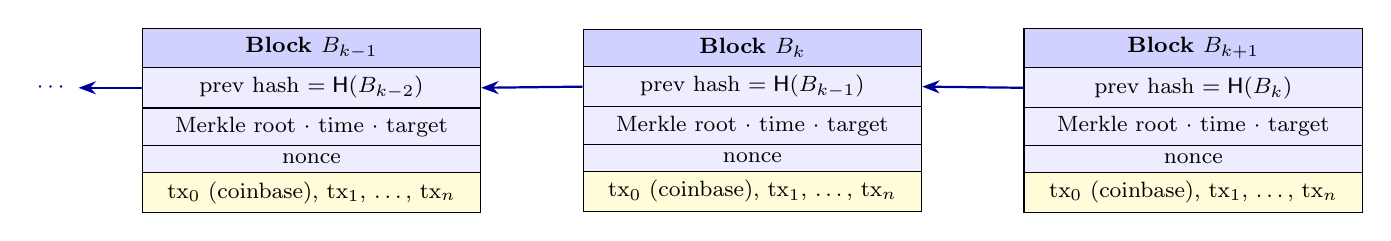
\begin{tikzpicture}[font=\footnotesize,
 bk/.style={draw,rectangle split,rectangle split parts=5,
   rectangle split part fill={blue!18,blue!7,blue!7,blue!7,yellow!15},
   minimum width=4.3cm,align=left,inner sep=3pt}]
\foreach \nm/\l/\x/\pl in {a/B_{k-1}/0/B_{k-2},b/B_{k}/5.6/B_{k-1},c/B_{k+1}/11.2/B_{k}}{
 \node[bk] (b\nm) at (\x,0) {\textbf{Block $\l$}
   \nodepart{two}prev hash $=\Hash(\pl)$
   \nodepart{three}Merkle root $\cdot$ time $\cdot$ target
   \nodepart{four}nonce
   \nodepart{five}tx$_0$ (coinbase), tx$_1$, \ldots, tx$_n$};
}
\draw[->,thick,blue!60!black] (bb.two west) -- (ba.two east);
\draw[->,thick,blue!60!black] (bc.two west) -- (bb.two east);
\draw[->,thick,blue!60!black] (ba.two west) -- ++(-0.8,0) node[left]{$\cdots$};
\end{tikzpicture}
\caption{A chain of blocks. The coloured rows form the header (the part that is hashed); the yellow row is the body, which the header commits to through the Merkle root. Each block stores the hash of its parent's header (the arrows are the hash pointers).}
\end{figure}

\begin{figure}[htbp]
\centering
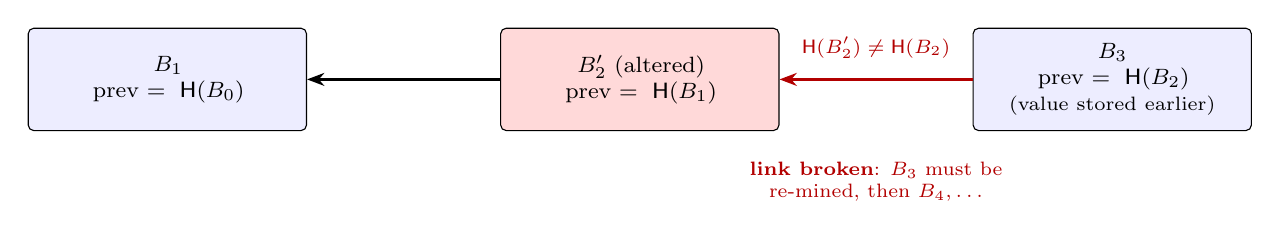
\begin{tikzpicture}[font=\footnotesize,
 bx/.style={draw,rounded corners=2pt,text width=3.3cm,minimum height=1.3cm,align=center,fill=blue!7}]
\node[bx] (a) at (0,0) {$B_1$\\ prev $=\Hash(B_0)$};
\node[bx,fill=red!15] (b) at (6,0) {$B_2'$ (altered)\\ prev $=\Hash(B_1)$};
\node[bx] (c) at (12,0) {$B_3$\\ prev $=\Hash(B_2)$\\ \scriptsize(value stored earlier)};
\draw[->,thick] (b)--(a);
\draw[->,thick,red!70!black] (c)--(b);
\node[red!70!black,align=center,font=\scriptsize] at (9,0.4) {$\Hash(B_2')\neq\Hash(B_2)$};
\node[red!70!black,align=center,font=\scriptsize] at (9,-1.3) {\textbf{link broken}: $B_3$ must be\\ re-mined, then $B_4,\ldots$};
\end{tikzpicture}
\caption{Tamper evidence. Altering a transaction in $B_2$ changes its Merkle root, hence the hash of its header, hence the pointer stored in $B_3$ is wrong. Repairing it means redoing the proof of work for $B_2'$, $B_3$ and every later block.}
\end{figure}

\begin{center}
\footnotesize\renewcommand{\arraystretch}{0.95}
\begin{tabular}{@{}p{3.6cm}p{11.8cm}@{}}
\toprule
\multicolumn{2}{@{}l}{\textbf{Header} (80 bytes in Bitcoin)}\\
\midrule
Version & which validation rules the block follows\\
Previous block hash & links the block to its parent and makes history tamper-evident\\
Merkle root & one hash that commits to all transactions in the body\\
Timestamp & approximate creation time; used to adjust the difficulty\\
Target (\texttt{nBits}) & the current difficulty: the header hash must be below this number\\
Nonce & a free number with no meaning of its own, which the miner changes to obtain different hashes (explained in Section~O.5)\\
\midrule
\multicolumn{2}{@{}l}{\textbf{Body}}\\
\midrule
Transaction count & number of transactions in the block\\
Coinbase transaction & first transaction; has no input and pays the miner the block reward plus the fees\\
Ordinary transactions & each spends earlier outputs and creates new outputs (Section~O.3)\\
\bottomrule
\end{tabular}
\end{center}

\subsection*{O.3\quad Transactions: inputs and outputs}
Bitcoin has no accounts and no stored balances. Instead the ledger tracks \emph{coins}, more precisely \textbf{unspent transaction outputs} (UTXOs), much like banknotes of different values. A transaction destroys some notes and creates new ones.
\begin{itemize}[nosep,leftmargin=1.2em]
\item An \textbf{output} consists of an \emph{amount} and a \emph{locking condition}, usually ``payable to the owner of this public key'' (stored as the hash of the key, the \emph{address}).
\item An \textbf{input} points to one earlier unspent output by (transaction id, output index) and carries the \emph{proof of ownership}: a digital signature made with the private key matching the locking condition, together with the public key.
\item The \textbf{fee} is the total of the inputs minus the total of the outputs; the miner who includes the transaction keeps it.
\item A \textbf{coinbase} transaction has no inputs; it creates the block reward and is how new coins enter circulation.
\end{itemize}
The signature covers the references and all outputs, so nobody can change the recipient or amount without invalidating it. The transaction id (\emph{txid}) is the hash of the transaction data; inputs refer to earlier transactions by their txid and the Merkle tree of a block is built from the txids. Your balance is simply the total value of the unspent outputs you can sign for.

\begin{figure}[htbp]
\centering
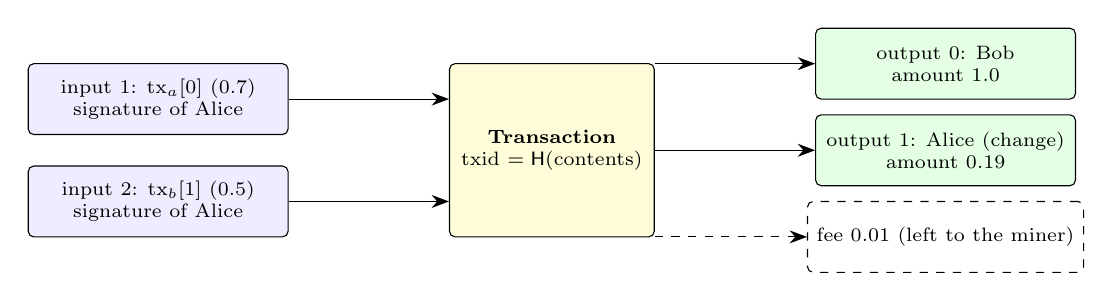
\begin{tikzpicture}[x=1cm,y=1cm,font=\scriptsize,
 bx/.style={draw,rounded corners=2pt,align=center,minimum height=0.9cm,minimum width=3.3cm}]
\node[bx,fill=blue!7] (i1) at (0,0.65) {input 1: tx$_a$[0] (0.7)\\ signature of Alice};
\node[bx,fill=blue!7] (i2) at (0,-0.65) {input 2: tx$_b$[1] (0.5)\\ signature of Alice};
\node[bx,fill=yellow!15,minimum height=2.2cm,minimum width=2.6cm] (t) at (5,0) {\textbf{Transaction}\\ txid $=\Hash(\text{contents})$};
\node[bx,fill=green!10] (o1) at (10,1.1) {output 0: Bob\\ amount 1.0};
\node[bx,fill=green!10] (o2) at (10,0) {output 1: Alice (change)\\ amount 0.19};
\node[bx,dashed] (f) at (10,-1.1) {fee 0.01 (left to the miner)};
\draw[->] (i1)--(t.west|-i1); \draw[->] (i2)--(t.west|-i2);
\draw[->] (t.east|-o1)--(o1); \draw[->] (t.east|-o2)--(o2); \draw[->,dashed] (t.east|-f)--(f);
\end{tikzpicture}
\caption{A transaction destroys two unspent outputs (total $1.2$) and creates two new ones; the difference is the fee.}
\end{figure}

\begin{oexbox}[paying with change]
Alice owns two unspent outputs, worth $0.7$ and $0.5$. She wants to pay Bob $1.0$. She cannot split a note, so she spends both ($1.2$ in total) and creates one output of $1.0$ for Bob and one output of $0.19$ back to herself (the \emph{change}). The remaining $1.2-1.0-0.19=0.01$ is the fee.
\end{oexbox}

\noindent A node accepts a transaction only if: (i) every input refers to an output that exists and is still unspent; (ii) no output is referenced twice; (iii) every signature is valid for the locking condition of the output it spends; (iv) the outputs add up to at most the inputs. Each full node maintains the set of all unspent outputs (the \emph{UTXO set}). A second transaction that tries to spend an output already spent violates (i) and is rejected; this is how double spending is prevented.

\subsection*{O.4\quad Merkle trees: summarising and verifying transactions}
A block may contain thousands of transactions, but the header has a fixed size. The \textbf{Merkle tree} bridges the gap. Its \emph{leaves} are the txids of the transactions. Every inner node is the hash of its two children concatenated, and the single hash at the top, the \textbf{Merkle root}, is stored in the header. (If a level has an odd number of nodes, the last one is duplicated.) Changing any transaction changes its leaf and therefore the root, so the header commits to the whole body.

\begin{figure}[htbp]
\centering
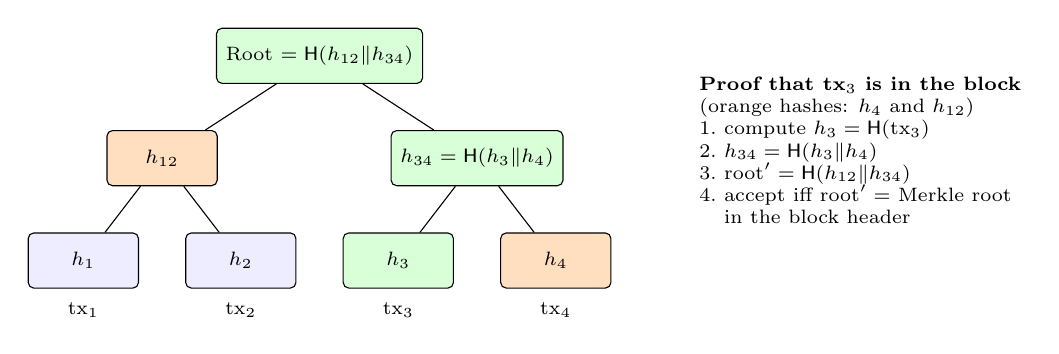
\begin{tikzpicture}[x=1cm,y=1cm,font=\scriptsize,
 n/.style={draw,rounded corners=2pt,minimum width=1.4cm,minimum height=0.7cm,align=center,fill=blue!7}]
\node[n,fill=green!15] (r) at (3,2.6) {Root $=\Hash(h_{12}\|h_{34})$};
\node[n,fill=orange!25] (a) at (1,1.3) {$h_{12}$};
\node[n,fill=green!15] (b) at (5,1.3) {$h_{34}=\Hash(h_3\|h_4)$};
\node[n] (l1) at (0,0) {$h_1$}; \node[n] (l2) at (2,0) {$h_2$};
\node[n,fill=green!15] (l3) at (4,0) {$h_3$}; \node[n,fill=orange!25] (l4) at (6,0) {$h_4$};
\foreach \l/\t in {l1/tx$_1$,l2/tx$_2$,l3/tx$_3$,l4/tx$_4$}{\node[below=0.05cm of \l] {\t};}
\draw (a)--(r); \draw (b)--(r); \draw (l1)--(a); \draw (l2)--(a); \draw (l3)--(b); \draw (l4)--(b);
\node[align=left,anchor=west] at (7.7,1.4) {\textbf{Proof that tx$_3$ is in the block}\\ (orange hashes: $h_4$ and $h_{12}$)\\ 1.\ compute $h_3=\Hash(\text{tx}_3)$\\ 2.\ $h_{34}=\Hash(h_3\|h_4)$\\ 3.\ $\text{root}'=\Hash(h_{12}\|h_{34})$\\ 4.\ accept iff $\text{root}'=$ Merkle root\\ \phantom{4.\ }in the block header};
\end{tikzpicture}
\caption{Merkle tree with four transactions and the proof of membership for tx$_3$.}
\end{figure}

To verify that a transaction is in a block, one does not need the block body. The prover supplies the \emph{sibling hash} at each level on the path from the transaction's leaf to the root (the \emph{Merkle path}); the verifier recomputes the path as in the figure above and compares the result with the Merkle root in the header. The proof has $\lceil\log_2n\rceil$ hashes for $n$ transactions. It is convincing because producing a different transaction with the same root would require a hash collision (Theorem~\ref{thm:merkle}).

\begin{oexbox}[size of a proof]
A block with $2000$ transactions of about $250$ bytes is roughly $500$ kB. A membership proof for one transaction consists of $\lceil\log_2 2000\rceil=11$ hashes of $32$ bytes, \ie\ $352$ bytes, and verification needs $12$ hash computations.
\end{oexbox}

\subsection*{O.5\quad Proof of work}
\textbf{The puzzle.} Anyone may propose the next block, so the network needs a fair, hard-to-fake way to choose the proposer. In Bitcoin a block is valid only if the hash of its header, read as a $256$-bit number, is smaller than the \emph{target} stored in the header:
$$\Hash(\Hash(\text{header}))<\text{target}.$$
A hash function behaves like a random function: there is no way to steer the output, so the miner changes the \emph{nonce} (and, when the nonce range is exhausted, other header fields) and recomputes the hash until a result falls below the target. Each attempt succeeds with probability $\text{target}/2^{256}$, independently of earlier attempts, so a miner with $10\%$ of the total computing power finds about $10\%$ of the blocks. A solution is easy to check (one hash) but costly to find.

\begin{figure}[htbp]
\centering
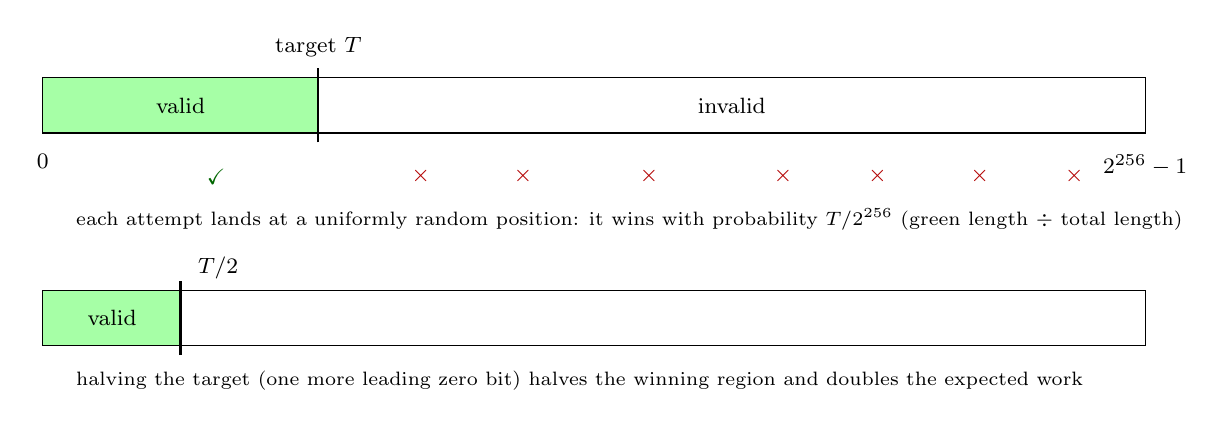
\begin{tikzpicture}[font=\footnotesize]
\def\W{14}
% bar for target T
\fill[green!35] (0,0) rectangle (3.5,0.7);
\draw (0,0) rectangle (\W,0.7);
\draw[thick] (3.5,-0.12)--(3.5,0.82);
\node[anchor=south] at (3.5,0.85) {target $T$};
\node at (1.75,0.35) {valid};
\node at (8.75,0.35) {invalid};
\node[below] at (0,-0.15) {$0$};
\node[below] at (\W,-0.15) {$2^{256}-1$};
\foreach \x in {6.1,9.4,11.9,4.8,13.1,7.7,10.6}{\node[red!70!black] at (\x,-0.55) {$\times$};}
\node[green!40!black] at (2.2,-0.55) {$\checkmark$};
\node[anchor=west,font=\scriptsize] at (0.3,-1.1) {each attempt lands at a uniformly random position: it wins with probability $T/2^{256}$ (green length $\div$ total length)};
% bar for T/2
\fill[green!35] (0,-2.7) rectangle (1.75,-2.0);
\draw (0,-2.7) rectangle (\W,-2.0);
\draw[thick] (1.75,-2.82)--(1.75,-1.88);
\node[anchor=south west] at (1.85,-1.98) {$T/2$};
\node at (0.88,-2.35) {valid};
\node[anchor=west,font=\scriptsize] at (0.3,-3.15) {halving the target (one more leading zero bit) halves the winning region and doubles the expected work};
\end{tikzpicture}
\caption{The target as a fraction of the hash space (not to scale: Bitcoin's real target is a fraction of order $2^{-76}$).}
\end{figure}

\textbf{What is the nonce?} The word is short for ``number used once''. It is a field of the header that carries no information at all: it is simply a number that the miner is free to choose. To see why it exists, note that once the miner has assembled a block, every other header field is fixed: the previous block hash, the Merkle root (determined by the chosen transactions), the timestamp and the target. The hash of a fixed header is one fixed number, so the miner would have exactly one attempt and nothing to vary if it failed. The nonce is the knob that the miner is allowed to turn. Changing the nonce by just $1$ changes the hash of the header completely and unpredictably, so every new nonce is a fresh, independent lottery ticket. The miner therefore does the following:
\begin{enumerate}[nosep,leftmargin=1.5em]
\item put $\text{nonce}=0$ in the header and compute $\Hash(\Hash(\text{header}))$;
\item if the result is below the target, stop: the block is valid;
\item otherwise add $1$ to the nonce and repeat from step~1.
\end{enumerate}
The winning nonce is the \emph{proof of work}. Nobody can predict a good nonce without trying, so showing one proves that, on average, a huge number of attempts were made. Checking it takes a single hash: insert the nonce into the header, hash once, and compare with the target. The nonce is not secret and need not be random (counting $0,1,2,\dots$ is fine; different miners just start at different values so they do not repeat each other's work).

\begin{figure}[htbp]
\centering
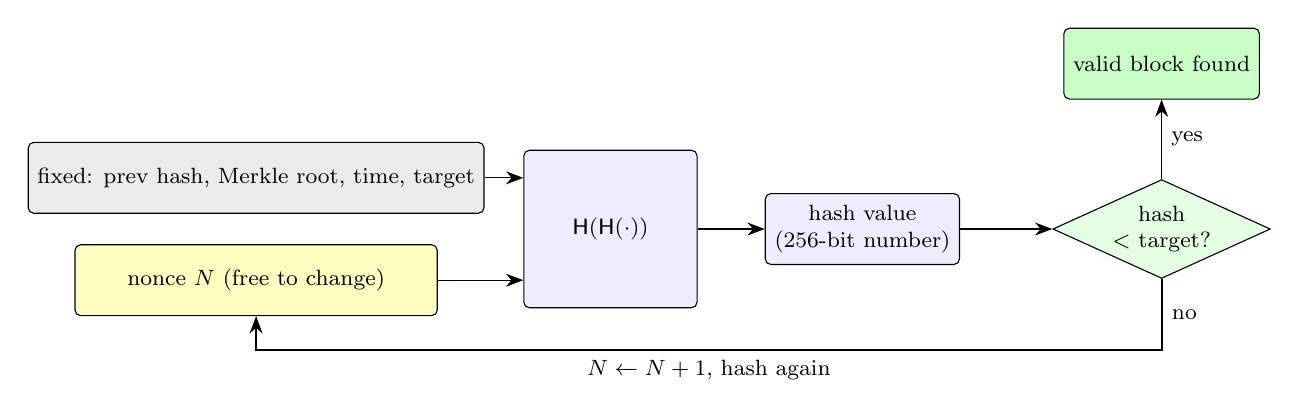
\begin{tikzpicture}[font=\footnotesize,
 bx/.style={draw,rounded corners=2pt,align=center,minimum height=0.9cm,fill=blue!7}]
\node[bx,fill=black!8,minimum width=4.6cm] (fix) at (0,0.65) {fixed: prev hash, Merkle root, time, target};
\node[bx,fill=yellow!25,minimum width=4.6cm] (non) at (0,-0.65) {nonce $N$ (free to change)};
\node[bx,minimum width=2.2cm,minimum height=2.0cm] (h) at (4.5,0) {$\Hash(\Hash(\cdot))$};
\node[bx,minimum width=2.4cm] (out) at (7.7,0) {hash value\\ ($256$-bit number)};
\node[draw,diamond,aspect=2.2,fill=green!10,inner sep=1pt,align=center] (dec) at (11.5,0) {hash\\ $<$ target?};
\node[bx,fill=green!22] (ok) at (11.5,2.1) {valid block found};
\draw[->] (fix.east)--(h.west|-fix); \draw[->] (non.east)--(h.west|-non);
\draw[->] (h)--(out); \draw[->] (out)--(dec);
\draw[->] (dec.north)--node[right]{yes}(ok.south);
\draw[->,thick] (dec.south)--++(0,-0.9) node[pos=0.5,right]{no} -| node[pos=0.25,below]{$N\leftarrow N+1$, hash again} (non.south);
\end{tikzpicture}
\caption{Mining is a loop: only the nonce changes between attempts.}
\end{figure}

In Bitcoin the nonce occupies $4$ bytes, \ie\ about $4.3$ billion values. Modern mining hardware tries them all in a fraction of a second, so miners also turn a second knob: they change a free field inside the coinbase transaction (the \emph{extra nonce}), which changes the Merkle root and thereby gives another $4.3$ billion fresh header hashes. The principle is the same: change something meaningless, get a new lottery ticket.

\begin{oexbox}[a toy puzzle]
Let the ``header'' be the text \texttt{prev=00ab12\allowbreak|merkle=9f3c47\allowbreak|time=1700000000\allowbreak|nonce=}$N$ and let the target be ``the SHA-256 hash starts with three hexadecimal zeros'' (probability $16^{-3}=1/4096$ per attempt).
\begin{center}\footnotesize
\begin{tabular}{@{}rl@{}}
\toprule
nonce $N$ & SHA-256 of the header (first 16 hex digits) \\
\midrule
0 & \texttt{42fff0e5f083da43\ldots} (fails)\\
1 & \texttt{cc1fc2610cd68dcf\ldots} (fails)\\
2 & \texttt{73939525c9d0d122\ldots} (fails)\\
\vdots & \vdots\\
2931 & \texttt{000b806c8c040726\ldots} (\textbf{success})\\
\bottomrule
\end{tabular}
\end{center}
Only the nonce changes between the rows, yet the hashes look completely unrelated. On average $4096$ attempts are needed; here $2932$ were (nonces $0$ to $2931$). Anybody can check the solution with one hash computation. Bitcoin's real target requires roughly $75$ to $80$ leading zero bits at recent network power (an order-of-magnitude figure), \ie\ about $2^{76}$ or more attempts per block.
\end{oexbox}

\textbf{Difficulty and the ten-minute rhythm.} If more miners join, blocks would come faster. Every $2016$ blocks the network compares the actual time $\tau$ with the intended $2016\cdot10$ minutes $=14$ days and rescales the target by $\tau/14$ days (at most a factor $4$ either way). If the last $2016$ blocks took $10$ days, the target shrinks by $10/14$, the puzzle becomes $1.4$ times harder, and the average interval returns to $10$ minutes.

\textbf{Why it provides security.} To change an old block, an attacker must redo its proof of work and that of every block after it, while the honest network keeps extending the chain. An attacker with less than half of the computing power succeeds with a probability that shrinks exponentially in the number of blocks on top of the transaction (its \emph{confirmations}); about $6$ confirmations are customary (Part~4 derives this).

\textbf{Why miners take part.} The coinbase transaction pays the miner the block reward (initially $50$ coins, halved every $210{,}000$ blocks, about every four years; it has been $3.125$ coins since April 2024) plus the fees of all included transactions. Miners spend real electricity on the puzzle, so honest mining is the best way to earn this income.

\subsection*{O.6\quad Putting it together: adding a block}
\begin{figure}[htbp]
\centering
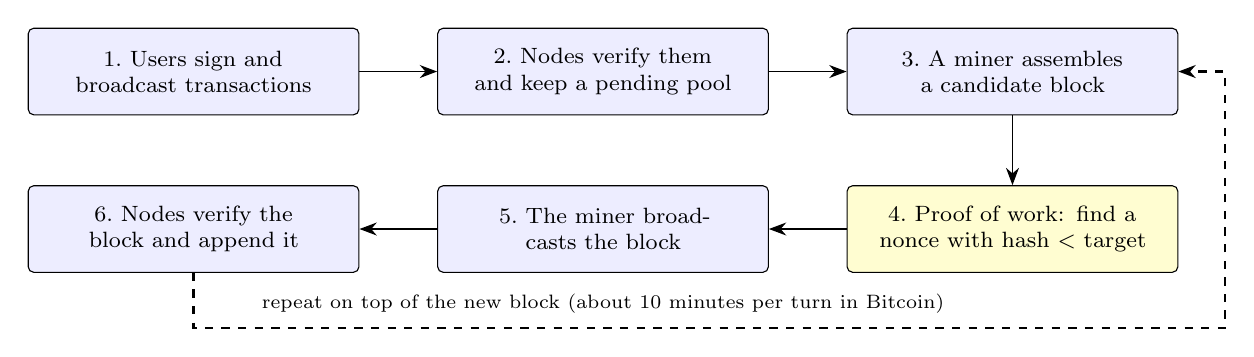
\begin{tikzpicture}[font=\footnotesize,
 st/.style={draw,rounded corners=2pt,minimum width=4.2cm,text width=3.9cm,minimum height=1.1cm,align=center,fill=blue!7}]
\node[st] (a) at (0,0) {1.\ Users sign and broadcast transactions};
\node[st] (b) at (5.2,0) {2.\ Nodes verify them and keep a pending pool};
\node[st] (c) at (10.4,0) {3.\ A miner assembles a candidate block};
\node[st,fill=yellow!18] (d) at (10.4,-2) {4.\ Proof of work: find a nonce with hash $<$ target};
\node[st] (e) at (5.2,-2) {5.\ The miner broadcasts the block};
\node[st] (f) at (0,-2) {6.\ Nodes verify the block and append it};
\draw[->] (a)--(b); \draw[->] (b)--(c); \draw[->] (c)--(d); \draw[->] (d)--(e); \draw[->] (e)--(f);
\draw[->,thick,dashed] (f.south) -- ++(0,-0.7) -| (13.1,0) -- (c.east);
\node[font=\scriptsize] at (5.2,-2.95) {repeat on top of the new block (about $10$ minutes per turn in Bitcoin)};
\end{tikzpicture}
\caption{The block production cycle.}
\end{figure}
Anyone can create a transaction, sign it, and broadcast it. Every node that receives it checks the four rules of Section~O.3 and keeps it in its pool of pending transactions. On average every $10$ minutes some miner finds a valid nonce for a block of pending transactions (usually the best-paying ones, with the coinbase first) built on the current chain tip, and broadcasts it. Every node verifies the proof of work and every transaction in the block. If all checks pass, it appends the block to its copy of the chain, deletes the included transactions from its pending pool, and starts mining on top of the new block. If two blocks are found at nearly the same time, nodes keep both for a while and follow the chain with the most accumulated work; the other branch is abandoned and its transactions return to the pending pool. Section~O.8 shows who tells whom and what happens when some nodes misbehave.

\subsection*{O.7\quad Full nodes and light nodes}
Not everybody can store and verify the whole chain, which is hundreds of gigabytes. Two kinds of participants therefore exist.

\begin{center}
\footnotesize\renewcommand{\arraystretch}{0.95}
\begin{tabular}{@{}p{2.2cm}p{6.6cm}p{6.6cm}@{}}
\toprule
 & \textbf{Full node} & \textbf{Light node (SPV client, phone wallet)}\\
\midrule
Stores & all blocks, all transactions, the UTXO set & only the block headers ($80$ bytes each, under $100$ MB in total)\\
Verifies & every rule: proof of work, signatures, no double spend & proof of work of each header; Merkle proofs for its own transactions\\
Trusts & nobody for validity & that the most-work chain contains only valid blocks (an honest-majority assumption) and that its peers pass on information\\
Role & relays transactions and blocks, serves data to others & asks full nodes for data\\
\bottomrule
\end{tabular}
\end{center}

A light node cannot find out by itself which transactions concern it or whether they were included, because it holds no transactions. It therefore asks full nodes. It needs them to
\begin{enumerate}[nosep,leftmargin=1.5em]
\item send the block headers, from which it builds and checks the header chain (each header must satisfy its proof of work and point to the previous one);
\item return the transactions that involve its addresses, each with the block it belongs to and its Merkle path;
\item accept and relay the transactions it wants to broadcast.
\end{enumerate}

\begin{figure}[htbp]
\centering
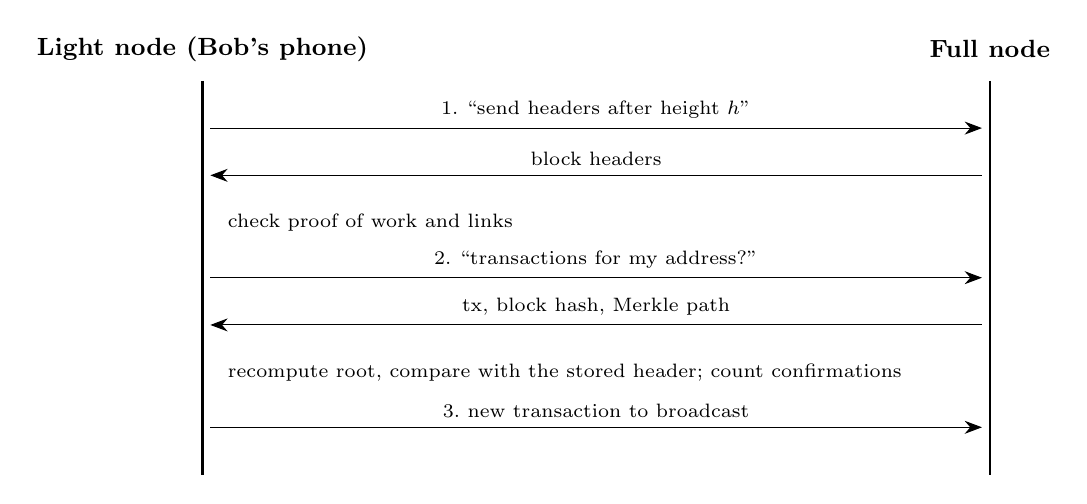
\begin{tikzpicture}[x=1cm,y=1cm,font=\scriptsize]
\node[font=\small\bfseries] at (0,0) {Light node (Bob's phone)};
\node[font=\small\bfseries] at (10,0) {Full node};
\draw[thick] (0,-0.4)--(0,-5.4); \draw[thick] (10,-0.4)--(10,-5.4);
\draw[->] (0.1,-1)--node[above]{1.\ ``send headers after height $h$''}(9.9,-1);
\draw[<-] (0.1,-1.6)--node[above]{block headers}(9.9,-1.6);
\node[anchor=west] at (0.2,-2.2) {check proof of work and links};
\draw[->] (0.1,-2.9)--node[above]{2.\ ``transactions for my address?''}(9.9,-2.9);
\draw[<-] (0.1,-3.5)--node[above]{tx, block hash, Merkle path}(9.9,-3.5);
\node[anchor=west] at (0.2,-4.1) {recompute root, compare with the stored header; count confirmations};
\draw[->] (0.1,-4.8)--node[above]{3.\ new transaction to broadcast}(9.9,-4.8);
\end{tikzpicture}
\caption{What a light node asks of a full node.}
\end{figure}

\begin{oexbox}[Bob checks a payment on his phone]
Alice says she paid Bob. Bob's phone already has all headers. It asks a full node for transactions to Bob's address and receives tx$_3$ together with the hash of the block $B_{k}$ and a Merkle path of $11$ hashes. The phone recomputes the root from tx$_3$ and the path, compares it with the Merkle root in its stored header of $B_k$, and counts the headers above $B_k$: if there are $6$, the payment has $6$ confirmations. The phone downloaded a few hundred bytes instead of the block.
\end{oexbox}

\noindent\textbf{Limits of light nodes.} Because it checks only inclusion and proof of work, a light node cannot detect an invalid transaction hidden inside a block of the heaviest chain; it relies on the honest-majority assumption. A dishonest full node can hide a transaction by simply not reporting it, so light nodes connect to several full nodes. The requests also reveal which addresses the user cares about, a privacy cost. Full nodes are therefore the backbone that enforces the rules, and light nodes are an efficient but less trustless way to use the network.


\subsection*{O.8\quad The peer-to-peer network: communication, bad miners and trust}
So far we described blocks and transactions. This section explains how the computers actually talk to each other, what happens when some of them misbehave or refuse to cooperate, and why nobody has to be trusted.

\textbf{Who is in the network.} There is no central server. Every participant, called a \emph{node}, runs the same open-source software and keeps connections to a few \emph{peers}: in Bitcoin about $8$ outgoing connections to randomly chosen nodes plus incoming ones. A newcomer finds its first peers through a few well-known seed servers and then learns more addresses by asking its peers. Figure~\ref{fig:p2p} draws every participant as a circle.
\begin{itemize}[nosep,leftmargin=1.2em]
\item \textbf{Full miner} (yellow): a full node that also searches for blocks. A \emph{mining pool} operator (like $M_2$) is a full miner that hands work to many small machines.
\item \textbf{Full node} (blue): stores the whole chain and checks every rule, but does not mine. It is the referee of the system and the main relay between the others.
\item \textbf{Light node} (dashed): a phone wallet that keeps only headers (Section~O.7). It asks full nodes for data and does not forward blocks.
\item \textbf{Pool (light) miner} (dotted): mining hardware that stores no chain. The pool operator sends it a ready-made header to work on (the operator chooses the transactions), and it returns nonces that solve the puzzle, or an easier version of it that proves it is working. It lends hash power but relies on the operator for the contents of the block.
\end{itemize}
One person may play several roles; what matters is what each machine checks.

\textbf{How news travels: gossip.} Nodes only talk to their direct peers; nobody broadcasts to everybody. News spreads like a rumour: when a node learns something new it first \emph{verifies} it and only then tells its peers, who verify it and tell theirs. To avoid sending large objects again and again, a node first announces only a short hash (\texttt{inv}); a peer that does not have the object replies \texttt{getdata}, and only then the transaction or block itself is sent (Figure~\ref{fig:relay}). Since every node has several peers and there are many paths, a new block reaches almost everybody within seconds (Figure~\ref{fig:waves}), and a few silent or lying nodes cannot stop the flow.

\begin{figure}[htbp]
\centering
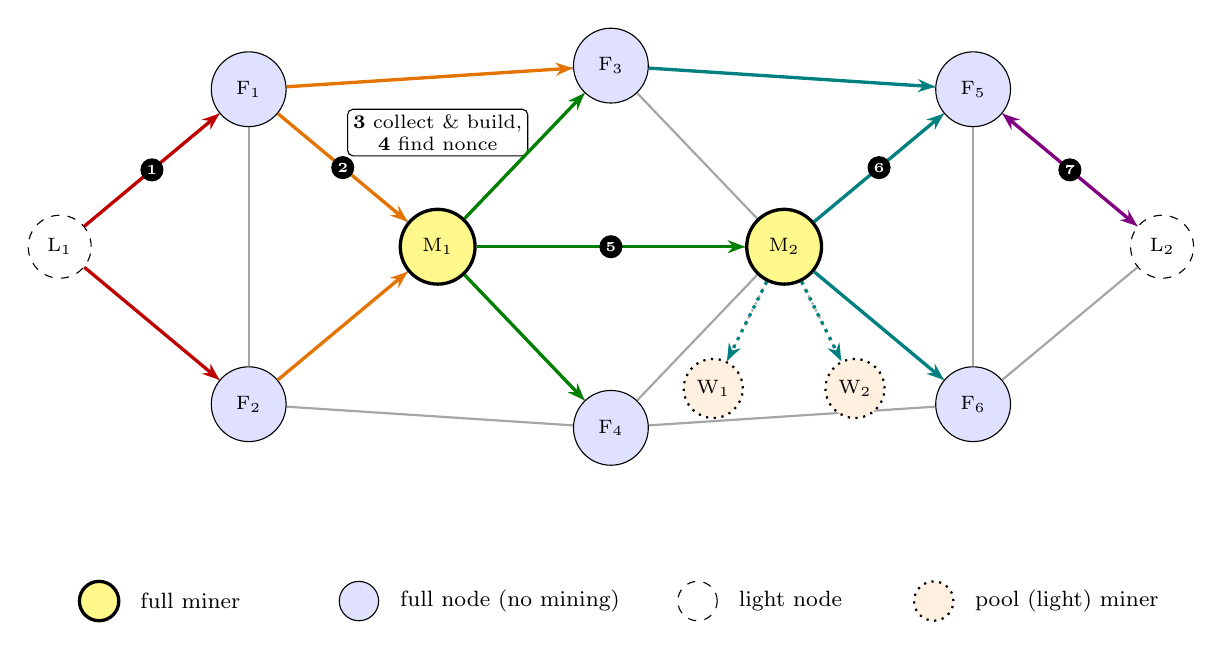
\begin{tikzpicture}[font=\footnotesize]
\foreach \n/\x/\y/\l/\st in {L1/0/3/L$_1$/nL, F1/2.4/5/F$_1$/nF, F2/2.4/1/F$_2$/nF, M1/4.8/3/M$_1$/nM, F3/7/5.3/F$_3$/nF, F4/7/0.7/F$_4$/nF, M2/9.2/3/M$_2$/nM, F5/11.6/5/F$_5$/nF, F6/11.6/1/F$_6$/nF, L2/14/3/L$_2$/nL, W1/8.3/1.2/W$_1$/nW, W2/10.1/1.2/W$_2$/nW}{\node[\st] (\n) at (\x,\y) {\l};}
\begin{scope}[on background layer]
\foreach \a/\b in {L1/F1,L1/F2,F1/F2,F1/M1,F2/M1,F1/F3,F2/F4,M1/F3,M1/F4,M1/M2,F3/M2,F4/M2,F3/F5,F4/F6,M2/F5,M2/F6,F5/F6,F5/L2,F6/L2}{\draw[gray!70,thick] (\a)--(\b);}
\foreach \a/\b in {M2/W1,M2/W2}{\draw[gray!70,thick,dotted] (\a)--(\b);}
\end{scope}
\draw[->,very thick,red!75!black] (L1)--(F1) node[midway,badge]{1};
\draw[->,very thick,red!75!black] (L1)--(F2);
\draw[->,very thick,orange!90!black] (F1)--(M1) node[midway,badge]{2};
\draw[->,very thick,orange!90!black] (F2)--(M1);
\draw[->,very thick,orange!90!black] (F1)--(F3);
\node[draw,rounded corners=2pt,fill=white,font=\scriptsize,align=center,inner sep=2pt] at (4.8,4.45) {\textbf{3} collect \& build,\\ \textbf{4} find nonce};
\draw[->,very thick,green!50!black] (M1)--(M2) node[midway,badge]{5};
\draw[->,very thick,green!50!black] (M1)--(F3);
\draw[->,very thick,green!50!black] (M1)--(F4);
\draw[->,very thick,teal] (M2)--(F5) node[midway,badge]{6};
\draw[->,very thick,teal] (M2)--(F6);
\draw[->,very thick,teal] (F3)--(F5);
\draw[->,very thick,teal,dotted] (M2)--(W1);
\draw[->,very thick,teal,dotted] (M2)--(W2);
\draw[<->,very thick,violet] (L2)--(F5) node[midway,badge]{7};
\begin{scope}[yshift=-1.5cm,xshift=0.5cm]\netlegend\end{scope}
\end{tikzpicture}
\caption{A small network and the life of Alice's payment to Bob. Grey lines are peer connections. Each circle is a computer. The numbers are the steps explained in the text: (1) submit, (2) check and relay, (3)--(4) collect transactions and find a block, (5) announce the block, (6) verify, update and forward (the pool operator $M_2$ also sends fresh work to its workers), (7) light node $L_2$ fetches headers and a Merkle proof.}
\label{fig:p2p}
\end{figure}

\textbf{A payment travelling through the network} (Figure~\ref{fig:p2p}). Alice's phone $L_1$ pays Bob, whose phone is $L_2$.
\begin{enumerate}[nosep,leftmargin=1.5em]
\item \emph{Submit.} $L_1$ signs the transaction and sends it to the full nodes it is connected to ($F_1$, $F_2$). A light node cannot check the transaction itself, since it has no UTXO set.
\item \emph{Check and relay.} $F_1$ checks the four rules of Section~O.3 against its UTXO set. If they hold, it stores the transaction in its pending pool and announces it to its peers; if not, it drops it silently, so invalid transactions die at the first honest node. Within seconds most nodes, including the miners, hold the transaction.
\item \emph{Collect.} Miner $M_1$ takes pending transactions, preferring high fees, adds its coinbase transaction and builds a candidate block (Section~O.6).
\item \emph{Find.} $M_1$ (or a worker $W_i$ of a pool, which reports its winning nonce to the operator) finds a nonce with hash below the target.
\item \emph{Announce the block.} $M_1$ announces the block to its peers ($F_3$, $F_4$, $M_2$). Peers usually already hold most of its transactions, so a \emph{compact block} with short transaction identifiers is enough.
\item \emph{Verify, update, forward.} Each receiving node verifies the proof of work, the link to its current tip and every transaction \emph{before} relaying (validate, then forward). It then appends the block, updates its UTXO set, deletes the included transactions from its pending pool and starts mining on the new tip. A pool operator sends fresh work to its workers, because work on the old tip is wasted.
\item \emph{Inform the light nodes.} $L_2$ asks a full node for new headers and for the Merkle path of Alice's transaction (Section~O.7), checks them and counts confirmations as further blocks arrive.
\end{enumerate}

\begin{figure}[htbp]
\centering
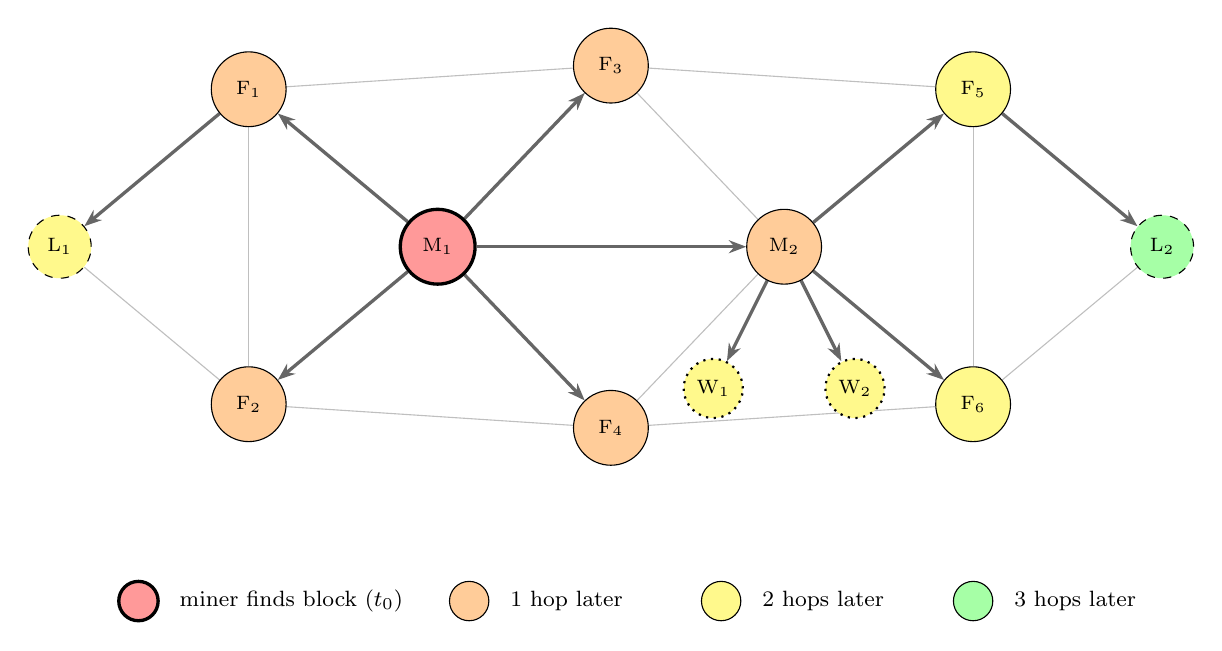
\begin{tikzpicture}[font=\footnotesize]
\foreach \n/\x/\y/\l/\st in {L1/0/3/L$_1$/h2d, F1/2.4/5/F$_1$/h1, F2/2.4/1/F$_2$/h1, M1/4.8/3/M$_1$/h0, F3/7/5.3/F$_3$/h1, F4/7/0.7/F$_4$/h1, M2/9.2/3/M$_2$/h1, F5/11.6/5/F$_5$/h2, F6/11.6/1/F$_6$/h2, L2/14/3/L$_2$/h3d, W1/8.3/1.2/W$_1$/h2t, W2/10.1/1.2/W$_2$/h2t}{\node[\st] (\n) at (\x,\y) {\l};}
\begin{scope}[on background layer]
\foreach \a/\b in {L1/F2,F1/F2,F2/F4,F1/F3,M1/F3,F3/M2,F4/M2,F3/F5,F4/F6,F5/F6,F6/L2}{\draw[gray!50] (\a)--(\b);}
\foreach \a/\b in {M1/F1,M1/F2,M1/F3,M1/F4,M1/M2,F1/L1,M2/F5,M2/F6,M2/W1,M2/W2,F5/L2}{\draw[->,very thick,gray!80!black] (\a)--(\b);}
\end{scope}
\begin{scope}[yshift=-1.5cm,xshift=1cm]
\node[h0,minimum size=0.5cm] at (0,0) {}; \node[anchor=west] at (0.4,0) {miner finds block ($t_0$)};
\node[h1,minimum size=0.5cm] at (4.2,0) {}; \node[anchor=west] at (4.6,0) {1 hop later};
\node[h2,minimum size=0.5cm] at (7.4,0) {}; \node[anchor=west] at (7.8,0) {2 hops later};
\node[h3,minimum size=0.5cm] at (10.6,0) {}; \node[anchor=west] at (11.0,0) {3 hops later};
\end{scope}
\end{tikzpicture}
\caption{How a new block spreads. Thick arrows show along which connection each node heard of the block first; colours show the number of hops from the miner. The network is covered within a few hops, each taking a fraction of a second to a second. Light nodes (dashed) learn about it when they next ask a full node for headers.}
\label{fig:waves}
\end{figure}

\begin{figure}[htbp]
\centering
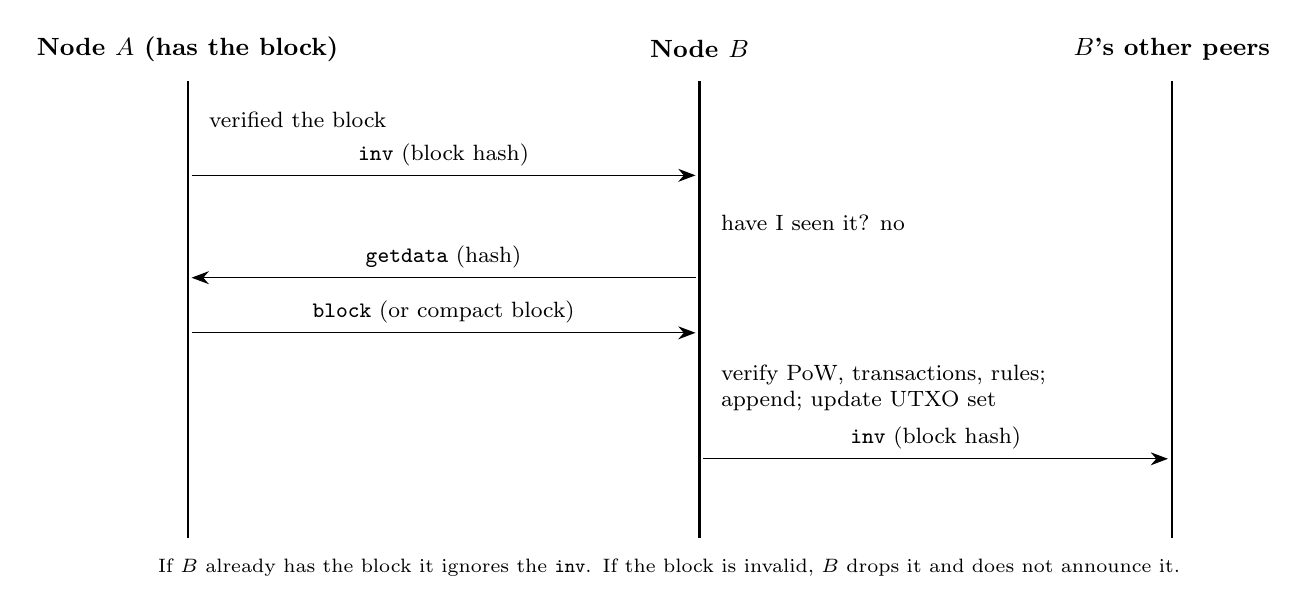
\begin{tikzpicture}[font=\footnotesize]
\node[font=\small\bfseries] at (0,0) {Node $A$ (has the block)};
\node[font=\small\bfseries] at (6.5,0) {Node $B$};
\node[font=\small\bfseries] at (12.5,0) {$B$'s other peers};
\foreach \x in {0,6.5,12.5}{\draw[thick] (\x,-0.4)--(\x,-6.2);}
\node[anchor=west,align=left] at (0.15,-0.9) {verified the block};
\draw[->] (0.05,-1.6)--node[above]{\texttt{inv} (block hash)}(6.45,-1.6);
\node[anchor=west,align=left] at (6.65,-2.2) {have I seen it? no};
\draw[<-] (0.05,-2.9)--node[above]{\texttt{getdata} (hash)}(6.45,-2.9);
\draw[->] (0.05,-3.6)--node[above]{\texttt{block} (or compact block)}(6.45,-3.6);
\node[anchor=west,align=left] at (6.65,-4.3) {verify PoW, transactions, rules;\\ append; update UTXO set};
\draw[->] (6.55,-5.2)--node[above]{\texttt{inv} (block hash)}(12.45,-5.2);
\node[anchor=north west,align=left,font=\scriptsize,text width=13cm] at (-0.5,-6.35) {If $B$ already has the block it ignores the \texttt{inv}. If the block is invalid, $B$ drops it and does not announce it.};
\end{tikzpicture}
\caption{The announce--request pattern between two neighbours. Only the short hash is sent unasked; the full block is sent once, on request, and is forwarded only after it has been verified.}
\label{fig:relay}
\end{figure}

\textbf{Catching up and bootstrapping.} A node that was offline, or is new, connects to peers and asks for their headers (\texttt{getheaders}). It checks each proof of work, picks the header chain with the most work, downloads the blocks and verifies all of them from the first block, the \emph{genesis block}, whose hash is fixed in the software. Besides the software itself, this is the only thing it takes on trust. From then on it follows the gossip described above.

\textbf{What if some miners misbehave or do not cooperate?} Figure~\ref{fig:rogue} shows a rogue miner $R$ (red) among honest nodes. The table lists typical misbehaviours.

\begin{center}
\footnotesize\renewcommand{\arraystretch}{1.05}
\begin{tabular}{@{}p{3.6cm}p{5.6cm}p{6.0cm}@{}}
\toprule
\textbf{Behaviour} & \textbf{What honest nodes do} & \textbf{Why the damage is limited}\\
\midrule
Broadcasts an \emph{invalid} block (forged signature, spends a non-existent coin, pays itself too much, hash not below target) & Every honest full node rejects it at the first hop and does not forward it & The miner wasted its electricity; peers may disconnect it\\\addlinespace[4pt]
Stays silent, relays nothing, or ignores some transactions & Transactions and blocks reach others over other peers; non-mining full nodes relay as well & A transaction waits until an honest miner finds a block: about $1/(1-q)$ blocks on average, \eg\ $1.4$ for a miner with $q=30\%$\\\addlinespace[4pt]
Finds valid blocks but keeps them secret (selfish mining, double spending) & Does not know about them and continues; if the secret chain is published later and has less work, it is ignored & Pays only with a large share of the hash power (Part~4)\\\addlinespace[4pt]
Mines its own \emph{valid} but different chain, ignoring the others' blocks & Stores it as a side branch but keeps following the chain with the most work & Its rewards lie on a branch nobody extends, so they are worthless; following the main chain is the rational choice\\\addlinespace[4pt]
Changes the rules (larger blocks, larger reward) & Its blocks are invalid under the rules honest nodes run, so they are rejected & If a group of users adopts the new rules too, the system splits permanently into two networks and two currencies (a \emph{hard fork}, \eg\ Bitcoin and Bitcoin Cash in 2017); otherwise the rule-changer is ignored\\\addlinespace[4pt]
Surrounds a victim with its own nodes (\emph{eclipse}) or floods the network with fake nodes (\emph{Sybil}) & Nodes choose peers at random and keep many connections; a victim needs only \emph{one} honest peer to learn the heaviest valid chain & Light nodes are more exposed than full nodes, so they connect to several full nodes\\\addlinespace[4pt]
Controls more than $50\%$ of the hash power & Can rewrite recent history and censor transactions & Still cannot forge signatures, spend other people's coins or break the rules (Part~4)\\
\bottomrule
\end{tabular}
\end{center}

\begin{figure}[htbp]
\centering
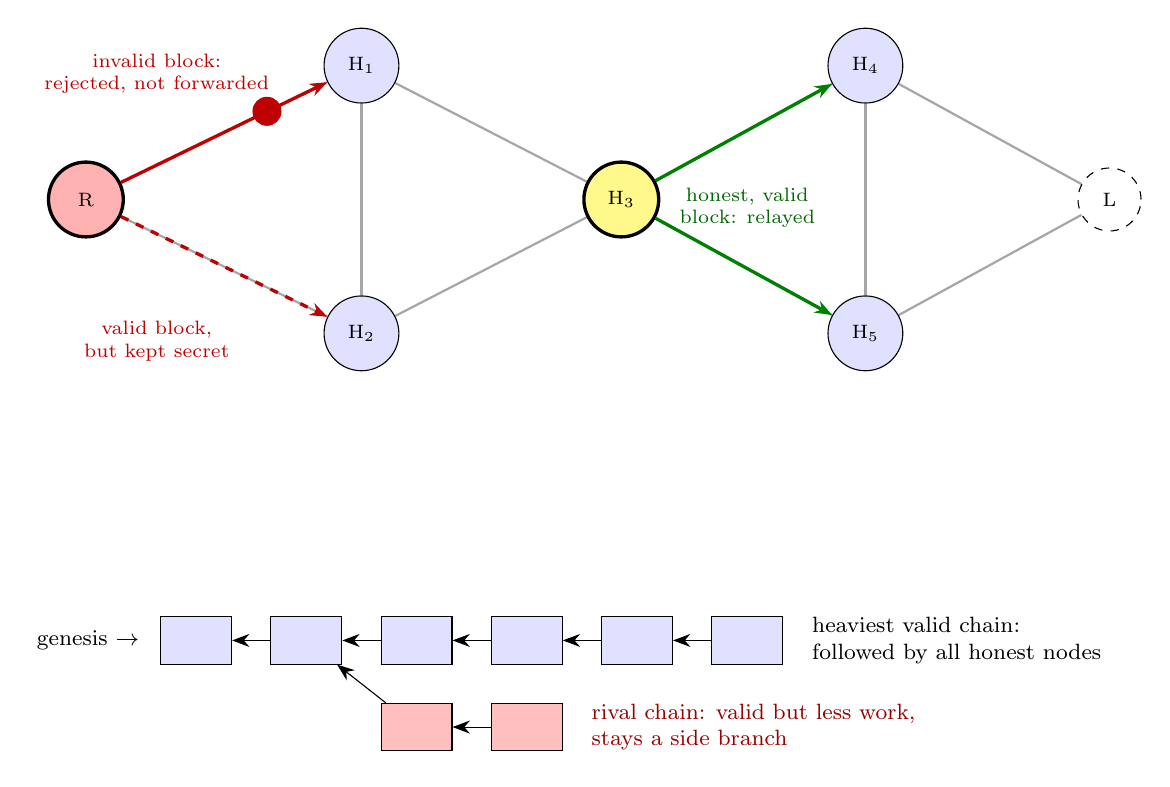
\begin{tikzpicture}[font=\footnotesize]
\foreach \n/\x/\y/\l/\st in {R/0.8/2/R/nB, H1/4.3/3.7/H$_1$/nF, H2/4.3/0.3/H$_2$/nF, H3/7.6/2/H$_3$/nM, H4/10.7/3.7/H$_4$/nF, H5/10.7/0.3/H$_5$/nF, H6/13.8/2/L/nL}{\node[\st] (\n) at (\x,\y) {\l};}
\begin{scope}[on background layer]
\foreach \a/\b in {R/H1,R/H2,H1/H2,H1/H3,H2/H3,H3/H4,H3/H5,H4/H5,H4/H6,H5/H6}{\draw[gray!70,thick] (\a)--(\b);}
\end{scope}
\draw[->,very thick,red!75!black] (R)--(H1);
\node[circle,fill=white,draw=red!75!black,inner sep=0.5pt,font=\bfseries\footnotesize,red!75!black] at (3.1,3.12) {$\times$};
\node[red!75!black,font=\scriptsize,align=center] at (1.7,3.6) {invalid block:\\ rejected, not forwarded};
\draw[->,very thick,red!75!black,dashed] (R)--(H2);
\node[red!75!black,font=\scriptsize,align=center] at (1.7,0.2) {valid block,\\ but kept secret};
\draw[->,very thick,green!50!black] (H3)--(H4);
\draw[->,very thick,green!50!black] (H3)--(H5);
\node[green!40!black,font=\scriptsize,align=center] at (9.2,1.9) {honest, valid\\ block: relayed};
\begin{scope}[yshift=-3.6cm]
\foreach \i in {0,...,5}{\node[draw,minimum width=0.9cm,minimum height=0.6cm,fill=blue!12] (c\i) at ({2.2+1.4*\i},0) {};}
\foreach \i/\j in {1/0,2/1,3/2,4/3,5/4}{\draw[->] (c\i)--(c\j);}
\node[draw,minimum width=0.9cm,minimum height=0.6cm,fill=red!25] (r2) at ({2.2+1.4*2},-1.1) {};
\node[draw,minimum width=0.9cm,minimum height=0.6cm,fill=red!25] (r3) at ({2.2+1.4*3},-1.1) {};
\draw[->] (r2)--(c1); \draw[->] (r3)--(r2);
\node[anchor=east] at (1.6,0) {genesis $\to$};
\node[anchor=west,align=left] at (9.9,0) {heaviest valid chain:\\ followed by all honest nodes};
\node[anchor=west,align=left,red!60!black] at (7.1,-1.1) {rival chain: valid but less work,\\ stays a side branch};
\end{scope}
\end{tikzpicture}
\caption{A rogue miner $R$ among honest nodes. Top: what the network does with what $R$ sends. An invalid block is dropped at the first honest node; a secretly mined valid chain is unknown to others. Bottom: even if the rival chain is shown later, honest nodes keep following the chain with the most work.}
\label{fig:rogue}
\end{figure}

\textbf{What does ``the blockchain'' mean when copies differ?} There is no master copy. Every node holds its own local copy. Copies differ briefly near the tip (a new block has not reached everybody, or two blocks were found at once) but agree on everything older; this is the \emph{common prefix} property proved in Part~4. So ``the blockchain'' is the \emph{valid chain with the most accumulated work that the honest nodes follow}. A rogue miner's private chain is not a second blockchain of the system: if it breaks the rules it is simply invalid, and if it obeys the rules but has less work it is an orphaned side branch. Only when a sizeable group of users deliberately changes the rules does a second, independent system appear, and each user chooses which one to join by the software they run. In short: miners decide which valid block comes next, but full nodes decide what ``valid'' means.

\textbf{Whom do we trust?} Nobody in particular. A full node does not ask who sent a block; it applies the procedure of Figure~\ref{fig:decide} to every block from every peer. It takes on trust only (i) the software and the genesis block hash, and (ii) the assumption that most of the hash power is honest, which is what makes the most-work chain a reliable record. A light node additionally trusts that the most-work chain contains no invalid blocks and that at least one of its peers is honest.

\begin{figure}[htbp]
\centering
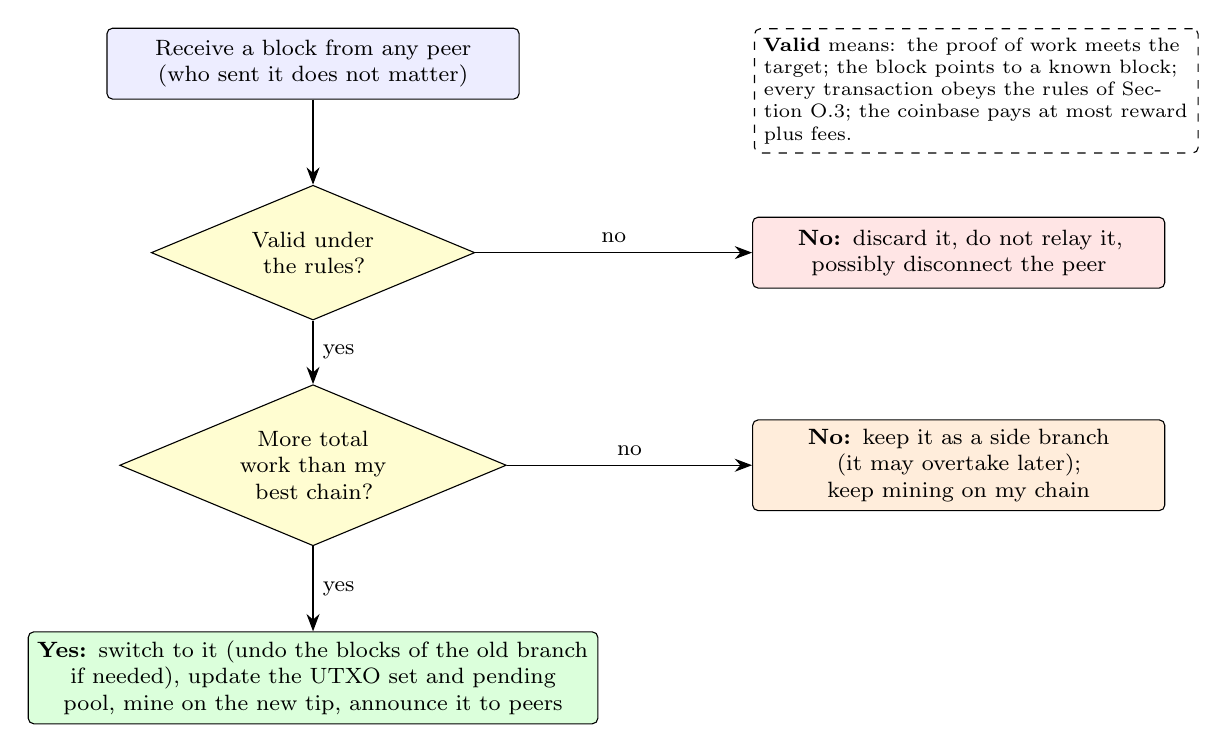
\begin{tikzpicture}[font=\footnotesize,
 bx/.style={draw,rounded corners=2pt,align=center,fill=blue!7,text width=5.0cm,minimum height=0.9cm},
 dc/.style={draw,diamond,aspect=2.4,align=center,fill=yellow!18,inner sep=1pt,text width=2.6cm}]
\node[bx] (r) at (0,0) {Receive a block from any peer\\ (who sent it does not matter)};
\node[dc] (v) at (0,-2.4) {Valid under the rules?};
\node[bx,fill=red!10] (x) at (8.2,-2.4) {\textbf{No:} discard it, do not relay it, possibly disconnect the peer};
\node[dc] (w) at (0,-5.1) {More total work than my best chain?};
\node[bx,fill=orange!14] (s) at (8.2,-5.1) {\textbf{No:} keep it as a side branch (it may overtake later); keep mining on my chain};
\node[bx,fill=green!14,text width=7cm] (a) at (0,-7.8) {\textbf{Yes:} switch to it (undo the blocks of the old branch if needed), update the UTXO set and pending pool, mine on the new tip, announce it to peers};
\draw[->] (r)--(v); \draw[->] (v)--node[right]{yes}(w); \draw[->] (w)--node[right]{yes}(a);
\draw[->] (v)--node[above]{no}(x); \draw[->] (w)--node[above]{no}(s);
\node[draw,dashed,rounded corners=2pt,align=left,font=\scriptsize,text width=5.4cm,anchor=north west] at (5.6,0.45) {\textbf{Valid} means: the proof of work meets the target; the block points to a known block; every transaction obeys the rules of Section~O.3; the coinbase pays at most reward plus fees.};
\end{tikzpicture}
\caption{The decision procedure of a full node for every block it hears of. It uses only public rules and the accumulated work; no peer and no miner has to be trusted.}
\label{fig:decide}
\end{figure}

\normalsize
\newpage

\section*{How to read these notes}
Every topic follows the same rhythm: first the idea is explained in ordinary language, with no formulas; then the formal definitions, theorems and proofs are given; finally worked examples with concrete numbers (marked \emph{Example}, ending with $\triangleleft$) show the mathematics in action. Warnings mark common misconceptions and attacks. Each part ends with exercises; hints and answers to the numerical ones are collected in the appendix. For a gentle textbook introduction to the same material see~\cite{BMC15}.

\paragraph{Suggested timing (about 3.5 hours with questions).}
\begin{center}
\begin{tabular}{@{}clr@{}}
\toprule
Part & Topic & Minutes\\
\midrule
1 & Motivation, problem statement, threat model & 10\\
2 & Cryptographic building blocks & 25\\
3 & Bitcoin in detail & 35\\
4 & Security analysis of Nakamoto consensus & 35\\
5 & Consensus theory (BFT, PBFT, Proof-of-Stake) & 30\\
6 & Smart contracts and Ethereum & 15\\
7 & Privacy-preserving blockchains & 30\\
8 & Advanced topics (BLS, threshold, VDF, MEV, quantum) & 20\\
9 & Open problems and wrap-up & 10\\
\midrule
 & Total & 210\\
\bottomrule
\end{tabular}
\end{center}

\paragraph{Notation.} $\lambda$ (or $\kappa$) is the security parameter. $\Hash$ is a hash function with
$n$-bit output. $\negl(\lambda)$ is a negligible function. $x\leftarrow_{\$}S$ means $x$ is sampled
uniformly from $S$. $\|$ is concatenation.

%================================================================
\section{Motivation, Problem Statement and Threat Model}\label{sec:motivation}
%================================================================

\subsection{Why do we need a blockchain at all?}

\begin{plainenglish}
Suppose Alice wants to pay Bob over the Internet. Digital information can be copied for free, so
what stops Alice from sending the \emph{same} digital coin to Bob and to Carol? This is the
\textbf{double-spending problem}. For physical cash it does not exist (a banknote can only be in one
pocket). For digital money the traditional fix is a \textbf{trusted third party}: a bank keeps a
ledger (a list of who owns what) and refuses a second spend of the same money.

A blockchain answers a different question: \emph{can a group of mutually distrusting computers, with
no boss, agree on a single ledger, even if some of them are cheating?} Bitcoin~\cite{Nak08} was the first practical answer.
\end{plainenglish}

\begin{figure}[htbp]
\centering
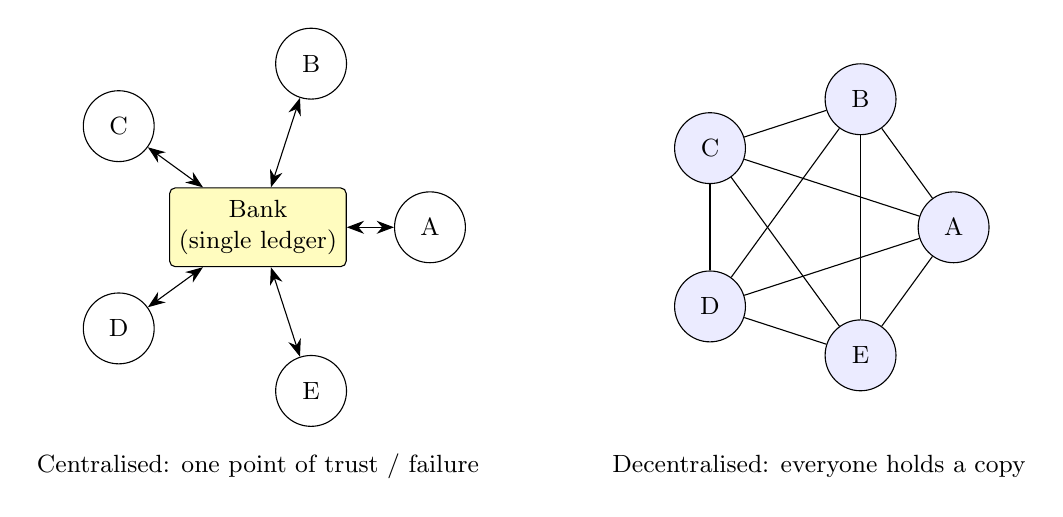
\begin{tikzpicture}[scale=0.95]
% left: centralised
\node[blk,fill=yellow!25] (bank) at (0,0) {Bank\\(single ledger)};
\foreach \a/\n in {0/A,72/B,144/C,216/D,288/E}{
  \node[node] (c\n) at (\a:2.3) {\n};
  \draw[<->] (bank) -- (c\n);
}
\node at (0,-3.2) {\small Centralised: one point of trust / failure};
% right: decentralised
\begin{scope}[xshift=7.5cm]
\foreach \a/\n in {0/A,72/B,144/C,216/D,288/E}{
  \node[node,fill=blue!8] (d\n) at (\a:1.8) {\n};
}
\foreach \x/\y in {A/B,B/C,C/D,D/E,E/A,A/C,B/D,C/E,D/A,E/B}{ \draw (d\x)--(d\y); }
\node at (0,-3.2) {\small Decentralised: everyone holds a copy};
\end{scope}
\end{tikzpicture}
\caption{Centralised ledger versus replicated ledger.}
\end{figure}

\begin{exbox}[double spending]
Alice owns 1 coin, represented by the string \texttt{coin\#4711}. She sends a message
``\texttt{pay coin\#4711 to Bob}'' to Bob and, at the same moment, ``\texttt{pay coin\#4711 to Carol}''
to Carol. Both messages carry valid signatures from Alice. Bob and Carol cannot tell by looking at
their own messages that anything is wrong. Only a \emph{global agreement on the order of messages}
(``the Bob payment came first, so the Carol payment is invalid'') solves the problem.
\end{exbox}

\begin{figure}[htbp]
\centering
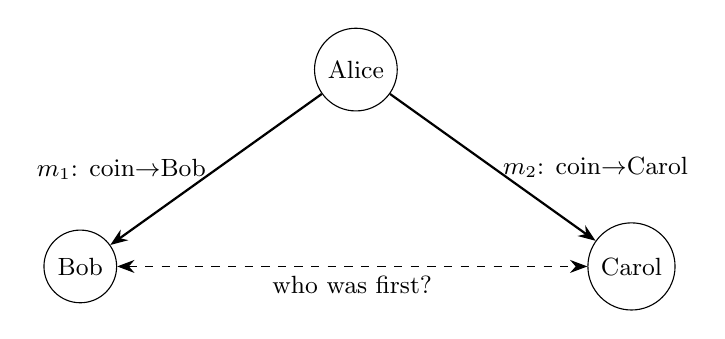
\begin{tikzpicture}
\node[node] (a) at (0,0) {Alice};
\node[node] (b) at (-3.5,-2.5) {Bob};
\node[node] (c) at (3.5,-2.5) {Carol};
\draw[->,thick] (a) -- node[left,font=\small]{$m_1$: coin$\to$Bob} (b);
\draw[->,thick] (a) -- node[right,font=\small]{$m_2$: coin$\to$Carol} (c);
\draw[dashed,<->] (b) -- node[below,font=\small]{who was first?} (c);
\end{tikzpicture}
\caption{Double spending: the two recipients cannot resolve the conflict locally.}
\end{figure}

\subsection{What exactly should the system achieve?}

\begin{plainenglish}
We want every honest participant to see the \emph{same} history of transactions, and we want new honest
transactions to get into that history within reasonable time. Two promises: \textbf{safety} (``what is
written down stays written down, for everyone'') and \textbf{liveness} (``honest transactions are not
blocked forever'').
\end{plainenglish}

\begin{formal}
\begin{definition}[Ledger / robust transaction ledger, Garay--Kiayias--Leonardos]\label{def:ledger}
Each honest party $P$ holds at every round $r$ a local chain $\mathcal C_P^r$. Its \emph{finalized ledger} $\mathsf{L}_P^r$ is that chain with the last $k$ blocks removed (the \emph{$k$-deep} prefix), flattened into a sequence of transactions. The protocol maintains a \emph{robust public transaction ledger} if:
\begin{itemize}[nosep]
\item \textbf{Persistence} (safety, parameter $k$): for all honest parties $P_1,P_2$ and rounds $r_1\le r_2$, the ledger $\mathsf{L}_{P_1}^{r_1}$ is a prefix of $\mathsf{L}_{P_2}^{r_2}$. In particular, if $P_1$ reports $\mathsf{tx}$ at position $i$ of its finalized ledger, every honest party reports $\mathsf{tx}$ at position $i$ from then on. The parameter $k$ is the number of \emph{confirmations} a transaction needs before it is treated as final.
\item \textbf{Liveness} (parameter $u$): if all honest parties try to include a valid transaction
$\mathsf{tx}$ for $u$ consecutive rounds, then $\mathsf{tx}$ appears in the finalized ledger of every
honest party.
\end{itemize}
Both properties are required to hold except with probability negligible in $k$ (and $u$).
\end{definition}
\end{formal}

\subsection{Threat model}

\begin{plainenglish}
A security claim means nothing unless we state \emph{who the attacker is}. For blockchains the key
questions are: (i) how much of the ``power'' (computing power or money) can the attacker control?
(ii) how slow or unreliable is the network, and can the attacker delay messages?
(iii) is the set of participants known (\emph{permissioned}) or can anyone join (\emph{permissionless})?
Bitcoin's remarkable feature is that it works in the permissionless setting, where identities are
free to create. Hence it counts \emph{computing power} instead of \emph{identities}.
\end{plainenglish}

\begin{formal}
We consider $n$ parties, of which an adversary $\Adv$ controls a fraction. Three axes:
\begin{description}[leftmargin=!,labelwidth=3.5cm]
\item[Resource.] $\Adv$ controls a fraction $q$ of total hash power (PoW) or stake (PoS); honest parties
control $p=1-q$.
\item[Network.] \emph{Synchronous}: messages are delivered within a known bound $\Delta$.
\emph{Partially synchronous}: the bound $\Delta$ exists but is unknown, or only holds after an unknown
global stabilisation time. \emph{Asynchronous}: no bound.
\item[Corruption.] \emph{Static} or \emph{adaptive} corruption; \emph{Byzantine} (arbitrary) behaviour.
\end{description}
\end{formal}

\begin{exercisebox}
\begin{enumerate}[nosep]
\item Explain why a purely signature-based scheme (no ordering) cannot prevent double spending.
\item Why is ``count identities'' ($1$ identity $=1$ vote) insecure in a permissionless system?
(This is a \emph{Sybil attack}.)
\item In Definition~\ref{def:ledger}, what happens to persistence if $k=0$? What trade-off does choosing a larger $k$ create for liveness and for the latency a merchant experiences?
\end{enumerate}
\end{exercisebox}
%================================================================
\section{Cryptographic Building Blocks}\label{sec:crypto}
%================================================================

\subsection{Hash functions}

\begin{plainenglish}
A cryptographic hash function is a ``digital fingerprint machine''. You feed in any file and out comes
a short, fixed-size fingerprint (256 bits for SHA-256). Three properties make fingerprints useful:
\begin{itemize}[nosep]
\item \textbf{Preimage resistance}: given a fingerprint, you cannot find any input producing it.
\item \textbf{Second-preimage resistance}: given one file, you cannot find a \emph{different} file with the same fingerprint.
\item \textbf{Collision resistance}: you cannot find \emph{any} two different files with the same fingerprint.
\end{itemize}
Blockchains use hashes everywhere: to link blocks, to summarise thousands of transactions, to build
addresses, and as the ``puzzle'' in mining.
\end{plainenglish}

\begin{formal}
Let $\Hash:\{0,1\}^*\to\{0,1\}^n$ (formally a keyed family $\{\Hash_s\}$ for the definitions to make sense).

\begin{definition}[Hash security notions]\label{def:hash}
For every PPT adversary $\Adv$ the following probabilities are $\negl(n)$:
\begin{align*}
\text{Preimage:}\quad & \Pr_{x\leftarrow_\$\{0,1\}^m}\big[\Adv(\Hash(x))=x' : \Hash(x')=\Hash(x)\big],\\
\text{2nd-preimage:}\quad & \Pr_{x\leftarrow_\$\{0,1\}^m}\big[\Adv(x)=x' : x'\neq x\wedge \Hash(x')=\Hash(x)\big],\\
\text{Collision:}\quad & \Pr\big[\Adv()=(x,x') : x\neq x'\wedge \Hash(x)=\Hash(x')\big].
\end{align*}
Collision resistance implies second-preimage resistance (and, for a compressing function, preimage resistance in a suitable sense).
\end{definition}

\begin{theorem}[Birthday bound]\label{thm:birthday}
If $\Hash$ behaves as a random function with $n$-bit output, an algorithm making $q$ hash evaluations
finds a collision with probability at most $\dfrac{q(q-1)}{2^{n+1}}$.
\end{theorem}
\begin{proof}
Let the evaluated (distinct) inputs be $x_1,\dots,x_q$ with outputs $y_i$ uniform and independent in
$\{0,1\}^n$. For each pair $i<j$, $\Pr[y_i=y_j]=2^{-n}$. By the union bound over the $\binom q2$ pairs,
$\Pr[\exists\, i<j: y_i=y_j]\le \binom q2 2^{-n}=\frac{q(q-1)}{2^{n+1}}$.
\end{proof}

\textbf{Random oracle model (ROM).} In proofs we often model $\Hash$ as a truly random function that every party can query
only through an oracle. It is an idealisation (no real hash function is a random oracle) but it is
the standard way to analyse Schnorr signatures, Bitcoin's PoW and Fiat--Shamir.
\end{formal}

\begin{exbox}[how big is $2^{128}$?]
For SHA-256, $n=256$, so a collision needs about $2^{128}$ evaluations. If the whole Bitcoin network
($\approx 10^{20}$ hashes per second, order of magnitude) worked on nothing else, it would produce
$\approx 3\times10^{27}$ hashes per year, which is only about $2^{91.4}$. Finding a SHA-256 collision by brute force would take
about $2^{36.6}\approx 10^{11}$ \emph{years}. With $q=2^{64}$ queries, Theorem~\ref{thm:birthday} gives probability at most
$2^{128}/2^{257}=2^{-129}$.
\end{exbox}

\begin{exbox}[avalanche effect]
Changing one character of the input changes about half the output bits, unpredictably. A 4-bit toy
hash would show \texttt{H(``tx1'')}$=\texttt{1011}$ but \texttt{H(``tx2'')}$=\texttt{0110}$. You cannot ``nudge'' a
fingerprint towards a target; this is exactly why mining is a lottery.
\end{exbox}

\subsection{Merkle trees}

\begin{plainenglish}
A block may contain thousands of transactions. Instead of putting them all inside the block header,
we compute \emph{one} fingerprint that commits to all of them: hash pairs of transactions, then
hash pairs of those hashes, and so on until one hash (the \textbf{root}) remains. The magic: to prove that
a particular transaction is in the block, you only need to show a handful of hashes (the
\emph{sibling} hashes on the path from the transaction to the root), not the whole block. Phone
wallets use this to verify payments without downloading the blockchain (``SPV'').
\end{plainenglish}

\begin{figure}[htbp]
\centering
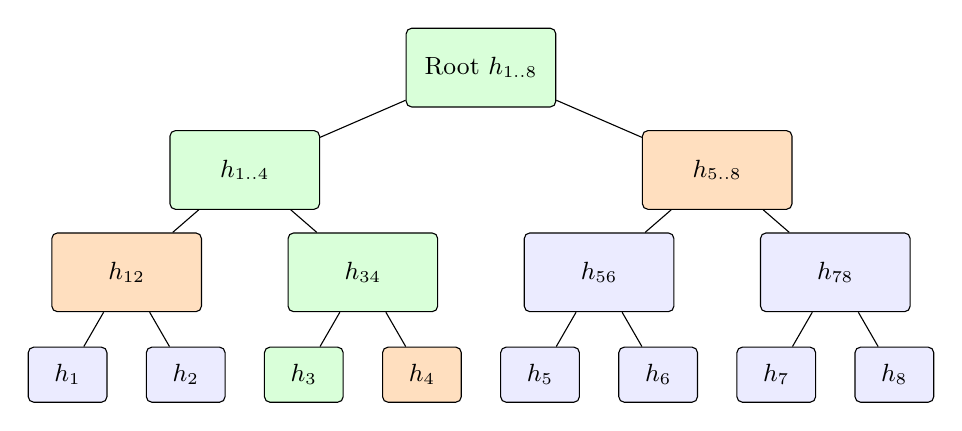
\begin{tikzpicture}[level distance=1.3cm,
  level 1/.style={sibling distance=6cm},
  level 2/.style={sibling distance=3cm},
  level 3/.style={sibling distance=1.5cm},
  every node/.style={font=\small}]
\node[blk,fill=green!15] (r) {Root $h_{1..8}$}
  child { node[blk,fill=green!15] (l) {$h_{1..4}$}
    child { node[blk,fill=orange!25] {$h_{12}$}
       child{node[blk,minimum width=1cm,minimum height=.7cm]{$h_1$}}
       child{node[blk,minimum width=1cm,minimum height=.7cm]{$h_2$}}}
    child { node[blk,fill=green!15] (x) {$h_{34}$}
       child{node[blk,minimum width=1cm,minimum height=.7cm,fill=green!15] (t3){$h_3$}}
       child{node[blk,minimum width=1cm,minimum height=.7cm,fill=orange!25]{$h_4$}}}}
  child { node[blk,fill=orange!25] {$h_{5..8}$}
    child { node[blk] {$h_{56}$}
       child{node[blk,minimum width=1cm,minimum height=.7cm]{$h_5$}}
       child{node[blk,minimum width=1cm,minimum height=.7cm]{$h_6$}}}
    child { node[blk] {$h_{78}$}
       child{node[blk,minimum width=1cm,minimum height=.7cm]{$h_7$}}
       child{node[blk,minimum width=1cm,minimum height=.7cm]{$h_8$}}}};
\end{tikzpicture}
\caption{Merkle tree over 8 transactions, with $h_i=\Hash(\mathsf{tx}_i)$ and $h_{ij}=\Hash(h_i\concat h_j)$ (the domain-separation tags of the definition below are omitted). To prove that $\mathsf{tx}_3$ is included, the verifier recomputes the green path from $h_3$ up to the root, using the three orange sibling hashes $h_4$, $h_{12}$ and $h_{5..8}$.}
\end{figure}

\begin{formal}
\begin{definition}[Merkle tree]
For leaves $x_1,\dots,x_N$ ($N=2^d$), define level-$0$ nodes $v_{0,i}=\Hash(0\concat x_i)$ and
$v_{\ell+1,i}=\Hash(1\concat v_{\ell,2i-1}\concat v_{\ell,2i})$. The root is $\mathsf{rt}=v_{d,1}$. A \emph{membership proof} for leaf $i$ is the
list of the $d$ sibling nodes along the path to the root; verification recomputes the path and compares with $\mathsf{rt}$.
(The prefixes $0,1$ are domain-separation tags that prevent leaf/internal-node confusion.)
\end{definition}

\begin{theorem}[Merkle binding]\label{thm:merkle}
If $\Hash$ is collision resistant, then no PPT adversary can output a root $\mathsf{rt}$ and two valid membership proofs
for \emph{different} values at the same position $i$, except with negligible probability.
The proof size is $d=\lceil\log_2 N\rceil$ hashes.
\end{theorem}
\begin{proof}
Suppose $\Adv$ outputs $\mathsf{rt}$ and valid proofs $\pi,\pi'$ for $x\neq x'$ at the same position $i$. The position fixes, at every level, whether the path node is a left or a right child, so the two verifications compute paths $v_0,v_1,\dots,v_d$ and $v_0',v_1',\dots,v_d'$ with $v_d=v_d'=\mathsf{rt}$.
If $v_0=v_0'$, then $\Hash(0\concat x)=\Hash(0\concat x')$ with $x\neq x'$ is a collision. Otherwise $v_0\neq v_0'$ while $v_d=v_d'$, so there is a smallest level $\ell\ge1$ with $v_\ell=v_\ell'$, and then $v_{\ell-1}\neq v_{\ell-1}'$. Level $\ell$ is computed as $\Hash(1\concat a\concat b)$ resp.\ $\Hash(1\concat a'\concat b')$, where $v_{\ell-1}$ (resp.\ $v_{\ell-1}'$) occupies the same side in both and the other entry is the sibling supplied by the proof. As $v_{\ell-1}\ne v_{\ell-1}'$ we have $(a,b)\neq(a',b')$, yet the hashes agree: a collision. Hence a successful $\Adv$ yields a collision finder with the same running time. \qedhere
\end{proof}
\end{formal}

\begin{exbox}[verifying a Merkle proof]\label{ex:merkleproof}
Block with 8 transactions; you hold $\mathsf{tx}_3$ and the root $\mathsf{rt}$. The full node sends the proof
$(h_4,\ h_{12},\ h_{5..8})$ together with left/right flags. You compute
$h_3=\Hash(\mathsf{tx}_3)$, then $h_{34}=\Hash(h_3\concat h_4)$, then $h_{1..4}=\Hash(h_{12}\concat h_{34})$, then
$\mathsf{rt}'=\Hash(h_{1..4}\concat h_{5..8})$, and accept iff $\mathsf{rt}'=\mathsf{rt}$. You hashed $4$ times and received
$3$ hashes ($96$ bytes) instead of $8$ transactions. For a block with $4000$ transactions
you need only $\lceil\log_2 4000\rceil=12$ hashes ($384$ bytes).
\end{exbox}

\begin{warnbox}
Bitcoin duplicates the last node when the number of nodes at a level is odd. The famous consequence (CVE-2012-2459) is that two
different transaction lists can have the same Merkle root (Figure~\ref{fig:merkledup}). Domain-separation and careful handling of odd levels
are not cosmetic details.
\end{warnbox}

\begin{figure}[htbp]
\centering
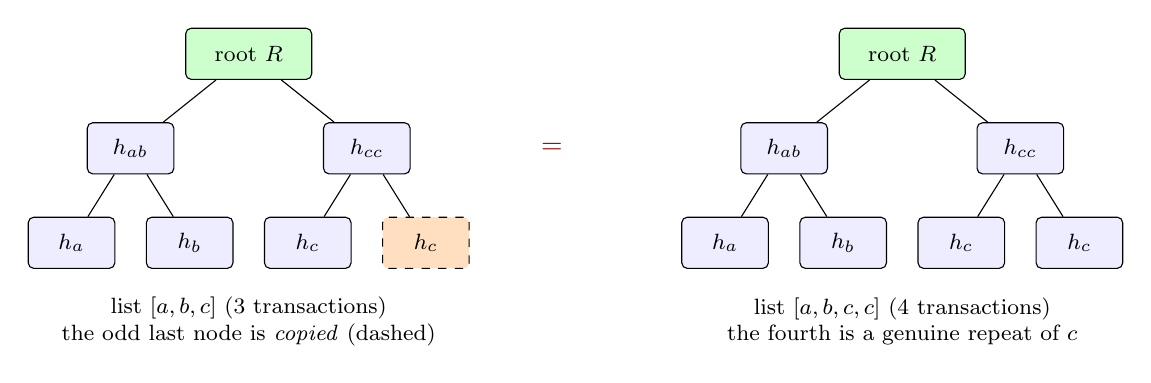
\begin{tikzpicture}[font=\footnotesize,
 n/.style={draw,rounded corners=2pt,minimum width=1.1cm,minimum height=0.65cm,fill=blue!7,align=center},
 d/.style={n,dashed,fill=orange!25}]
\begin{scope}
\node[n] (a1) at (0,0) {$h_a$}; \node[n] (b1) at (1.5,0) {$h_b$}; \node[n] (c1) at (3,0) {$h_c$}; \node[d] (c1d) at (4.5,0) {$h_c$};
\node[n] (ab1) at (0.75,1.2) {$h_{ab}$}; \node[n] (cc1) at (3.75,1.2) {$h_{cc}$};
\node[n,fill=green!20,minimum width=1.6cm] (r1) at (2.25,2.4) {root $R$};
\draw (a1)--(ab1) (b1)--(ab1) (c1)--(cc1) (c1d)--(cc1) (ab1)--(r1) (cc1)--(r1);
\node[align=center] at (2.25,-1.0) {list $[a,b,c]$ (3 transactions)\\ the odd last node is \emph{copied} (dashed)};
\end{scope}
\begin{scope}[xshift=8.3cm]
\node[n] (a2) at (0,0) {$h_a$}; \node[n] (b2) at (1.5,0) {$h_b$}; \node[n] (c2) at (3,0) {$h_c$}; \node[n] (c2d) at (4.5,0) {$h_c$};
\node[n] (ab2) at (0.75,1.2) {$h_{ab}$}; \node[n] (cc2) at (3.75,1.2) {$h_{cc}$};
\node[n,fill=green!20,minimum width=1.6cm] (r2) at (2.25,2.4) {root $R$};
\draw (a2)--(ab2) (b2)--(ab2) (c2)--(cc2) (c2d)--(cc2) (ab2)--(r2) (cc2)--(r2);
\node[align=center] at (2.25,-1.0) {list $[a,b,c,c]$ (4 transactions)\\ the fourth is a genuine repeat of $c$};
\end{scope}
\node[font=\bfseries,red!60!black] at (6.1,1.2) {$=$};
\end{tikzpicture}
\caption{Duplicating the last node on odd levels (Bitcoin's rule) gives two different transaction lists the \emph{same} Merkle root: the ambiguity behind CVE-2012-2459. Hashing the number of leaves into the root, or never duplicating, removes it.}
\label{fig:merkledup}
\end{figure}

\subsection{Digital signatures}

\begin{plainenglish}
A signature is the digital analogue of a handwritten signature, but it is tied to the \emph{content}
of the message. Alice has a secret key she never shares and a public key everyone knows. Only Alice can produce a signature
on ``pay Bob 5 coins'', yet everyone can check it. In a blockchain, \emph{owning coins means knowing a secret key}; spending coins means signing.
\end{plainenglish}

\begin{formal}
\begin{definition}[Signature scheme]
A triple $(\KeyGen,\Sign,\Verify)$: $\KeyGen(1^\lambda)\to(\sk,\pk)$; $\Sign(\sk,m)\to\sigma$; $\Verify(\pk,m,\sigma)\to\{0,1\}$,
with correctness $\Verify(\pk,m,\Sign(\sk,m))=1$.
\end{definition}

\begin{definition}[EUF-CMA]
The adversary receives $\pk$ and access to a signing oracle $\Sign(\sk,\cdot)$. It wins if it outputs $(m^*,\sigma^*)$ with
$\Verify(\pk,m^*,\sigma^*)=1$ and $m^*$ was never queried. The scheme is EUF-CMA secure if every PPT adversary wins with negligible probability.
\end{definition}

\textbf{RSA signatures.} In RSA signatures, signing is the ``decryption'' operation and verifying is the ``encryption'' operation.

\begin{plainenglish}
In RSA you have a public pair $(n,e)$ and a secret exponent $d$. To \emph{encrypt}, anyone raises the message to the power $e$; only the key holder can undo this with $d$. For \emph{signing} we run the machine backwards: the key holder raises the message to the power $d$ (something only she can do) and anyone can check the result by raising it to the power $e$ and seeing whether the original message comes back. A valid signature is therefore a number that ``only the owner of $d$ could have produced''.

There is one trap: signing the raw message is \emph{insecure}. Signatures can be combined and invented (see below). The cure is to first hash the message and sign the hash: \textbf{hash-then-sign}, formalised as the \emph{full-domain hash} (RSA-FDH).
\end{plainenglish}

\begin{formal}
Let $n=pq$ with large primes $p,q$, $e$ coprime to $\varphi(n)=(p-1)(q-1)$, and $d\equiv e^{-1}\pmod{\varphi(n)}$. Let $\Hash:\{0,1\}^*\to\Z_n^*$ (a ``full-domain'' hash, modelled as a random oracle).
\begin{itemize}[nosep]
\item $\KeyGen$: $\sk=(n,d)$, $\pk=(n,e)$. \quad $\Sign(\sk,m)$: $\sigma=\Hash(m)^d\bmod n$. \quad $\Verify(\pk,m,\sigma)$: accept iff $\sigma^e\equiv\Hash(m)\pmod n$.
\end{itemize}
\begin{proposition}[Correctness]
$\sigma^e=\Hash(m)^{ed}=\Hash(m)^{1+k\varphi(n)}\equiv\Hash(m)\pmod n$ by Euler's theorem.
\end{proposition}

\begin{theorem}[Bellare--Rogaway~\cite{BR93}; Coron~\cite{Coron00}]
In the random oracle model, RSA-FDH is EUF-CMA secure under the RSA assumption (given $(n,e,y)$ with $y\leftarrow_\$\Z_n^*$, it is hard to find $x$ with $x^e\equiv y$).
\end{theorem}
\begin{proof}[Proof sketch]
Given an RSA challenge $(n,e,y)$ and a forger making $q_H$ hash queries, the reduction guesses an index $j\in[q_H]$ and simulates the oracle: for query $i\ne j$ it picks $s_i\leftarrow_\$\Z_n^*$ and answers $\Hash(m_i)=s_i^e$, remembering $s_i$; for query $j$ it answers $\Hash(m_j)=y$. A signing query on $m_i$ ($i\neq j$) is answered with $s_i$, which is a valid signature because $s_i^e=\Hash(m_i)$. All answers are uniform, so the simulation is perfect. If the forger outputs a valid forgery $\sigma^*$ on $m^*=m_j$ (probability $\ge\epsilon/q_H$), then $(\sigma^*)^e=y$ and the reduction has inverted RSA. Coron's refinement loses only a factor $q_S$ (number of signing queries) rather than $q_H$ by answering a random subset of queries with $s_i^e$ and the rest with $y\,s_i^e$.
\end{proof}
\end{formal}

\begin{exbox}[toy RSA-FDH]
Take $p=5$, $q=11$, so $n=55$ and $\varphi(n)=40$. Choose $e=3$; then $d=27$ since $3\cdot27=81\equiv1\pmod{40}$.
Suppose $\Hash(m)=12$ for the message $m=\text{``pay Bob 5''}$ (a toy hash). \emph{Sign}: $\sigma=12^{27}\bmod55$. Modulo $5$: $12\equiv2$ and $2^{27}=2^{27\bmod4}=2^3=8\equiv3$. Modulo $11$: $12\equiv1$, so $1$. The Chinese remainder theorem gives $\sigma=23$.
\emph{Verify}: $23^3=12167=55\cdot221+12\equiv12=\Hash(m)$ \checkmark.
\end{exbox}

\begin{exbox}[why textbook RSA, with no hash, is forgeable]
Without the hash, the signature on a number $h$ is $\sigma(h)=h^d$. With the same toy key:
\begin{itemize}[nosep]
\item \emph{Multiplicative forgery}: $\sigma(2)=18$ and $\sigma(3)=42$ are signatures a victim produced. Then $18\cdot42=756\equiv41$ is a valid signature on $2\cdot3=6$, a message the victim never signed. Indeed $41^3\equiv6\pmod{55}$.
\item \emph{Existential forgery without the key}: pick any $\sigma=7$ and compute $m=\sigma^e=343\equiv13$. Then $(m,\sigma)=(13,7)$ verifies, though nobody signed $13$.
\end{itemize}
Hashing breaks both attacks: the attacker would have to produce $\sigma$ for $\Hash(m)$, and $\Hash(m_1)\Hash(m_2)\neq\Hash(m_1m_2)$ for a one-way hash.
\end{exbox}

\begin{warnbox}[(parameters matter)]
Textbook examples use tiny primes; real RSA needs $n$ of at least $2048$ bits. Standardised padding (RSASSA-PSS, PKCS\#1~v1.5) replaces the idealised full-domain hash in practice.
\end{warnbox}

\begin{plainenglish}
\textbf{Why does Bitcoin not simply use RSA?} The scheme is secure, but it is expensive on a blockchain, where every node stores every signature forever. A 2048-bit RSA signature is $256$ bytes, four times larger than a $64$-byte Schnorr signature at a comparable $\approx112$--$128$-bit security level; keys are $256$ bytes versus $32$. Elliptic-curve and discrete-log signatures are also easier to aggregate and to split among several signers (Part~8). Finally, RSA key generation (finding large primes) is slow and awkward for wallets.
\end{plainenglish}

\begin{exbox}[cost on a blockchain]
A block of $1$ MB with simple one-input transactions of about $250$ bytes using $64$-byte signatures holds roughly $4000$ transactions. Replace the signature and the public key by RSA-2048 ones (a $256$-byte signature instead of $64$ bytes and a $256$-byte key instead of $32$ bytes, adding about $192+224=416$ bytes), the transaction becomes about $670$ bytes and the block holds only about $1500$ transactions: a drop of roughly $60\%$ in throughput at a similar security level.
\end{exbox}

\textbf{Schnorr signatures.} Let $\G=\langle g\rangle$ be a group of prime order $q$ in which discrete log is hard, and $\Hash:\{0,1\}^*\to\Z_q$ a random oracle.
\begin{itemize}[nosep]
\item $\KeyGen$: $x\leftarrow_\$\Z_q$, $\sk=x$, $\pk=y=g^x$.
\item $\Sign(x,m)$: $r\leftarrow_\$\Z_q$; $R=g^r$; $c=\Hash(R\concat \pk\concat m)$; $s=r+cx \bmod q$; output $\sigma=(R,s)$ (or $(c,s)$).
\item $\Verify(y,m,(R,s))$: $c=\Hash(R\concat y\concat m)$; accept iff $g^s=R\cdot y^c$.
\end{itemize}

\begin{proposition}[Correctness]
$g^s=g^{r+cx}=g^r(g^x)^c=R\,y^c$.
\end{proposition}

\begin{theorem}[Pointcheval--Stern~\cite{PS96}, informal]
In the random oracle model, Schnorr signatures are EUF-CMA secure under the discrete-logarithm assumption in $\G$.
\end{theorem}
\emph{Proof idea (forking lemma).} Run the forger twice with identical randomness up to the query $\Hash(R\concat y\concat m)$, and answer that query with different values $c\neq c'$. If both runs succeed
you obtain $g^{s}=Ry^{c}$ and $g^{s'}=Ry^{c'}$, hence $g^{s-s'}=y^{c-c'}$, so $x=(s-s')(c-c')^{-1}\bmod q$: the forger has solved discrete log. The forking lemma says the two runs both succeed
with probability roughly $\epsilon^2/q_H$ if the forger succeeds with probability $\epsilon$ and makes $q_H$ random oracle queries.
\end{formal}

\begin{exbox}[Schnorr step by step with tiny numbers]\label{ex:schnorr}
\medskip\noindent\textbf{The cast of characters.}
\begin{center}\small
\begin{tabular}{@{}cp{5.2cm}p{5.8cm}@{}}
\toprule
Symbol & Meaning & Who knows it\\
\midrule
$p,\ q,\ g$ & public ``playground'': we compute modulo the prime $p$; $g$ is a number whose powers cycle through exactly $q$ values & everybody\\
$x$ & \textbf{private key}, a secret number between $0$ and $q-1$ & only the signer\\
$y=g^x$ & \textbf{public key} & everybody\\
$m$ & the message (here ``pay Bob 5'') & everybody\\
$r$ & one-time secret random number (the \emph{nonce}); thrown away after signing & only the signer\\
$R=g^r$ & public ``commitment'' to $r$ & everybody (part of the signature)\\
$c$ & \textbf{challenge}: a number computed by hashing $(R,y,m)$ & everybody\\
$s=r+c\cdot x$ & \textbf{response}; with $R$ forms the signature $(R,s)$ & everybody\\
\bottomrule
\end{tabular}
\end{center}

\noindent\textbf{Step 0: the playground.} Work with numbers modulo $p=23$ (``modulo'' means we keep only the remainder after dividing by $23$). Pick $g=4$. Its powers modulo $23$ are:
\begin{center}\small
\begin{tabular}{@{}c|ccccccccccc@{}}
exponent $e$ & 1&2&3&4&5&6&7&8&9&10&11\\
\hline
$4^e \bmod 23$ & 4&16&18&3&12&2&8&9&13&6&1\\
\end{tabular}
\end{center}
After $q=11$ steps we are back to $1$, so the powers of $4$ repeat with period $11$. Hence \emph{exponents can be reduced modulo $11$}: $4^{26}=4^{26\bmod 11}=4^4$. This table is our whole ``discrete-log oracle'': because the numbers are tiny, we can look up that $4^3=18$. For a $256$-bit group no such table exists, and finding $e$ from $4^e$ is the infeasible discrete-logarithm problem.

\medskip\noindent\textbf{Step 1: key generation.} The signer picks the private key $x=3$. The public key is $y=g^x=4^3=18$ (from the table). The signer publishes $y=18$ and keeps $x=3$ secret.

\medskip\noindent\textbf{Step 2: signing the message $m=$ ``pay Bob 5''.}
\begin{enumerate}[nosep]
\item Pick a fresh random nonce, say $r=5$. Compute $R=g^r=4^5=12$.
\item Compute the challenge $c=\Hash(R\concat y\concat m)\bmod 11$. A real hash is unpredictable, so for the example just suppose it returns $c=7$.
\item Compute the response $s=r+c\cdot x \bmod 11=5+7\cdot3=26\equiv4 \pmod{11}$.
\item The signature is $(R,s)=(12,4)$. Throw $r$ away.
\end{enumerate}

\medskip\noindent\textbf{Step 3: verification.} Anyone who knows $y=18$, $m$ and the signature $(12,4)$:
\begin{enumerate}[nosep]
\item Recompute $c=\Hash(R\concat y\concat m)=7$ (same hash, same inputs).
\item Left side: $g^s=4^4=3$.
\item Right side: $R\cdot y^c=12\cdot18^7$. Since $18=4^3$, we have $18^7=4^{21}=4^{21\bmod11}=4^{10}=6$, so $R\cdot y^c=12\cdot6=72\equiv3\pmod{23}$.
\item Both sides equal $3$: \textbf{accept}.
\end{enumerate}

\noindent\textbf{Why the check works (look at the exponents).} Write everything as a power of $4$: $R=4^{r}$ and $y^c=4^{xc}$, so $R\cdot y^c=4^{r+xc}$, which is exactly $4^s$. The verifier never sees $x$ or $r$ but can check ``$s=r+cx$'' \emph{in the exponent}. In our numbers: $4^5\cdot4^{21}=4^{26}=4^{4}$.

\medskip\noindent\textbf{What if the message is changed?} Suppose an attacker changes the message to ``pay Bob 500''. The hash now gives a different challenge, say $c'=8$. The check becomes $g^s=3$ against $R\cdot y^{8}=12\cdot4^{24}=12\cdot4^{2}=12\cdot16=192\equiv8\pmod{23}$. Since $3\ne8$: \textbf{reject}. The signature is bound to the exact message (and to $R$ and $y$) through $c$.

\medskip\noindent\textbf{Can an observer recover $x$?} They see $y=18$, $R=12$, $s=4$ and $c=7$. The signature satisfies $4=r+7x\pmod{11}$: \emph{one equation, two unknowns}. Every candidate $x\in\{0,\dots,10\}$ gives some $r=4-7x\bmod11$ that fits (for $x=0$: $r=4$; for $x=3$: $r=5$; for $x=7$: $r=10$, \dots). Only the extra fact $R=4^r$ would single out the right pair, and that needs the discrete log of $R$, easy here via the table ($4^5=12\Rightarrow r=5$) but infeasible in a real group. This is why the nonce $r$ must be secret and random.

\medskip\noindent\textbf{What goes wrong if the nonce is reused?} Sign a second message $m_2$ with the \emph{same} $r=5$ (so the same $R=12$). Suppose its challenge is $c_2=2$. Then $s_2=5+2\cdot3=11\equiv0$. An attacker now holds $s_1=4$ and $s_2=0$ with known $c_1=7$, $c_2=2$:
$$s_1-s_2=(c_1-c_2)\,x\ \Rightarrow\ 4=5x\pmod{11}\ \Rightarrow\ x=4\cdot5^{-1}=4\cdot9=36\equiv3.$$
(Here $5^{-1}=9$ because $5\cdot9=45\equiv1\pmod{11}$.) The private key $x=3$ is revealed.

\medskip\noindent\textbf{Cheating without the key?} Without $x$, a forger could just guess $s$ and hope: with $q=11$ she is right with probability $1/11\approx9\%$. With the real $q\approx2^{256}$ the chance is $2^{-256}$.

\medskip\noindent\textbf{Compare with Diffie--Hellman key exchange.} The two use the same ingredients: the same kind of group, public values of the form $g^{\text{secret}}$, and the same hardness assumption (discrete log).
\begin{center}\small
\begin{tabular}{@{}p{3.1cm}p{5.5cm}p{5.5cm}@{}}
\toprule
 & \textbf{Diffie--Hellman} & \textbf{Schnorr signature}\\
\midrule
Goal & two parties agree on a shared secret key & the signer proves ``I know $x$'' and binds the proof to a message\\
Public values & $A=g^a$, $B=g^b$ & $y=g^x$ (long-term), $R=g^r$ (one-time)\\
Result & $K=g^{ab}=B^a=A^b$ & check $g^s=R\cdot y^c$\\
Secret needed & each party keeps $a$ or $b$ & signer keeps $x$ and uses a fresh $r$ per signature\\
Interaction & two parties exchange values & non-interactive: only the signer acts, anybody verifies\\
\bottomrule
\end{tabular}
\end{center}
You can think of Schnorr as follows: $R=g^r$ is a one-time ``DH public key'' of the signer, and the challenge $c$ is made by hashing instead of being sent by a verifier. The check $g^s=R\,y^c$ then says that the exponent of $R$ combined with $c$ times the exponent of $y$ is what the signer claims.

\medskip\noindent\textbf{Where does the hash come from? (interactive view).} Imagine a live protocol: (1) the prover sends $R=g^r$; (2) the verifier sends a random challenge $c$; (3) the prover answers $s=r+cx$; the verifier checks $g^s=R\,y^c$. A signature is this protocol with the verifier replaced by a hash function that produces $c=\Hash(R\concat y\concat m)$ (the \emph{Fiat--Shamir transform}). Putting $m$ into the hash is what makes it a signature on $m$.

\medskip\noindent(For real use, $p$ and $q$ are $256$-bit numbers, not $23$ and $11$.)
\end{exbox}

\begin{figure}[htbp]
\centering
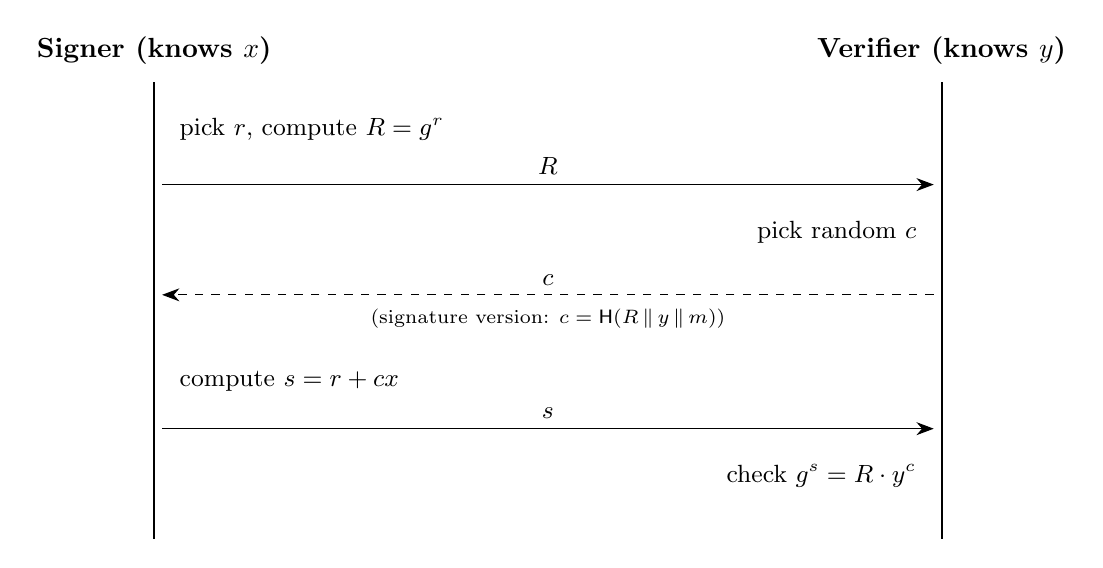
\begin{tikzpicture}[x=1cm,y=1cm]
\node[font=\bfseries] at (0,0) {Signer (knows $x$)};
\node[font=\bfseries] at (10,0) {Verifier (knows $y$)};
\draw[thick] (0,-0.4)--(0,-6.2); \draw[thick] (10,-0.4)--(10,-6.2);
\node[font=\small,anchor=west] at (0.2,-1) {pick $r$, compute $R=g^r$};
\draw[->] (0.1,-1.7)--node[above,font=\small]{$R$}(9.9,-1.7);
\node[font=\small,anchor=east] at (9.8,-2.3) {pick random $c$};
\draw[->,dashed] (9.9,-3.1)--node[above,font=\small]{$c$}(0.1,-3.1);
\node[font=\scriptsize,anchor=north] at (5,-3.15) {(signature version: $c=\Hash(R\concat y\concat m)$)};
\node[font=\small,anchor=west] at (0.2,-4.2) {compute $s=r+cx$};
\draw[->] (0.1,-4.8)--node[above,font=\small]{$s$}(9.9,-4.8);
\node[font=\small,anchor=east] at (9.8,-5.4) {check $g^s=R\cdot y^c$};
\end{tikzpicture}
\caption{The Schnorr identification protocol (solid and dashed arrows). In the signature version the dashed message is replaced by a hash computed by the signer, so no interaction is needed.}
\end{figure}

\begin{warnbox}[(nonce reuse)]
If the same $r$ is used for two messages, then $s_1-s_2=(c_1-c_2)x$ and the private key is recovered immediately.
Exactly this happened to ECDSA implementations with bad randomness (\eg\ Android wallets, 2013, and the PlayStation~3 signing key), and coins were stolen.
\end{warnbox}

\textbf{ECDSA and Bitcoin.} Bitcoin originally used ECDSA over the curve \texttt{secp256k1} (group order $\approx2^{256}$, $128$-bit security). ECDSA is the elliptic-curve version of DSA, an ElGamal-type scheme designed in part to avoid the (now expired) Schnorr patent. It needs a modular inversion when signing, its security proofs require idealised or modified assumptions, and its verification equation is not linear in the secret key, so it does not aggregate or threshold easily.
Since the 2021 \emph{Taproot} upgrade Bitcoin also supports Schnorr signatures (BIP-340~\cite{BIP340}), which enable key/signature aggregation (revisited in Part~8).

\begin{exercisebox}
\begin{enumerate}[nosep]
\item With $n=64$ bits of hash output, how many evaluations give $50\%$ collision probability (approximately)? Use $q\approx1.18\cdot2^{n/2}$.
\item Build the Merkle tree for 5 leaves in a way that avoids the Bitcoin duplication ambiguity. Show two different leaf lists that collide under the Bitcoin rule (Figure~\ref{fig:merkledup}).
\item Redo Example~\ref{ex:schnorr} with $x=4$, $r=2$, $c=9$.
\item Prove that if the same nonce $r$ is used for two different messages, the Schnorr secret key is leaked.
\item Show that collision resistance implies second-preimage resistance.
\item Using the toy key $n=55,e=3,d=27$, sign $\Hash(m)=7$, verify the signature, and forge a signature on $7\cdot12=84\equiv29$ from signatures on $7$ and $12$ (textbook RSA).
\item Show that if an attacker obtains $\sigma(h_1)$ and $\sigma(h_2)$ for textbook RSA, she can sign $h_1h_2^{-1}\bmod n$ as well.
\end{enumerate}
\end{exercisebox}
%================================================================
\section{Bitcoin in Detail}\label{sec:bitcoin}
%================================================================

\subsection{The UTXO model}

\begin{plainenglish}
Bitcoin does not keep account balances. Instead it tracks \emph{unspent transaction outputs} (UTXOs), which are like individual banknotes of various denominations.
A transaction destroys some banknotes (its \emph{inputs}) and creates new ones (its \emph{outputs}). If you hold a 50-coin note and
want to pay 30, you spend the 50 note, create a 30 note for the payee and a ``change'' note of nearly 20 for yourself;
the small leftover is the miner's \textbf{fee}. Your ``balance'' is simply the sum of the notes you can sign for.
\end{plainenglish}

\begin{figure}[htbp]
\centering
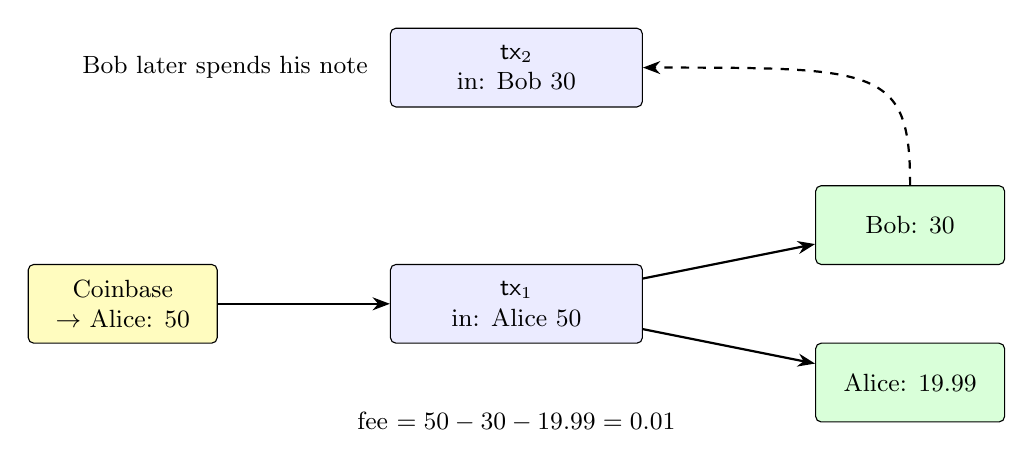
\begin{tikzpicture}[x=1cm,y=1cm]
\node[blk,minimum width=2.4cm,fill=yellow!25] (cb) at (0,0) {Coinbase\\ $\to$ Alice: 50};
\node[blk,minimum width=3.2cm] (t1) at (5,0) {$\mathsf{tx}_1$\\ in: Alice 50};
\node[blk,minimum width=2.4cm,fill=green!15] (o1) at (10,1) {Bob: 30};
\node[blk,minimum width=2.4cm,fill=green!15] (o2) at (10,-1) {Alice: 19.99};
\node[font=\small] at (5,-1.5) {fee $=50-30-19.99=0.01$};
\node[blk,minimum width=3.2cm] (t2) at (5,3) {$\mathsf{tx}_2$\\ in: Bob 30};
\draw[->,thick] (cb) -- (t1);
\draw[->,thick] (t1) -- (o1);
\draw[->,thick] (t1) -- (o2);
\draw[->,thick,dashed] (o1.north) .. controls +(0,1.5) and +(3,0) .. (t2.east);
\node[font=\small] at (1.3,3) {Bob later spends his note};
\end{tikzpicture}
\caption{A UTXO transaction graph. Outputs are consumed exactly once.}
\end{figure}

\begin{formal}
\begin{definition}[Transaction]
A transaction $\mathsf{tx}=(\mathsf{In},\mathsf{Out})$ where each input is a pointer $(\mathsf{txid},j)$ to the $j$-th output of an earlier transaction plus an unlocking script (typically a signature and public key), and each output is a pair $(v,\mathsf{lock})$ of an amount and a locking script.
\end{definition}
\begin{definition}[Validity]
$\mathsf{tx}$ is valid w.r.t.\ UTXO set $U$ if (i) every input references an output in $U$ (this stops double spending), (ii) every unlocking script satisfies the referenced locking script, (iii) no input is referenced twice, and (iv) $\sum_{\text{in}} v\ge\sum_{\text{out}} v$.
The fee is $\sum_{\text{in}} v-\sum_{\text{out}} v$. After inclusion, $U\leftarrow (U\setminus\text{inputs})\cup\text{outputs}$.
\end{definition}
\end{formal}

\begin{exbox}[UTXO bookkeeping]
Initial $U=\{A_1{=}50\}$ owned by Alice. $\mathsf{tx}_1$ spends $A_1$, creating $B_1{=}30$ (Bob) and $A_2{=}19.99$ (Alice).
Now $U=\{B_1,A_2\}$. If Alice tries to spend $A_1$ again, condition (i) fails because $A_1\notin U$.
Alice cannot list $A_2$ twice as an input of the same transaction (iii), and cannot create outputs worth more than inputs (iv).
\end{exbox}

\subsection{Script: programmable locks}

\begin{plainenglish}
Each output carries a tiny program (a \emph{locking script}) and each input supplies a matching program (an \emph{unlocking script}). The money moves only if the combined program ends with ``true''. The
most common lock, \textbf{Pay-to-Public-Key-Hash (P2PKH)}, says: ``show me a public key that hashes to this address, and a valid signature from it''. Hiding the public key behind a hash has a nice
side-effect: until you spend, only the hash is public (relevant for quantum attacks in Part~8).
\end{plainenglish}

\begin{exbox}[stack execution of P2PKH]
Locking script: \texttt{OP\_DUP OP\_HASH160 <addr> OP\_EQUALVERIFY OP\_CHECKSIG}. Unlocking script: \texttt{<sig> <pk>}.
\begin{center}\small
\begin{tabular}{@{}lll@{}}
\toprule
Step & Operation & Stack (top on the right)\\
\midrule
1 & push \texttt{sig}, push \texttt{pk} & \texttt{sig, pk}\\
2 & \texttt{OP\_DUP} & \texttt{sig, pk, pk}\\
3 & \texttt{OP\_HASH160} & \texttt{sig, pk, H(pk)}\\
4 & push \texttt{<addr>} & \texttt{sig, pk, H(pk), addr}\\
5 & \texttt{OP\_EQUALVERIFY} (abort if unequal) & \texttt{sig, pk}\\
6 & \texttt{OP\_CHECKSIG} & \texttt{true}\\
\bottomrule
\end{tabular}
\end{center}
\texttt{OP\_HASH160} computes $\mathrm{RIPEMD160}(\mathrm{SHA256}(\cdot))$; the address is this $160$-bit hash (written with a version prefix and checksum).
\end{exbox}

Script is deliberately \emph{not} Turing complete (no loops), so every script terminates and validation cost is bounded.

\subsection{Blocks and the chain}

\begin{plainenglish}
Transactions are grouped into \textbf{blocks}. Each block header contains the hash of the previous block header, so the blocks form a chain. If anyone alters an old block, its hash changes,
so the next block's ``previous hash'' field no longer matches, and so on up the chain: tampering is \emph{visible}. To make tampering also \emph{expensive}, each block must carry a proof of
work (next section).
\end{plainenglish}

\begin{figure}[htbp]
\centering
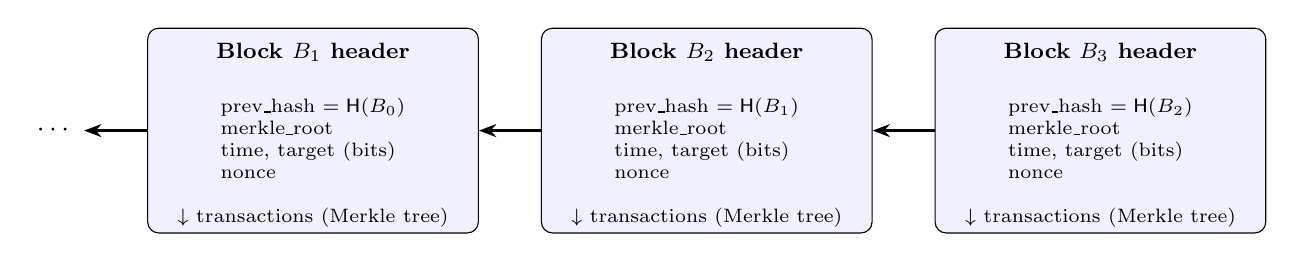
\begin{tikzpicture}[node distance=0.9cm]
\foreach \i/\x in {1/0,2/5,3/10}{
  \node[draw,rounded corners,minimum width=4.2cm,minimum height=2.6cm,fill=blue!6] (b\i) at (\x,0) {};
  \node[font=\footnotesize\bfseries] at (\x,1.0) {Block $B_\i$ header};
  \node[font=\scriptsize,align=left] at (\x,-0.1) {prev\_hash $=\Hash(B_{\the\numexpr\i-1\relax})$\\ merkle\_root\\ time, target (bits)\\ nonce};
  \node[font=\scriptsize] at (\x,-1.1) {$\downarrow$ transactions (Merkle tree)};
}
\draw[->,thick] (b2.west) -- (b1.east);
\draw[->,thick] (b3.west) -- (b2.east);
\draw[->,thick] (b1.west) -- ++(-0.8,0) node[left]{$\cdots$};
\end{tikzpicture}
\caption{The chain: each header commits to its predecessor and to its transactions.}
\end{figure}

The 80-byte Bitcoin header has fields: version (4 B), previous block hash (32 B), Merkle root (32 B), timestamp (4 B), compact target \texttt{nBits} (4 B), nonce (4 B). The \emph{block ID} is
$\Hash(\Hash(\text{header}))$ with $\Hash=$ SHA-256.

\subsection{Proof of work}

\begin{plainenglish}
Anyone can propose the next block, so who gets to? Bitcoin runs a \emph{lottery weighted by computing power}. Miners repeatedly change a counter (the nonce) in the header and hash it, hoping the result is a
number below a \textbf{target}, i.e.\ a hash starting with many zeros. There is no shortcut: each attempt is an independent coin flip. A miner who owns 10\% of all hash power wins about 10\% of the lotteries.
Winning is easy to verify (one hash) but hard to achieve (trillions of hashes). This makes \emph{rewriting history} cost real energy.
\end{plainenglish}

\begin{formal}
\begin{definition}[PoW puzzle]
Given a header $h$ (containing $\mathsf{prev}$, Merkle root, etc.) and target $T\in\{0,\dots,2^{256}-1\}$, find a nonce $\eta$ such that $\Hash(h\concat\eta)<T$.
Treating $\Hash$ as a random oracle, each attempt succeeds independently with probability $p_T=\dfrac{T}{2^{256}}$.
\end{definition}

\begin{theorem}[Block discovery is memoryless]\label{thm:expo}
Let the network perform $\mu$ hashes per second and success probability per hash be $p_T$. The number of hashes until the first success is geometric with mean $1/p_T$, and as $p_T\to0$ the
waiting time (in seconds) converges to an exponential random variable with rate $\mu p_T$. Hence the block interval has mean $1/(\mu p_T)$, and the block arrival process is a Poisson process.
\end{theorem}
\begin{proof}
$\Pr[\text{first success at attempt }k]=(1-p_T)^{k-1}p_T$, so the number of attempts $N$ is geometric with $\E[N]=1/p_T$. In time $t$ the miner makes $\mu t$ attempts, so
$\Pr[\text{no success by }t]=(1-p_T)^{\mu t}=\exp\!\big(\mu t\ln(1-p_T)\big)\to e^{-\mu p_T t}$ as $p_T\to0$ (using $\ln(1-p_T)\approx-p_T$).
This is the CDF complement of an exponential distribution with rate $\lambda=\mu p_T$.
\end{proof}

\begin{corollary}[Hash power equals winning probability]
If miner $i$ has hash rate $\mu_i$ and $\mu=\sum_j\mu_j$, then the probability that $i$ finds the next block is $\mu_i/\mu$.
\end{corollary}
\begin{proof}
Independent exponentials with rates $\lambda_i=\mu_ip_T$: $\Pr[\text{$i$ is minimum}]=\lambda_i/\sum_j\lambda_j$.
\end{proof}
\end{formal}

\begin{exbox}[how hard is mining?]\label{ex:hardness}
Suppose the network does $\mu=10^{20}$ H/s (illustrative: recent real values are of order $10^{20}$--$10^{21}$~H/s and keep changing) and the goal is a $600$~s block interval. Then the expected number of hashes per block is $6\times10^{22}\approx2^{75.7}$,
so $p_T\approx2^{-75.7}$, and a valid hash has about $76$ leading zero bits. A single $100$ TH/s ($10^{14}$) ASIC then finds a block on average every
$6\times10^{22}/10^{14}=6\times10^8$ s $\approx 19$ years. A pool combines many miners to smooth the variance, but the expected income per hash is unchanged.
\end{exbox}

\begin{figure}[htbp]
\centering
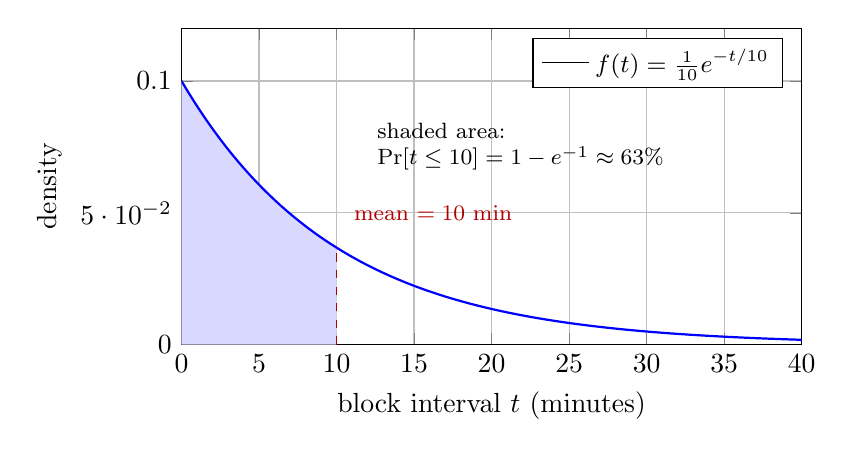
\begin{tikzpicture}
\begin{axis}[width=0.78\textwidth,height=5.6cm,xlabel={block interval $t$ (minutes)},ylabel={density},xmin=0,xmax=40,ymin=0,ymax=0.12,
 grid=both,ytick={0,0.05,0.1},legend style={font=\small,at={(0.97,0.97)},anchor=north east}]
\addplot[draw=none,fill=blue!15,domain=0:10,samples=60] {0.1*exp(-x/10)} \closedcycle;
\addplot[blue,thick,domain=0:40,samples=100] {0.1*exp(-x/10)};
\addlegendentry{$f(t)=\tfrac1{10}e^{-t/10}$}
\draw[dashed,red!70!black] (axis cs:10,0) -- (axis cs:10,0.0368);
\node[anchor=west,font=\footnotesize,red!70!black] at (axis cs:10.5,0.05) {mean $=10$ min};
\node[anchor=west,font=\footnotesize,align=left] at (axis cs:12,0.075) {shaded area:\\ $\Pr[t\le10]=1-e^{-1}\approx63\%$};
\end{axis}
\end{tikzpicture}
\caption{Block intervals are exponentially distributed (Theorem~\ref{thm:expo}). The median is $10\ln2\approx6.9$ minutes, and $\Pr[t>60\text{ min}]=e^{-6}\approx0.25\%$.}
\end{figure}

\subsection{Difficulty adjustment}

\begin{plainenglish}
If more miners join, blocks would come faster than every ten minutes. Bitcoin re-tunes the puzzle every 2016 blocks (about two weeks): if the last 2016 blocks arrived too fast, make the target smaller (harder);
if too slow, make it larger (easier). This thermostat keeps the \emph{rate} of blocks stable regardless of total hash power.
\end{plainenglish}

\begin{formal}
After every $2016$ blocks, with $\tau$ the actual time taken and $\tau_0=2016\times600\,\text{s}=14$ days,
$$T_{\text{new}}=T_{\text{old}}\cdot\frac{\operatorname{clamp}(\tau,\tau_0/4,4\tau_0)}{\tau_0}.$$
\end{formal}

\begin{exbox}[retarget]\label{ex:retarget}
The last 2016 blocks took $10$ days (hash rate went up). Then $T_{\text{new}}=T_{\text{old}}\cdot10/14\approx0.714\,T_{\text{old}}$: the target shrinks, puzzles are $1.4\times$ harder, and the expected block time returns to $10$ minutes.
If they had taken $70$ days, the clamp limits the change to $\times4$ (easier).
\end{exbox}

\begin{figure}[htbp]
\centering
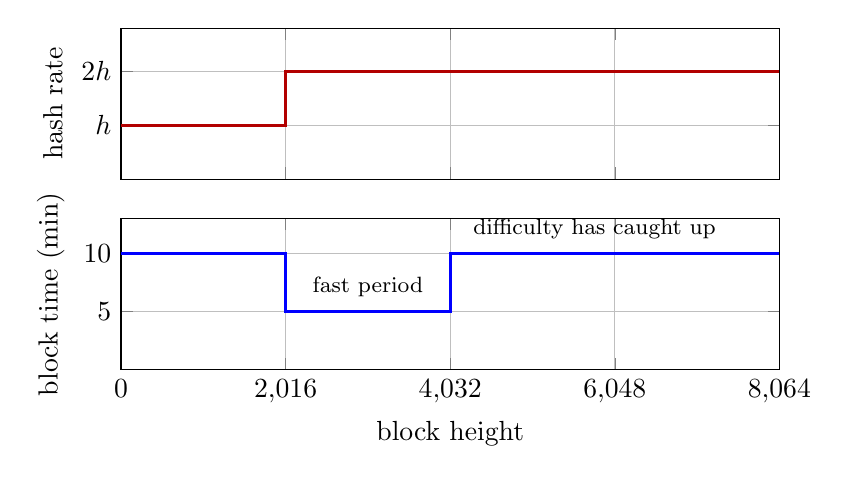
\begin{tikzpicture}
\begin{groupplot}[group style={group size=1 by 2,vertical sep=0.5cm,x descriptions at=edge bottom},
  width=0.82\textwidth,height=3.5cm,xmin=0,xmax=8064,xtick={0,2016,4032,6048,8064},grid=both,scaled x ticks=false]
\nextgroupplot[ylabel={hash rate},ymin=0,ymax=2.8,ytick={1,2},yticklabels={$h$,$2h$}]
\addplot[red!70!black,very thick,const plot] coordinates {(0,1) (2016,2) (8064,2)};
\nextgroupplot[ylabel={block time (min)},xlabel={block height},ymin=0,ymax=13,ytick={5,10}]
\addplot[blue,very thick] coordinates {(0,10) (2016,10) (2016,5) (4032,5) (4032,10) (8064,10)};
\node[font=\footnotesize,anchor=south] at (axis cs:3024,5.4) {fast period};
\node[font=\footnotesize,anchor=south] at (axis cs:5800,10.4) {difficulty has caught up};
\end{groupplot}
\end{tikzpicture}
\caption{Difficulty adjustment when the hash rate doubles right after a retarget. For one period blocks arrive every $5$ minutes; the next retarget halves the target (the period took $7$ days instead of $14$) and the interval returns to $10$ minutes.}
\end{figure}

\begin{remark}
Bitcoin's code measures the time between the first and the last block of a period, which spans only $2015$ intervals (a known off-by-one). The effect is $0.05\%$ and irrelevant for the analysis.
\end{remark}

\subsection{The longest-chain rule and forks}

\begin{plainenglish}
Two miners may find a block at nearly the same time. The network temporarily splits (a \emph{fork}). The rule is: ``always follow the valid chain with the most accumulated work, and keep mining on top of it''. Soon one branch gets the next
block and the other is abandoned (an \emph{orphan} or \emph{stale} block, its transactions return to the mempool). This is why a payment is considered safer the more blocks (\emph{confirmations}) are built on top of it.
\end{plainenglish}

\begin{figure}[htbp]
\centering
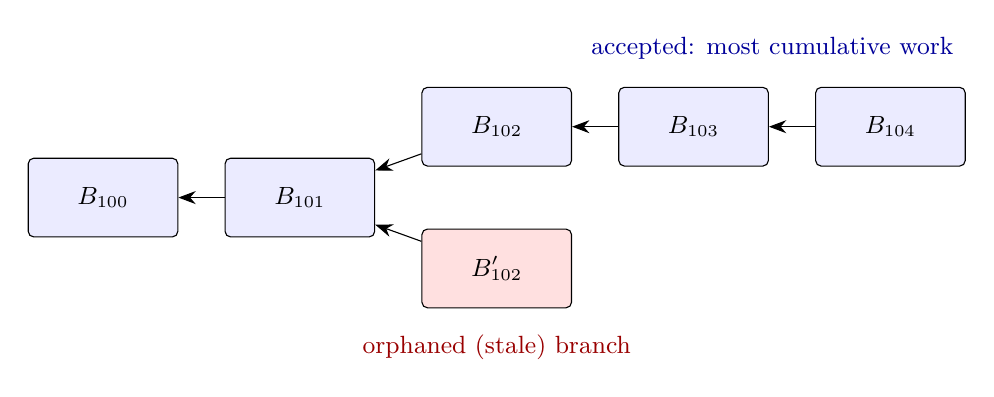
\begin{tikzpicture}
\node[blk] (g) at (0,0) {$B_{100}$};
\node[blk] (a) at (2.5,0) {$B_{101}$};
\node[blk] (b1) at (5,0.9) {$B_{102}$};
\node[blk,fill=red!12] (b2) at (5,-0.9) {$B'_{102}$};
\node[blk] (c) at (7.5,0.9) {$B_{103}$};
\node[blk] (d) at (10,0.9) {$B_{104}$};
\draw[->] (a)--(g); \draw[->] (b1)--(a); \draw[->] (b2)--(a); \draw[->] (c)--(b1); \draw[->] (d)--(c);
\node[font=\small,red!60!black] at (5,-1.9) {orphaned (stale) branch};
\node[font=\small,blue!60!black] at (8.5,1.9) {accepted: most cumulative work};
\end{tikzpicture}
\caption{A temporary fork resolved by the longest-chain (most-work) rule. Arrows point to the parent.}
\end{figure}

\begin{formal}
\begin{definition}[Chain work]
A chain $C=(B_1,\dots,B_\ell)$ whose blocks have targets $T_1,\dots,T_\ell$ has \emph{work} $W(C)=\sum_{i=1}^\ell \dfrac{2^{256}}{T_i+1}$, the expected number of hashes needed to produce it.
The rule: an honest node adopts the valid chain of maximum $W$ (ties broken by first-seen).
\end{definition}
\end{formal}

\begin{exercisebox}
\begin{enumerate}[nosep]
\item A transaction has input values $12.5$ and $3.2$ and outputs $10$, $5.6$ and $0.1$. Is it valid? What is the fee?
\item Why does using the number of blocks (rather than work) as the chain-selection rule become unsafe when difficulty can change?
\item Prove: $\Pr[\text{miner with fraction }\alpha\text{ finds }k\text{ of the next }m\text{ blocks}]=\binom mk\alpha^k(1-\alpha)^{m-k}$.
\item Suppose the 2016 blocks took 20 days. Compute $T_{\text{new}}/T_{\text{old}}$.
\item Estimate the number of leading zero bits needed if the network hash rate is $2\times10^{20}$ H/s.
\end{enumerate}
\end{exercisebox}
%================================================================
\section{Security Analysis of Nakamoto Consensus}\label{sec:security}
%================================================================

\subsection{The double-spend attack in plain terms}

\begin{plainenglish}
Mallory pays a merchant and waits for the payment to get buried under $z$ blocks. Meanwhile she secretly mines a competing chain in which the same coins go to herself. If her private chain ever becomes
longer than the public chain, she publishes it. Everyone switches (longest chain wins), the merchant's payment vanishes, but the goods have already been delivered. The question: \emph{how likely is
it that a private chain ever overtakes the public one?} The answer is the heart of Bitcoin's security: if Mallory has less than half the hash power, the probability shrinks \textbf{exponentially} in the number of confirmations $z$.
\end{plainenglish}

\begin{figure}[htbp]
\centering
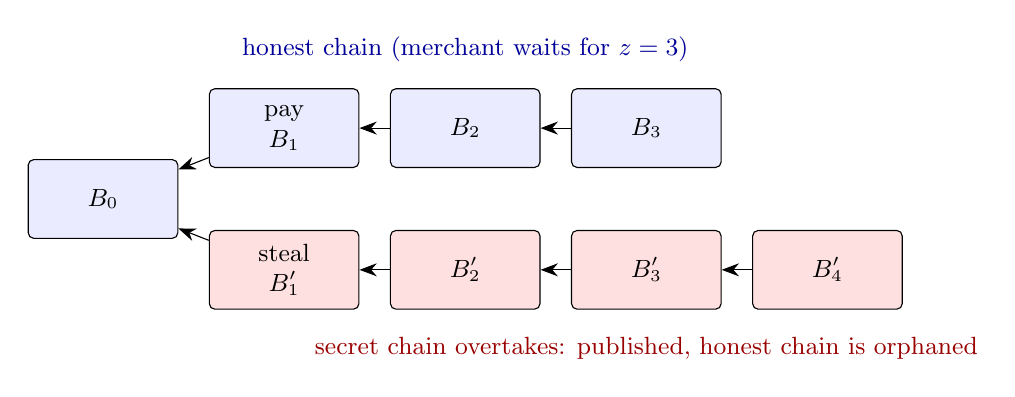
\begin{tikzpicture}
\node[blk] (g) at (0,0) {$B_0$};
\node[blk] (p1) at (2.3,0.9) {pay\\ $B_1$};
\node[blk] (p2) at (4.6,0.9) {$B_2$};
\node[blk] (p3) at (6.9,0.9) {$B_3$};
\node[adv] (a1) at (2.3,-0.9) {steal\\ $B'_1$};
\node[adv] (a2) at (4.6,-0.9) {$B'_2$};
\node[adv] (a3) at (6.9,-0.9) {$B'_3$};
\node[adv] (a4) at (9.2,-0.9) {$B'_4$};
\foreach \a/\b in {p1/g,p2/p1,p3/p2,a1/g,a2/a1,a3/a2,a4/a3}{\draw[->] (\a)--(\b);}
\node[font=\small,blue!60!black] at (4.6,1.9) {honest chain (merchant waits for $z=3$)};
\node[font=\small,red!60!black] at (6.9,-1.9) {secret chain overtakes: published, honest chain is orphaned};
\end{tikzpicture}
\caption{A double-spend: the attacker's secret chain (red) overtakes the honest chain.}
\end{figure}

\subsection{Gambler's ruin: the cleanest version}

\begin{formal}
Let $q$ be the attacker's share of hash power and $p=1-q$ the honest share. Each new block is found by the attacker with probability $q$ and by honest miners with probability $p$, independently
(Theorem~\ref{thm:expo} justifies this ``next block'' model). Let the attacker be $k$ blocks behind.

\begin{figure}[htbp]
\centering
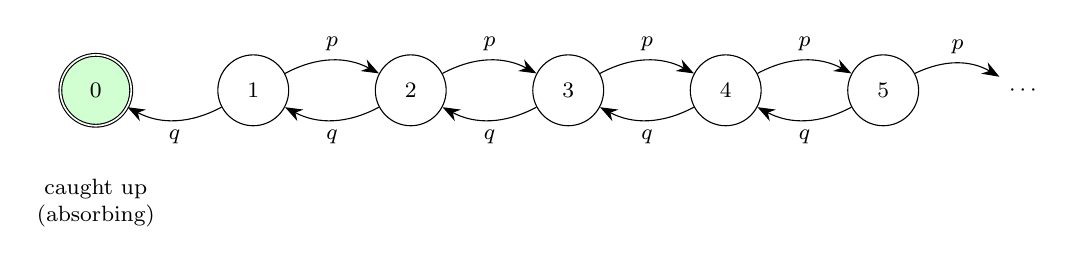
\begin{tikzpicture}[font=\footnotesize,
 s/.style={circle,draw,minimum size=0.9cm,fill=white,inner sep=0pt}]
\node[s,double,fill=green!18] (s0) at (0,0) {0};
\foreach \i in {1,...,5}{\node[s] (s\i) at (2*\i,0) {\i};}
\node (sd) at (11.8,0) {$\cdots$};
\foreach \i/\j in {1/0,2/1,3/2,4/3,5/4}{\draw[->] (s\i) to[bend left=28] node[below] {$q$} (s\j);}
\foreach \i/\j in {1/2,2/3,3/4,4/5}{\draw[->] (s\i) to[bend left=28] node[above] {$p$} (s\j);}
\draw[->] (s5) to[bend left=28] node[above] {$p$} (sd);
\node[below=0.55cm of s0,align=center] {caught up\\ (absorbing)};
\end{tikzpicture}
\caption{The attacker's deficit as a random walk. With probability $q$ she finds the next block (deficit $-1$), with probability $p=1-q$ the honest network does (deficit $+1$). Theorem~\ref{thm:gambler} gives the probability of ever reaching state $0$.}
\end{figure}

\begin{theorem}[Catch-up probability]\label{thm:gambler}
Let $f(k)$ be the probability that the attacker ever reaches a deficit of $0$ starting from deficit $k\ge0$. Then
$$f(k)=\begin{cases}(q/p)^k & q<p,\\ 1 & q\ge p.\end{cases}$$
\end{theorem}
\begin{proof}
Let $\rho=f(1)$. To go from deficit $k$ to $0$ the walk must successively reach $k-1,k-2,\dots,0$; by independence and time-homogeneity of the steps, $f(k)=\rho^k$.
Condition on the first step from deficit $1$: with probability $q$ the attacker finds a block and reaches $0$; with probability $p$ the deficit becomes $2$, from which the catch-up probability is $\rho^2$:
$$\rho=q+p\rho^2\iff p\rho^2-\rho+q=0\iff(\rho-1)(p\rho-q)=0.$$
So $\rho\in\{1,\,q/p\}$. Which root is it? Let $\rho_n$ be the probability of reaching $0$ from deficit $1$ within $n$ steps, so $\rho_0=0$ and $\rho_n\uparrow\rho$. Reaching $0$ from deficit $2$ within $n$ steps needs two successive catch-ups, which has probability at most $\rho_n^2$, so $\rho_{n+1}\le q+p\rho_n^2$. If $r\ge0$ is any root of the equation above, then $\rho_n\le r$ implies $\rho_{n+1}\le q+pr^2=r$; by induction $\rho_n\le r$ for all $n$, hence $\rho\le r$. Thus $\rho$ is a root that is at most every non-negative root, \ie\ the \emph{smallest} non-negative root. If $q<p$ then $q/p<1$ and $\rho=q/p$. If $q\ge p$ then $q/p\ge1$ and the smallest root is $1$. \qedhere
\end{proof}

\begin{corollary}[Exponential security]
For $q<1/2$, the probability that an attacker \emph{starting $z$ blocks behind} ever catches up is $(q/p)^z$, which decays exponentially in $z$. For $q\ge1/2$ the attacker eventually succeeds with probability~$1$ (the $51\%$ attack).
\end{corollary}
\begin{remark}
Conventions differ by one block: whether catching up to a \emph{tie} or strictly overtaking counts as success, and whether the block containing the payment is the first confirmation. This shifts $z$ by one and changes the numbers slightly, but never the exponential decay in $z$.
\end{remark}
\end{formal}

\begin{exbox}[the numbers]
$q=0.1$: $q/p=1/9$, so $z=6$ gives $(1/9)^6\approx1.9\times10^{-6}$. $q=0.3$: $q/p=3/7\approx0.4286$, so $z=6$ gives $\approx0.0062$, $z=10$ gives $0.0002$. For $q=0.45$: $q/p=0.818$ and $z=6$ gives $0.30$: a near-majority attacker is dangerous even after 6 confirmations.
\end{exbox}

\begin{figure}[htbp]
\centering
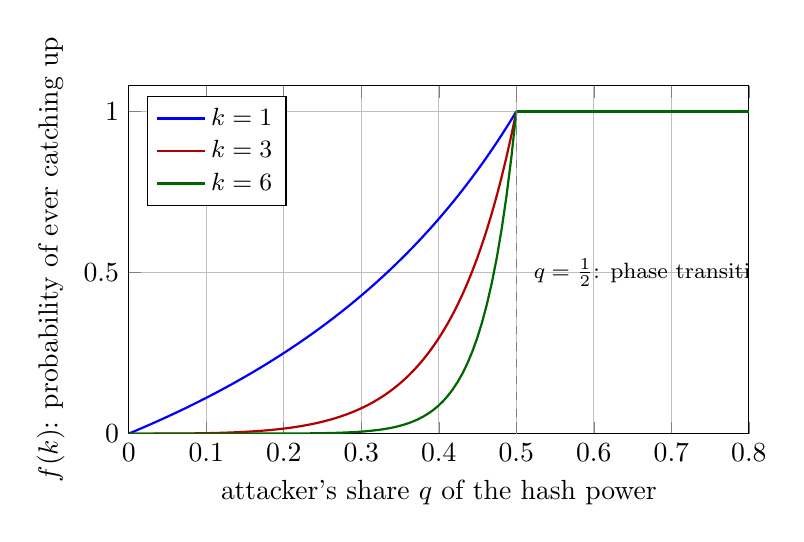
\begin{tikzpicture}
\begin{axis}[width=0.78\textwidth,height=6cm,xlabel={attacker's share $q$ of the hash power},ylabel={$f(k)$: probability of ever catching up},
 xmin=0,xmax=0.8,ymin=0,ymax=1.08,grid=both,legend pos=north west,legend style={font=\small}]
\addplot[blue,thick,domain=0:0.5,samples=80] {x/(1-x)};
\addplot[blue,thick,domain=0.5:0.8,forget plot] {1};
\addlegendentry{$k=1$}
\addplot[red!70!black,thick,domain=0:0.5,samples=80] {(x/(1-x))^3};
\addplot[red!70!black,thick,domain=0.5:0.8,forget plot] {1};
\addlegendentry{$k=3$}
\addplot[green!40!black,thick,domain=0:0.5,samples=80] {(x/(1-x))^6};
\addplot[green!40!black,thick,domain=0.5:0.8,forget plot] {1};
\addlegendentry{$k=6$}
\draw[dashed,gray] (axis cs:0.5,0) -- (axis cs:0.5,1.08);
\node[font=\footnotesize,anchor=west] at (axis cs:0.51,0.5) {$q=\tfrac12$: phase transition};
\end{axis}
\end{tikzpicture}
\caption{Catch-up probability $f(k)=\min\{1,(q/p)^k\}$ from Theorem~\ref{thm:gambler}. Below $q=1/2$ a deficit of $k=6$ is almost never recovered; at $q=1/2$ every deficit is eventually recovered.}
\end{figure}

\subsection{Nakamoto's calculation (accounting for the attacker's head start)}

\begin{plainenglish}
Theorem~\ref{thm:gambler} assumed the attacker is exactly $z$ behind. But while the honest network is busy finding those $z$ blocks, the attacker has also been mining in secret and has found some blocks of her own already.
Nakamoto's refinement averages over how many she has found.
\end{plainenglish}

\begin{formal}
While honest miners find $z$ blocks, the expected attacker progress is $\lambda=z\,q/p$. Nakamoto approximates the attacker's progress $K$ by a Poisson($\lambda$) variable. If $K=k\le z$ she is $z-k$ behind and later catches up with probability $(q/p)^{z-k}$; if $K>z$ she is already ahead. Hence
$$P_{\text{Nak}}(q,z)=1-\sum_{k=0}^{z}\frac{\lambda^ke^{-\lambda}}{k!}\Big(1-(q/p)^{z-k}\Big).$$
\begin{remark}[Exact version]
The number of attacker blocks before the $z$-th honest block is exactly negative binomial: $\Pr[K=k]=\binom{k+z-1}{k}p^zq^k$. Replacing the Poisson by this gives the exact probability
(Rosenfeld~\cite{Ros14}; Grunspan and P\'erez-Marco~\cite{GP18}) which is slightly larger, \eg\ about $0.0018$ instead of $0.0009$ for $q=0.1,z=5$. The qualitative conclusion is unchanged.
\end{remark}
\end{formal}

\begin{figure}[htbp]
\centering
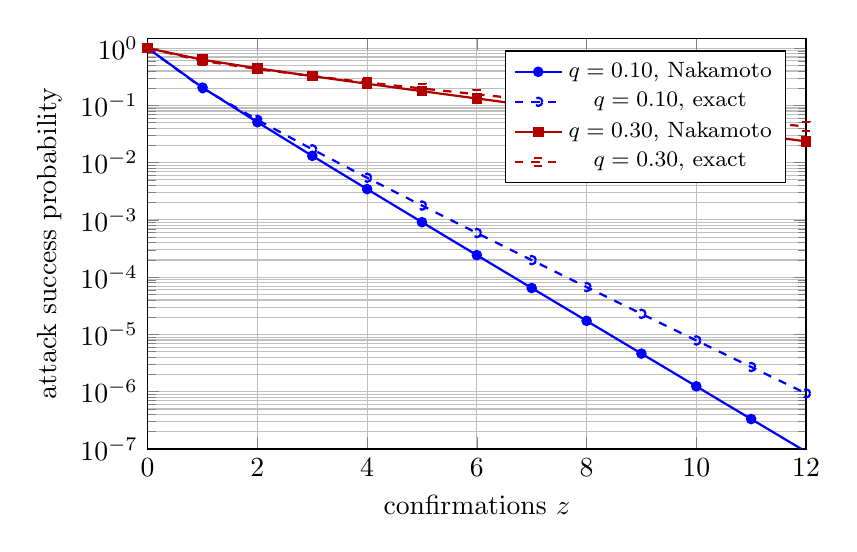
\begin{tikzpicture}
\begin{semilogyaxis}[width=0.82\textwidth,height=6.8cm,xlabel={confirmations $z$},ylabel={attack success probability},
  legend pos=north east,grid=both,ymin=1e-7,ymax=1.5,xmin=0,xmax=12,legend style={font=\footnotesize}]
\addplot[blue,thick,mark=*,mark size=1.5pt] coordinates {(0,1) (1,0.204587) (2,0.0509779) (3,0.0131722) (4,0.00345524) (5,0.000913682) (6,0.000242803) (7,6.47353e-05) (8,1.72998e-05) (9,4.63116e-06) (10,1.2414e-06) (11,3.33108e-07) (12,8.94584e-08)};
\addlegendentry{$q=0.10$, Nakamoto}
\addplot[blue,thick,dashed,mark=o,mark size=1.5pt] coordinates {(0,1) (1,0.2) (2,0.056) (3,0.01712) (4,0.005456) (5,0.00178184) (6,0.000591412) (7,0.000198571) (8,6.72498e-05) (9,2.29289e-05) (10,7.85976e-06) (11,2.70613e-06) (12,9.35154e-07)};
\addlegendentry{$q=0.10$, exact}
\addplot[red!70!black,thick,mark=square*,mark size=1.5pt] coordinates {(0,1) (1,0.627749) (2,0.445717) (3,0.324584) (4,0.239127) (5,0.177352) (6,0.132111) (7,0.0987125) (8,0.0739244) (9,0.0554572) (10,0.0416605) (11,0.0313309) (12,0.023584)};
\addlegendentry{$q=0.30$, Nakamoto}
\addplot[red!70!black,thick,dashed,mark=square,mark size=1.5pt] coordinates {(0,1) (1,0.6) (2,0.432) (3,0.32616) (4,0.252072) (5,0.197617) (6,0.15645) (7,0.12475) (8,0.100025) (9,0.0805539) (10,0.0651067) (11,0.0527799) (12,0.042896)};
\addlegendentry{$q=0.30$, exact}
\end{semilogyaxis}
\end{tikzpicture}
\caption{Double-spend success probability: Nakamoto's Poisson approximation (solid) versus the exact negative-binomial value (dashed). Straight lines on a log scale mean exponential decay; the Poisson approximation \emph{underestimates} the risk, increasingly so for large $z$.}
\end{figure}

\begin{exbox}[confirmations needed]\label{ex:confirm}
Number of confirmations so that the success probability is below $0.1\%$. With Nakamoto's approximation: $z=5$ for $q=0.1$ ($P=0.0009137$) and $z=24$ for $q=0.3$. With the exact formula the answers are larger, $z=6$ and $z=32$ (Figure~\ref{fig:zneeded}). This is the origin of the folklore ``wait for 6 confirmations'', tuned for attackers with $q\approx10\%$.
Because blocks arrive every $10$ minutes, $6$ confirmations take about an hour.
\end{exbox}

\begin{center}
\small
\begin{tabular}{@{}rcccc@{}}
\toprule
 & \multicolumn{2}{c}{$q=0.1$} & \multicolumn{2}{c}{$q=0.3$}\\
$z$ & Nakamoto & Exact & Nakamoto & Exact\\
\midrule
1 & 0.2046 & 0.2000 & 0.6277 & 0.6000\\
2 & 0.0510 & 0.0560 & 0.4457 & 0.4320\\
3 & 0.0132 & 0.0171 & 0.3246 & 0.3262\\
5 & 0.0009 & 0.0018 & 0.1774 & 0.1976\\
10 & $1.2\cdot10^{-6}$ & $7.9\cdot10^{-6}$ & 0.0417 & 0.0651\\
\bottomrule
\end{tabular}
\end{center}
(Exact values computed numerically from the negative-binomial formula.)

\begin{figure}[htbp]
\centering
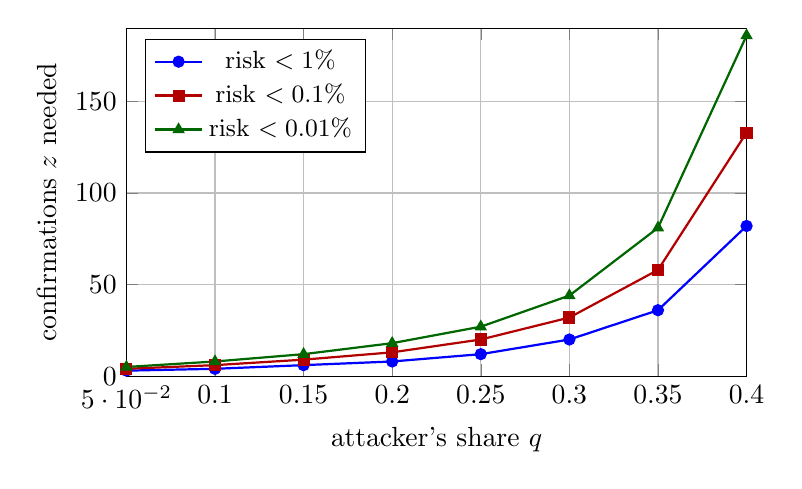
\begin{tikzpicture}
\begin{axis}[width=0.78\textwidth,height=6cm,xlabel={attacker's share $q$},ylabel={confirmations $z$ needed},
 xmin=0.05,xmax=0.40,ymin=0,ymax=190,grid=both,legend pos=north west,legend style={font=\small},mark size=1.8pt]
\addplot[blue,thick,mark=*] coordinates {(0.05,3) (0.1,4) (0.15,6) (0.2,8) (0.25,12) (0.3,20) (0.35,36) (0.4,82)};
\addlegendentry{risk $<1\%$}
\addplot[red!70!black,thick,mark=square*] coordinates {(0.05,4) (0.1,6) (0.15,9) (0.2,13) (0.25,20) (0.3,32) (0.35,58) (0.4,133)};
\addlegendentry{risk $<0.1\%$}
\addplot[green!40!black,thick,mark=triangle*] coordinates {(0.05,5) (0.1,8) (0.15,12) (0.2,18) (0.25,27) (0.3,44) (0.35,81) (0.4,186)};
\addlegendentry{risk $<0.01\%$}
\end{axis}
\end{tikzpicture}
\caption{Confirmations needed so that the exact double-spend probability is below a given risk. The ``six confirmations'' rule is right for attackers with $q\lesssim10\%$ and a $0.1\%$ risk; it explodes as $q\to1/2$.}
\label{fig:zneeded}
\end{figure}

\subsection{Beyond one attack: the Bitcoin Backbone model}

\begin{plainenglish}
The double-spend calculation analyses \emph{one specific attack}. A cryptographer wants to prove that \emph{no attack} works. The Bitcoin Backbone framework (Garay, Kiayias, Leonardos 2015) does that by isolating three clean
properties of the chain that hold with overwhelming probability when honest miners hold a majority, and then derives the ledger guarantees (persistence and liveness) from them:
\begin{itemize}[nosep]
\item \textbf{Common prefix}: honest nodes' chains agree except for the last few blocks.
\item \textbf{Chain growth}: the chain keeps growing at a guaranteed minimum speed.
\item \textbf{Chain quality}: a guaranteed fraction of any long stretch of the chain was mined by honest miners (so the adversary cannot censor everything).
\end{itemize}
\end{plainenglish}

\begin{formal}
Let $\mathcal C_1,\mathcal C_2$ denote chains held by honest parties, and $\mathcal C^{\lceil k}$ the chain with its last $k$ blocks removed.
\begin{definition}[Backbone properties]
\begin{itemize}[nosep]
\item \emph{Common prefix} (parameter $k$): for any two honest chains $\mathcal C_1,\mathcal C_2$ at rounds $r_1\le r_2$, $\mathcal C_1^{\lceil k}\preceq\mathcal C_2$ (prefix relation).
\item \emph{Chain growth} $(\tau,s)$: for any honest chain at rounds $r_1<r_2$ with $r_2-r_1\ge s$, the chain has grown by at least $\tau(r_2-r_1)$ blocks.
\item \emph{Chain quality} $(\mu,\ell)$: in any $\ell$ consecutive blocks of an honest chain, at least a $\mu$ fraction were mined by honest parties.
\end{itemize}
\end{definition}

\begin{figure}[htbp]
\centering
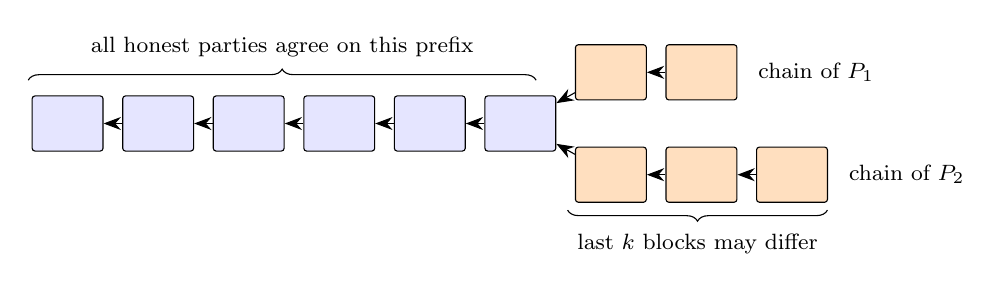
\begin{tikzpicture}[font=\footnotesize,
 b/.style={draw,rounded corners=1pt,minimum width=0.9cm,minimum height=0.7cm,fill=blue!10},
 u/.style={b,fill=orange!25}]
\foreach \i in {0,...,5}{\node[b] (c\i) at (1.15*\i,0) {};}
\foreach \i/\j in {1/0,2/1,3/2,4/3,5/4}{\draw[->] (c\i)--(c\j);}
\node[u] (p1) at (6.9,0.65) {}; \node[u] (p2) at (8.05,0.65) {};
\node[u] (q1) at (6.9,-0.65) {}; \node[u] (q2) at (8.05,-0.65) {}; \node[u] (q3) at (9.2,-0.65) {};
\draw[->] (p1)--(c5); \draw[->] (p2)--(p1); \draw[->] (q1)--(c5); \draw[->] (q2)--(q1); \draw[->] (q3)--(q2);
\node[anchor=west] at (8.65,0.65) {chain of $P_1$}; \node[anchor=west] at (9.8,-0.65) {chain of $P_2$};
\draw[decorate,decoration={brace,amplitude=4pt}] (-0.5,0.55) -- (5.95,0.55) node[midway,above=5pt] {all honest parties agree on this prefix};
\draw[decorate,decoration={brace,amplitude=4pt,mirror}] (6.35,-1.1) -- (9.65,-1.1) node[midway,below=5pt] {last $k$ blocks may differ};
\end{tikzpicture}
\caption{Common prefix (parameter $k$): after removing the last $k$ blocks, the chain of one honest party is a prefix of the other's. The finalized ledger $\mathsf L$ of Definition~\ref{def:ledger} is exactly this stable prefix.}
\end{figure}

\begin{theorem}[Backbone, informal \cite{GKL15,PSS17}]\label{thm:backbone}
In the synchronous model with network delay $\Delta$, let $\alpha$ be the probability that at least one honest party finds a block in a round and $\beta$ the expected number of blocks the adversary finds in a round.
If the honest-majority condition $\alpha\big(1-2(\Delta+1)\alpha\big)>(1+\delta)\beta$ holds for some constant $\delta>0$, then common prefix, chain growth and chain quality hold except with probability $e^{-\Omega(k)}$.
Consequently persistence holds with parameter $k$, and liveness with $u=O(k)$.
\end{theorem}

We prove the simplest piece, \emph{chain growth}, and sketch common prefix.
\begin{lemma}[Chain growth, $\Delta=0$]
In every round an honest party finds a block with probability $\alpha$. Then in any $s$ rounds, the honest chain grows by at least $(1-\epsilon)\alpha s$ blocks except with probability $\le e^{-\epsilon^2\alpha s/2}$.
\end{lemma}
\begin{proof}
With zero delay, every round in which some honest party succeeds extends the longest honest chain by at least one block. Let $X_j\in\{0,1\}$ indicate success in round $j$. Then $X=\sum_{j=1}^sX_j$ is binomial with mean $\alpha s$,
and the multiplicative Chernoff bound gives $\Pr[X\le(1-\epsilon)\alpha s]\le e^{-\epsilon^2\alpha s/2}$.
\end{proof}

\emph{Sketch of common prefix.} Call a round a \emph{convergence opportunity} if exactly one honest party finds a block in it and none do in the surrounding $\Delta$ rounds. Such a block is unique at its height and all honest parties adopt it. Two honest chains that disagree
on a block $k$ deep force the adversary to build a competing branch: every convergence opportunity adds an honest block to the common branch, while a competing branch can only grow through adversarial blocks. Over a window of $m$ rounds, the number of convergence opportunities is about $\alpha(1-2(\Delta+1)\alpha)m$,
and the number of adversarial blocks is about $\beta m$. If the former exceeds the latter (honest-majority condition), Chernoff bounds show that the adversary cannot keep a fork of depth $k$ alive except with probability $e^{-\Omega(k)}$.
\end{formal}

\subsection{Selfish mining}

\begin{plainenglish}
Is it \emph{rational} for miners to follow the protocol? Eyal and Sirer (2014) showed that a pool with only a fraction of the hash power can earn \emph{more than its fair share} of rewards by hiding the blocks it finds, and releasing them
strategically to waste the honest miners' work. Honest miners keep working on the old tip, while the selfish miners are ahead on a private chain. When the honest miners catch up, the selfish pool reveals its chain just in time to orphan their blocks.
The attack works even though the pool has less than $50\%$ of the hash power, which is the threshold Nakamoto's analysis suggested was safe.
\end{plainenglish}

\begin{figure}[htbp]
\centering
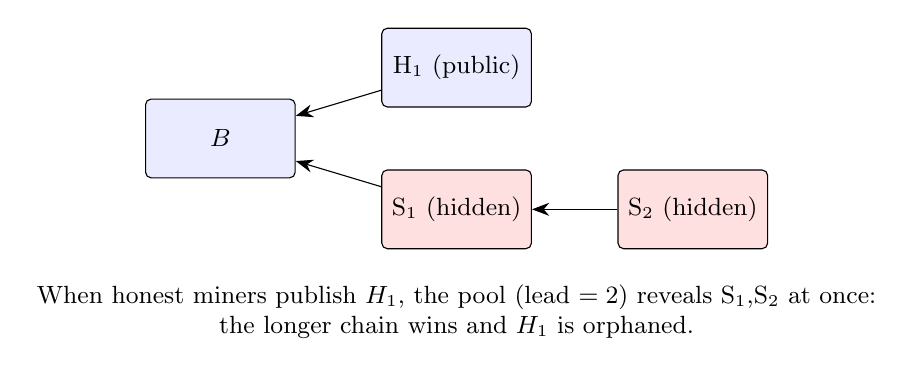
\begin{tikzpicture}
\node[blk] (g) at (0,0) {$B$};
\node[blk] (h1) at (3,0.9) {H$_1$ (public)};
\node[adv] (s1) at (3,-0.9) {S$_1$ (hidden)};
\node[adv] (s2) at (6,-0.9) {S$_2$ (hidden)};
\draw[->] (h1)--(g); \draw[->] (s1)--(g); \draw[->] (s2)--(s1);
\node[font=\small,align=center] at (3,-2.2) {When honest miners publish $H_1$, the pool (lead $=2$) reveals S$_1$,S$_2$ at once:\\ the longer chain wins and $H_1$ is orphaned.};
\end{tikzpicture}
\caption{Selfish mining with a lead of $2$. The pool publishes its private chain when the honest network is about to catch up.}
\end{figure}

\begin{formal}
\begin{theorem}[Eyal--Sirer \cite{ES14}]
Let the selfish pool have fraction $\alpha$ and let $\gamma\in[0,1]$ be the fraction of honest hash power that mines on the pool's block during a tie. Following the selfish strategy, the pool's relative revenue is
$$R_{\text{pool}}=\frac{\alpha(1-\alpha)^2\big(4\alpha+\gamma(1-2\alpha)\big)-\alpha^3}{1-\alpha\big(1+(2-\alpha)\alpha\big)},$$
and selfish mining is strictly more profitable than honest mining ($R_{\text{pool}}>\alpha$) exactly when $\alpha>\dfrac{1-\gamma}{3-2\gamma}$.
\end{theorem}
The formula comes from the stationary distribution of a Markov chain whose state is the length of the pool's private lead (states $0,0',1,2,\dots$). We omit that derivation and instead check the claimed threshold.
\end{formal}

\begin{figure}[htbp]
\centering
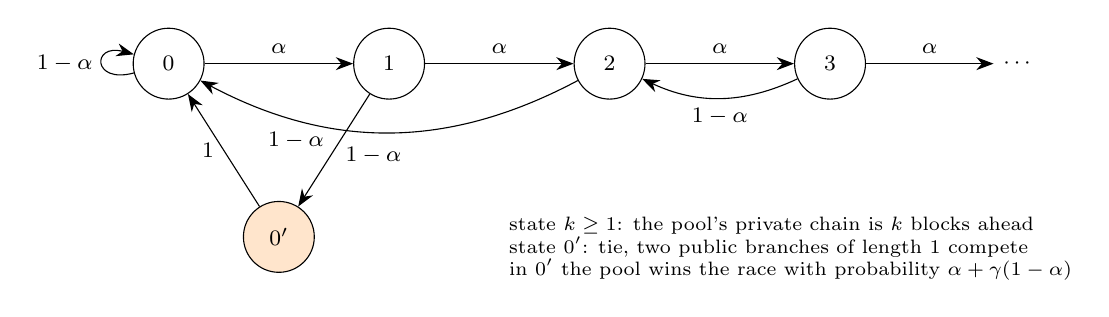
\begin{tikzpicture}[font=\footnotesize,
 s/.style={circle,draw,minimum size=0.9cm,fill=white,inner sep=0pt}]
\node[s] (s0) at (0,0) {0};
\node[s] (s1) at (2.8,0) {1};
\node[s] (s2) at (5.6,0) {2};
\node[s] (s3) at (8.4,0) {3};
\node (sd) at (10.8,0) {$\cdots$};
\node[s,fill=orange!20] (s0p) at (1.4,-2.2) {$0'$};
\draw[->] (s0) to[loop left,looseness=6] node[left] {$1-\alpha$} (s0);
\draw[->] (s0) -- node[above] {$\alpha$} (s1);
\draw[->] (s1) -- node[above] {$\alpha$} (s2);
\draw[->] (s2) -- node[above] {$\alpha$} (s3);
\draw[->] (s3) -- node[above] {$\alpha$} (sd);
\draw[->] (s1) -- node[right,pos=0.55,xshift=2pt] {$1-\alpha$} (s0p);
\draw[->] (s0p) -- node[left,pos=0.5] {$1$} (s0);
\draw[->] (s2) to[bend left=28] node[below,pos=0.75,yshift=-1pt] {$1-\alpha$} (s0);
\draw[->] (s3) to[bend left=25] node[below] {$1-\alpha$} (s2);
\node[align=left,anchor=west,font=\scriptsize] at (4.2,-2.35) {state $k\ge1$: the pool's private chain is $k$ blocks ahead\\ state $0'$: tie, two public branches of length $1$ compete\\ in $0'$ the pool wins the race with probability $\alpha+\gamma(1-\alpha)$};
\end{tikzpicture}
\caption{The Markov chain behind the Eyal--Sirer revenue formula. A pool block (probability $\alpha$) lengthens the private lead; an honest block (probability $1-\alpha$) shortens it. At lead $2$ the pool publishes everything and returns to state $0$.}
\end{figure}

\begin{exbox}[threshold check at $\gamma=0$]\label{ex:selfish}
At $\gamma=0$ the threshold is $\alpha=1/3$. Plug $\alpha=1/3$ into the formula: numerator $=\tfrac13\cdot\tfrac49\cdot\tfrac43-\tfrac1{27}=\tfrac{16}{81}-\tfrac{3}{81}=\tfrac{13}{81}$; denominator $=1-\tfrac13\big(1+\tfrac53\cdot\tfrac13\big)=1-\tfrac{14}{27}=\tfrac{13}{27}$.
So $R_{\text{pool}}=\tfrac{13/81}{13/27}=\tfrac13=\alpha$: exactly break-even, as claimed. Other thresholds: $\gamma=\tfrac12\Rightarrow\alpha>\tfrac14$; $\gamma=1\Rightarrow\alpha>0$ (any pool profits).
\end{exbox}

\begin{figure}[htbp]
\centering
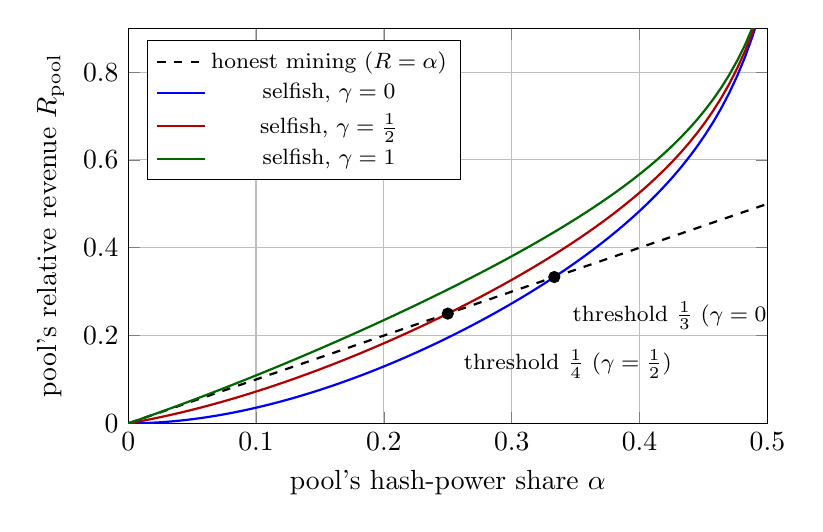
\begin{tikzpicture}
\begin{axis}[width=0.8\textwidth,height=6.6cm,xlabel={pool's hash-power share $\alpha$},ylabel={pool's relative revenue $R_{\text{pool}}$},
 xmin=0,xmax=0.5,ymin=0,ymax=0.9,grid=both,legend pos=north west,legend style={font=\footnotesize}]
\addplot[black,dashed,thick,domain=0:0.5] {x};
\addlegendentry{honest mining ($R=\alpha$)}
\addplot[blue,thick,domain=0:0.495,samples=80] {(x*(1-x)^2*(4*x+0*(1-2*x))-x^3)/(1-x*(1+(2-x)*x))};
\addlegendentry{selfish, $\gamma=0$}
\addplot[red!70!black,thick,domain=0:0.495,samples=80] {(x*(1-x)^2*(4*x+0.5*(1-2*x))-x^3)/(1-x*(1+(2-x)*x))};
\addlegendentry{selfish, $\gamma=\tfrac12$}
\addplot[green!40!black,thick,domain=0:0.495,samples=80] {(x*(1-x)^2*(4*x+1*(1-2*x))-x^3)/(1-x*(1+(2-x)*x))};
\addlegendentry{selfish, $\gamma=1$}
\addplot[only marks,mark=*,mark size=2pt,black] coordinates {(0.3333,0.3333) (0.25,0.25)};
\node[font=\footnotesize,anchor=north west] at (axis cs:0.34,0.30) {threshold $\tfrac13$ ($\gamma=0$)};
\node[font=\footnotesize,anchor=north west] at (axis cs:0.255,0.19) {threshold $\tfrac14$ ($\gamma=\tfrac12$)};
\end{axis}
\end{tikzpicture}
\caption{Revenue of a selfish pool (Eyal--Sirer formula) against honest mining. Where a coloured curve rises above the dashed line, selfish mining pays; the crossing points are the thresholds $\alpha=\frac{1-\gamma}{3-2\gamma}$.}
\end{figure}

\noindent\textbf{Caveats.} ``Revenue'' is the pool's share of the blocks that end up in the main chain. Selfish mining orphans honest blocks, so the \emph{rate} of main-chain blocks drops, and the attack pays in absolute terms only after the next difficulty adjustment. A countermeasure proposed by Eyal and Sirer, choosing uniformly at random among equally long branches, raises the threshold to $\alpha=1/4$.

\subsection{51\% attacks and what they can and cannot do}

\begin{plainenglish}
An attacker with a majority of the hash power can rewrite recent history (double-spend), and can censor transactions. She \emph{cannot} forge signatures (so cannot steal coins she does not own), cannot create coins beyond the
block reward, and cannot change the consensus rules that honest full nodes enforce. Smaller chains have suffered real $51\%$ attacks (Ethereum Classic, Bitcoin Gold) because hash power for small coins can be rented cheaply.
\end{plainenglish}

\begin{exercisebox}
\begin{enumerate}[nosep]
\item Verify Theorem~\ref{thm:gambler} numerically: for $q=0.4$, $k=3$ compute $(q/p)^3$. Simulate (by hand or code) the random walk to confirm.
\item Compute $P_{\text{Nak}}(0.25,4)$ with $\lambda=4\cdot\tfrac13$. 
\item Show that for $q<1/2$ the Nakamoto sum can also be written as $\sum_{k=0}^{z}\Pr[K=k](q/p)^{z-k}+\Pr[K>z]$.
\item Use the formula in Example~\ref{ex:selfish} to compute $R_{\text{pool}}$ for $\alpha=0.4,\gamma=0.5$. Is selfish mining profitable?
\item Why does a larger network delay $\Delta$ favour the adversary in Theorem~\ref{thm:backbone}?
\end{enumerate}
\end{exercisebox}
%================================================================
\section{Consensus Theory}\label{sec:consensus}
%================================================================

\subsection{The Byzantine agreement problem}

\begin{plainenglish}
Imagine several generals surrounding a city. They must \emph{all} attack or \emph{all} retreat, communicating only by messengers, and some generals are traitors who may tell different generals different things.
Can the loyal generals reach the same decision? This is \textbf{Byzantine agreement}, the theoretical ancestor of blockchain consensus. The surprising answer: it depends sharply on the assumptions (timing, number of traitors,
signatures), and for some settings it is \emph{impossible}.
\end{plainenglish}

\begin{formal}
\begin{definition}[Byzantine agreement (consensus)]
$n$ parties, each with an input bit; up to $f$ are Byzantine. A protocol solves consensus if for every execution:
\begin{itemize}[nosep]
\item \textbf{Agreement}: all honest parties output the same value;
\item \textbf{Validity}: if all honest parties have the same input $v$, they output $v$;
\item \textbf{Termination}: all honest parties eventually output.
\end{itemize}
\end{definition}

\begin{theorem}[Lamport--Shostak--Pease~\cite{LSP82}; Pease--Shostak--Lamport~\cite{PSL80}]\label{thm:3f}
Without digital signatures (``oral messages''), consensus is solvable for $n$ parties among which $f$ are Byzantine if and only if $n\ge 3f+1$.
\end{theorem}
\begin{proof}[Proof of impossibility for $n=3$, $f=1$ (the hexagon argument)]
Suppose a protocol exists for $A,B,C$ with one traitor. Build a hexagon of six machines $A_0,B_0,C_0,A_1,B_1,C_1$ running the three roles in a ring, where $A_0,B_0,C_0$ have input $0$ and $A_1,B_1,C_1$ have input $1$.
\begin{center}
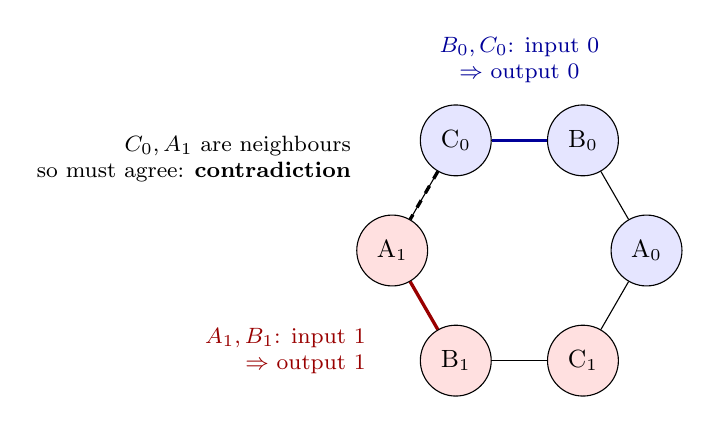
\begin{tikzpicture}[scale=0.95,font=\footnotesize]
\foreach \i/\n/\col in {0/A$_0$/blue!10,1/B$_0$/blue!10,2/C$_0$/blue!10,3/A$_1$/red!12,4/B$_1$/red!12,5/C$_1$/red!12}{
  \node[node,fill=\col] (h\i) at ({60*\i}:1.7) {\n};
}
\foreach \i/\j in {0/1,1/2,2/3,3/4,4/5,5/0}{\draw (h\i)--(h\j);}
\draw[very thick,blue!60!black] (h1)--(h2);
\draw[very thick,red!60!black] (h3)--(h4);
\draw[very thick,dashed] (h2)--(h3);
\node[align=center,blue!60!black] at (90:2.55) {$B_0,C_0$: input $0$\\ $\Rightarrow$ output $0$};
\node[align=right,red!60!black,anchor=east] at (215:2.35) {$A_1,B_1$: input $1$\\ $\Rightarrow$ output $1$};
\node[align=right,anchor=east] at (150:2.45) {$C_0,A_1$ are neighbours\\ so must agree: \textbf{contradiction}};
\end{tikzpicture}
\end{center}
Consider the adjacent machines $B_0,C_0$. Each sees one neighbour playing ``$A$'' (for $B_0$ it is $A_0$, for $C_0$ it is $A_1$) and the other honest neighbour. This is exactly what honest $B$ and $C$ see in the real three-party system when the traitor $A$ behaves like $A_0$ towards $B$ and like $A_1$ towards $C$. Both have input $0$, so validity forces $B_0$ and $C_0$ to output $0$. The same argument applied to $A_1,B_1$ (both input $1$, with a traitor $C$ imitating $C_0$ towards $A_1$ and $C_1$ towards $B_1$) shows that they output $1$. Now look at the adjacent pair $C_0,A_1$: their views are those of honest $C$ and $A$ in a real run in which $B$ is the traitor, behaving like $B_0$ towards $C$ and like $B_1$ towards $A$. Agreement demands equal outputs, but $C_0$ outputs $0$ and $A_1$ outputs $1$. Contradiction.
\end{proof}
\begin{remark}
For general $n\le3f$, split the parties into three groups of at most $f$ and let each group simulate one of the three generals; a protocol for $n\le 3f$ would then give one for $n=3$, $f=1$, which does not exist.
\end{remark}
\end{formal}

\begin{exbox}[why 3 is not enough]
Three generals $A,B,C$ with $C$ a traitor. $A$ says ``attack'' to $B$. $C$ tells $B$ ``$A$ told me retreat''. $B$ sees ``attack'' from $A$ and ``retreat'' from $C$ and cannot tell whether $A$ or $C$ is lying. With $4$ generals and one traitor, the
loyal ones take a \emph{majority} of the other three reports and the traitor is outvoted.
\end{exbox}

\subsection{Timing: synchrony, partial synchrony, asynchrony}

\begin{plainenglish}
How long can a message take? If we know a hard upper bound (synchrony), a missing message means a crashed or lying peer. If delays are unbounded (asynchrony), we cannot tell a slow peer from a dead peer. The famous \textbf{FLP result}
shows that in a fully asynchronous system even \emph{one crash} makes deterministic consensus impossible. Real protocols escape it by either assuming partial synchrony (PBFT), using randomness (Ben-Or, HoneyBadger),
or using a lottery plus time (Nakamoto).
\end{plainenglish}

\begin{formal}
\begin{theorem}[Fischer--Lynch--Paterson~\cite{FLP85}]
No deterministic protocol in the asynchronous model solves consensus (with termination) if even one party may crash.
\end{theorem}
\emph{Proof sketch.} Call a configuration \emph{bivalent} if both decisions $0$ and $1$ are still reachable, and \emph{univalent} otherwise. (1) There is a bivalent initial configuration: change the inputs one party at a time from all-$0$ (decides $0$) to all-$1$ (decides $1$);
some adjacent pair of input vectors differing in party $p$ gives different decisions; crash $p$ and the other parties cannot tell the two apart, so the configuration is bivalent. (2) From any bivalent configuration the adversarial scheduler can deliver messages so that the next configuration is again bivalent:
for a pending message $m$, consider the set of configurations reachable without delivering $m$ and then delivering $m$; a case analysis on commuting events shows one of them is bivalent. Hence an infinite execution without decision exists. $\square$

\begin{definition}[Partial synchrony, Dwork--Lynch--Stockmeyer~\cite{DLS88}]
There is an unknown global stabilisation time (GST) after which all messages arrive within a bound $\Delta$. Safety must hold always; liveness is only required after GST.
\end{definition}
\begin{theorem}[DLS 1988]
Partially synchronous Byzantine consensus is solvable iff $n\ge3f+1$.
\end{theorem}
\end{formal}

\subsection{PBFT: practical Byzantine fault tolerance}

\begin{plainenglish}
PBFT (Castro--Liskov~\cite{CL99}) has a rotating \emph{leader} (primary). The leader proposes a value; replicas then exchange two rounds of votes (``prepare'' and ``commit''). A replica decides when it has seen \emph{more than two thirds}
of the replicas agree twice. Why two rounds of voting? The first makes sure everyone agrees about what the leader proposed (even a lying leader cannot show different things to different replicas), the second makes sure that enough replicas know that this agreement happened, so that if a new leader takes over,
the decision is not lost.
\end{plainenglish}

\begin{figure}[htbp]
\centering
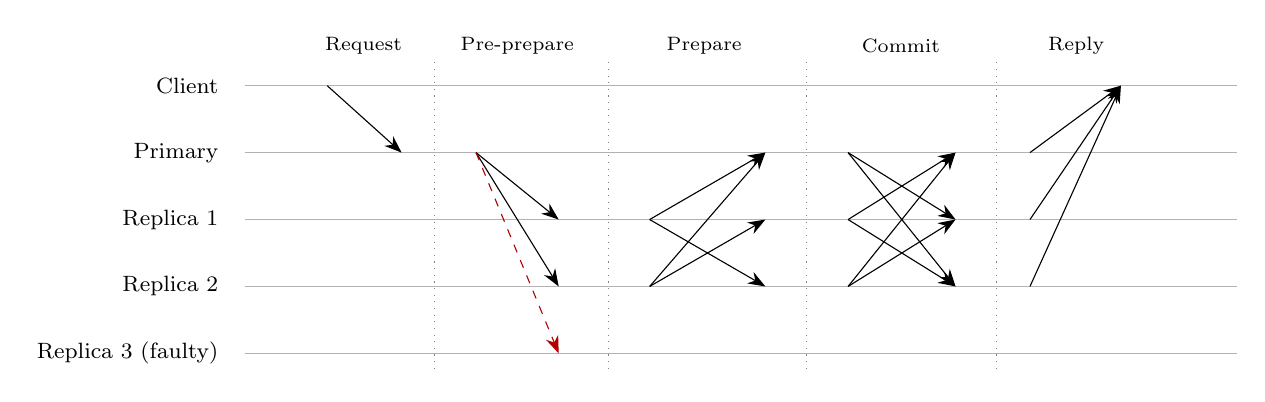
\begin{tikzpicture}[xscale=2.1,yscale=0.85,font=\footnotesize]
\foreach \i/\n in {0/Client,1/Primary,2/Replica 1,3/Replica 2,4/Replica 3 (faulty)}{
  \node[left] at (-0.1,-\i) {\n};
  \draw[gray!60] (0,-\i)--(6,-\i);
}
\foreach \x/\l in {0.72/Request,1.65/Pre-prepare,2.78/Prepare,3.97/Commit,5.03/Reply}{\node[font=\scriptsize] at (\x,0.6) {\l};}
\foreach \x in {1.15,2.2,3.4,4.55}{\draw[dotted,gray] (\x,0.35)--(\x,-4.3);}
\draw[->] (0.5,0)--(0.95,-1);
\draw[->] (1.4,-1)--(1.9,-2); \draw[->] (1.4,-1)--(1.9,-3); \draw[->,dashed,red!70!black] (1.4,-1)--(1.9,-4);
\foreach \a in {2,3}{\foreach \b in {1,2,3}{\ifnum\a=\b\else\draw[->,thin] (2.45,-\a)--(3.15,-\b);\fi}}
\foreach \a in {1,2,3}{\foreach \b in {1,2,3}{\ifnum\a=\b\else\draw[->,thin] (3.65,-\a)--(4.3,-\b);\fi}}
\foreach \a in {1,2,3}{\draw[->] (4.75,-\a)--(5.3,0);}
\end{tikzpicture}
\caption{PBFT message flow with $n=4$ and $f=1$; replica~3 is faulty and silent. The primary's pre-prepare plays the role of its prepare, so only backups send prepare messages; all replicas send commits. The client accepts after $f+1$ matching replies. Communication is $O(n^2)$ per decision.}
\end{figure}

\begin{formal}
\begin{theorem}[Quorum intersection]\label{thm:quorum}
Let $n=3f+1$ and let a quorum be any set of $2f+1$ parties. Then any two quorums intersect in at least $f+1$ parties, hence in at least one honest party.
\end{theorem}
\begin{proof}
$|Q_1\cap Q_2|\ge|Q_1|+|Q_2|-n=2(2f+1)-(3f+1)=f+1$. At most $f$ of these are Byzantine, so at least one is honest.
\end{proof}

\begin{figure}[htbp]
\centering
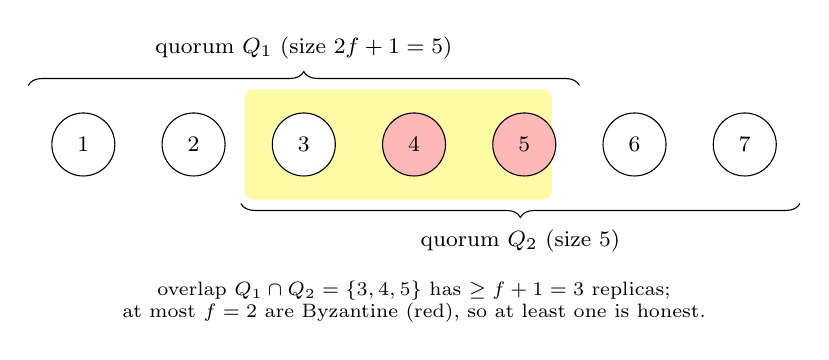
\begin{tikzpicture}[font=\footnotesize,
 p/.style={circle,draw,minimum size=0.8cm,fill=white}]
\begin{scope}[on background layer]
\fill[yellow!35,rounded corners=3pt] (3.45,-0.7) rectangle (7.35,0.7);
\end{scope}
\foreach \i in {1,2,3,6,7}{\node[p] (n\i) at (1.4*\i,0) {\i};}
\foreach \i in {4,5}{\node[p,fill=red!28] (n\i) at (1.4*\i,0) {\i};}
\draw[decorate,decoration={brace,amplitude=5pt}] (0.7,0.75) -- (7.7,0.75) node[midway,above=6pt] {quorum $Q_1$ (size $2f+1=5$)};
\draw[decorate,decoration={brace,amplitude=5pt,mirror}] (3.4,-0.75) -- (10.5,-0.75) node[midway,below=6pt] {quorum $Q_2$ (size $5$)};
\node[font=\scriptsize,align=center] at (5.6,-2.0) {overlap $Q_1\cap Q_2=\{3,4,5\}$ has $\ge f+1=3$ replicas;\\ at most $f=2$ are Byzantine (red), so at least one is honest.};
\end{tikzpicture}
\caption{Quorum intersection for $n=7$, $f=2$. Any two quorums overlap in an honest replica, which cannot vote for two conflicting values.}
\end{figure}

In PBFT with $n=3f+1$ a replica is \emph{prepared} once it holds the pre-prepare and $2f$ matching prepares from distinct backups, and it \emph{commits locally} once it is prepared and has $2f+1$ matching commits (its own included). Both certificates are quorums of size $2f+1$.

\begin{corollary}[PBFT safety]
Suppose two honest replicas commit different values $v\ne v'$ in the same view and sequence number. Each needed a commit quorum $Q$, $Q'$ of $2f+1$ replicas that sent matching prepare/commit messages. By Theorem~\ref{thm:quorum} some honest replica is in both quorums, but an honest replica sends
only one prepare message per (view, sequence), a contradiction. Safety thus holds with up to $f$ Byzantine replicas \emph{regardless of timing}; liveness needs partial synchrony (view-change timeouts).
\end{corollary}
\end{formal}

\begin{exbox}[numbers for $n=4$, $n=7$, $n=100$]
\begin{center}\small
\begin{tabular}{@{}cccc@{}}
\toprule
$n$ & max faulty $f=\lfloor(n-1)/3\rfloor$ & quorum $2f+1$ & overlap of two quorums\\
\midrule
4 & 1 & 3 & $\ge2$\\
7 & 2 & 5 & $\ge3$\\
100 & 33 & 67 & $\ge34$\\
\bottomrule
\end{tabular}
\end{center}
With $n=4$, a leader and 3 replicas: messages per decision: $3$ (pre-prepare) $+\,3\cdot3$ (prepare) $+\,4\cdot3$ (commit) $=24$; in general $(n-1)+(n-1)^2+n(n-1)=2n(n-1)$. With $n=100$ it is $19{,}800\approx2\cdot10^4$ messages: this is why classical BFT does not scale to thousands of anonymous miners.
\end{exbox}

\subsection{Nakamoto consensus versus classical BFT}

\begin{center}
\small
\begin{tabular}{@{}p{3.1cm}p{5.4cm}p{5.4cm}@{}}
\toprule
 & \textbf{Nakamoto (PoW)} & \textbf{Classical BFT (PBFT)}\\
\midrule
Participants & open, anonymous & known, fixed committee\\
Sybil defence & computational work & membership list\\
Fault tolerance & $<50\%$ of hash power & $<33\%$ of parties\\
Timing assumption & synchronous (bounded $\Delta$ relative to block time) & partial synchrony\\
Finality & probabilistic (confirmations) & deterministic, immediate\\
Scalability in $n$ & excellent (no all-to-all) & poor ($O(n^2)$ messages)\\
\bottomrule
\end{tabular}
\end{center}

\begin{plainenglish}
Why can PoW tolerate $50\%$ but BFT only $33\%$? In PBFT, a quorum must work even if $f$ parties are silent and $f$ are lying; this costs a third. In PoW, the \emph{synchrony assumption} is stronger: honest blocks eventually reach everyone and the adversary has only a bounded ability to delay.
Under pure asynchrony, no protocol can tolerate a majority; the price Bitcoin pays is the assumption that block time is long compared with network delay. The tolerable fraction also shrinks as the delay $\Delta$ grows relative to the block time (Theorem~\ref{thm:backbone}); $50\%$ is the limit only for an instantaneous network.
\end{plainenglish}

\subsection{Proof of Stake}

\begin{plainenglish}
Proof of Work wastes energy as the Sybil defence. \textbf{Proof of Stake} replaces ``hash power'' with ``coins locked up as collateral''. The next block proposer is chosen by a stake-weighted lottery (a validator with $10\%$ of the staked coins is chosen about $10\%$ of the time), and misbehaviour is punished by
\emph{slashing} (destroying) the stake. New problems appear because creating blocks is free:
\begin{itemize}[nosep]
\item \textbf{Nothing-at-stake}: on a fork, a validator can vote for \emph{both} branches at no cost. Fix: slashing for double-voting.
\item \textbf{Long-range attack}: an attacker who bought (or bribed) old keys can rewrite history from far in the past, cheaply. Fix: \emph{weak subjectivity} (new nodes must obtain a recent checkpoint from a trusted source) and key-evolving signatures.
\item \textbf{Grinding}: the attacker tries many ways to bias the randomness of the lottery. Fix: secure randomness beacons (VRFs, commit-reveal).
\end{itemize}
\end{plainenglish}

\begin{formal}
\textbf{Ouroboros-style leader election~\cite{KRDO17}.} Time is divided into slots. For slot $t$ and validator $i$ with relative stake $\sigma_i$, validator $i$ is eligible if $\mathsf{VRF}_{\sk_i}(\eta\concat t)<\phi(\sigma_i)=1-(1-f_{\text{act}})^{\sigma_i}$, where $\eta$ is epoch randomness and $f_{\text{act}}$ is the fraction of slots with a leader. The function $\phi$ is chosen so that a stakeholder's chance
does not change if it splits its stake among many identities (``sybil-neutrality''): $1-\prod_j(1-\phi(\sigma_j))=1-(1-f_{\text{act}})^{\sum\sigma_j}$.

\textbf{Accountable safety (Casper FFG~\cite{BG17}).} Validators vote on checkpoint pairs (source$\to$target). Two slashing conditions: (1) no two different votes with the same target height; (2) no vote whose span strictly surrounds another of the same validator's votes. A vote is a \emph{supermajority link} if validators with $\ge2/3$ of the stake cast it. A checkpoint is \emph{justified} if it is the target of a supermajority link from a justified checkpoint, and \emph{finalized} if it is justified and a supermajority link leads from it to its direct child checkpoint.

\begin{figure}[htbp]
\centering
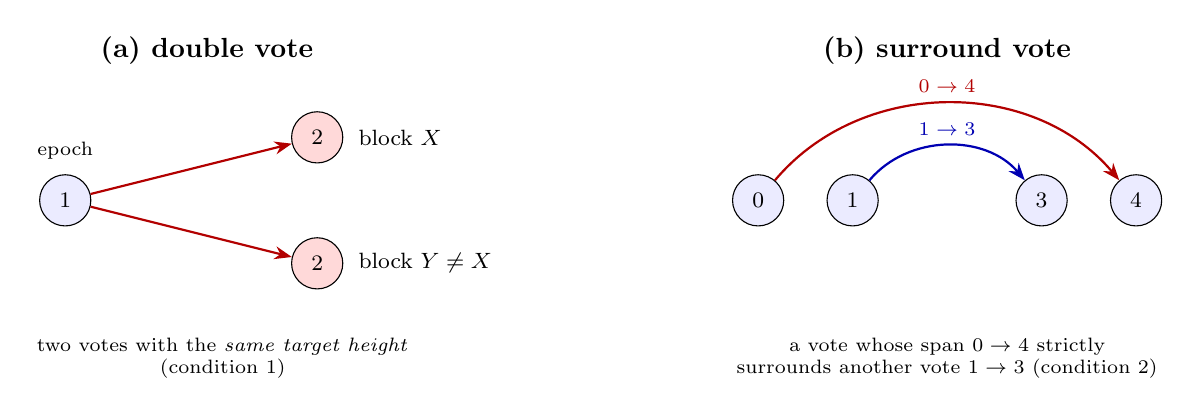
\begin{tikzpicture}[font=\footnotesize,
 cp/.style={circle,draw,minimum size=0.65cm,inner sep=0pt,fill=blue!8}]
\node[font=\bfseries] at (1.8,1.9) {(a) double vote};
\node[cp] (s) at (0,0) {1}; \node[cp,fill=red!15] (a) at (3.2,0.8) {2}; \node[cp,fill=red!15] (b) at (3.2,-0.8) {2};
\draw[->,thick,red!70!black] (s)--(a); \draw[->,thick,red!70!black] (s)--(b);
\node[right=2pt of a] {block $X$}; \node[right=2pt of b] {block $Y\neq X$}; \node[above=2pt of s,font=\scriptsize] {epoch};
\node[align=center,font=\scriptsize] at (2.0,-2.0) {two votes with the \emph{same target height}\\ (condition 1)};
\begin{scope}[xshift=8.8cm]
\node[font=\bfseries] at (2.4,1.9) {(b) surround vote};
\foreach \e/\x in {0/0,1/1.2,3/3.6,4/4.8}{\node[cp] (e\e) at (\x,0) {\e};}
\draw[->,thick,red!70!black,bend left=50] (e0) to node[above,font=\scriptsize,pos=0.5] {$0\to4$} (e4);
\draw[->,thick,blue!70!black,bend left=50] (e1) to node[above,font=\scriptsize,pos=0.5] {$1\to3$} (e3);
\node[align=center,font=\scriptsize] at (2.4,-2.0) {a vote whose span $0\to4$ strictly\\ surrounds another vote $1\to3$ (condition 2)};
\end{scope}
\end{tikzpicture}
\caption{The two Casper FFG slashing conditions. Both can be proved from the two signed votes alone.}
\end{figure}
\begin{theorem}[Accountable safety]
If two conflicting checkpoints are both finalized, then at least $1/3$ of the total stake can be proven to have violated a slashing condition.
\end{theorem}
\begin{proof}[Proof idea]
Each finalized checkpoint is backed by a set of validators with at least $2/3$ of the stake. Two such sets overlap in at least $2/3+2/3-1=1/3$ of the stake (this is Theorem~\ref{thm:quorum} in fractional form). A validator in the overlap voted for two conflicting checkpoints,
and a case analysis on heights shows that it must have violated condition (1) or (2). The cryptographic signatures on the votes are the evidence. Hence safety violations are not only unlikely but \emph{economically expensive}: the adversary loses at least one third of the stake.
\end{proof}
\end{formal}

\begin{exbox}[cost of attacking a PoS chain]
If the total stake is $30$ million coins worth $\$2000$ each ($\$60$B), breaking finality costs the attacker at least a third of it (slashed): $\$20$B. An equal-hash-power PoW attack is not slashed: the attacker's ASICs remain after the attack.
This ``loss of capital on attack'' is the main security selling point of PoS, together with energy savings.
\end{exbox}

\begin{exercisebox}
\begin{enumerate}[nosep]
\item For $n=10$, what is the maximum $f$? What is the quorum size? How many honest replicas are guaranteed in the intersection of any two quorums?
\item Show that if quorums have size $\lceil(n+f+1)/2\rceil$, any two intersect in $\ge f+1$ parties. For $n=3f+1$ what size is that?
\item Why does the hexagon argument break if digital signatures are available (with a PKI)? What is the new bound for signed messages (Dolev--Strong)?
\item Explain why a ``nothing-at-stake'' validator earns strictly more by voting on both branches if there is no slashing.
\item Check sybil-neutrality: show $(1-f_{\text{act}})^{\sigma_1}(1-f_{\text{act}})^{\sigma_2}=(1-f_{\text{act}})^{\sigma_1+\sigma_2}$.
\end{enumerate}
\end{exercisebox}
%================================================================
\section{Smart Contracts and Ethereum}\label{sec:eth}
%================================================================

\subsection{From transactions to programs}

\begin{plainenglish}
Bitcoin's ledger answers ``who owns which coins?''. Ethereum~\cite{Woo14} generalises it to a \emph{shared computer}: the ledger stores not only balances but also \textbf{programs} (smart contracts) and their memory.
Anyone can send a transaction that calls a program; every node runs it and must reach the same result. Think of a vending machine that nobody owns: you put coins in and the code, not a person, decides what happens.
Ethereum uses \textbf{accounts} (like a bank: each address has a balance and a counter) rather than UTXOs. Since September 2022 (``The Merge'') Ethereum uses proof of stake: block producers are \emph{validators} rather than miners, but the transaction and state model described here is unchanged.
\end{plainenglish}

\begin{center}\small
\begin{tabular}{@{}p{3cm}p{5.6cm}p{5.6cm}@{}}
\toprule
 & \textbf{UTXO (Bitcoin)} & \textbf{Account (Ethereum)}\\
\midrule
State & set of unspent outputs & map address $\to$ (balance, nonce, code, storage)\\
Replay protection & each output spent once & per-account nonce\\
Parallelism & easy (independent outputs) & harder (shared state)\\
Programmability & limited Script & Turing-complete EVM\\
Privacy & better (fresh addresses per payment) & worse (one address, visible history)\\
\bottomrule
\end{tabular}
\end{center}

\begin{figure}[htbp]
\centering
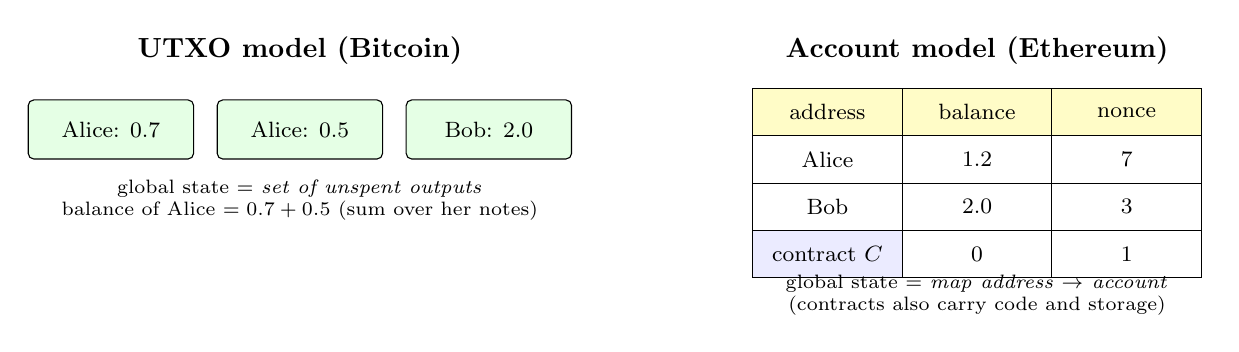
\begin{tikzpicture}[font=\footnotesize,
 nt/.style={draw,rounded corners=2pt,fill=green!10,minimum width=2.1cm,minimum height=0.75cm,align=center}]
\node[font=\bfseries] at (2.4,2.1) {UTXO model (Bitcoin)};
\node[nt] at (0,1.1) {Alice: $0.7$}; \node[nt] at (2.4,1.1) {Alice: $0.5$}; \node[nt] at (4.8,1.1) {Bob: $2.0$};
\node[align=center,font=\scriptsize] at (2.4,0.2) {global state = \emph{set of unspent outputs}\\ balance of Alice $=0.7+0.5$ (sum over her notes)};
\node[font=\bfseries] at (11,2.1) {Account model (Ethereum)};
\matrix[matrix of nodes,nodes={draw,minimum width=1.9cm,minimum height=0.6cm,font=\footnotesize,anchor=center},
  row sep=-\pgflinewidth,column sep=-\pgflinewidth,anchor=north] at (11,1.75) {
 |[fill=yellow!22]| address & |[fill=yellow!22]| balance & |[fill=yellow!22]| nonce\\
 Alice & $1.2$ & $7$\\
 Bob & $2.0$ & $3$\\
 |[fill=blue!8]| contract $C$ & $0$ & $1$\\
};
\node[align=center,font=\scriptsize] at (11,-1.0) {global state = \emph{map address $\to$ account}\\ (contracts also carry code and storage)};
\end{tikzpicture}
\caption{The same economic situation in the two ledger models. A UTXO payment consumes and creates notes; an account payment decreases one balance, increases another and increments the sender's nonce.}
\end{figure}

\begin{formal}
\begin{definition}[Ethereum as a state machine]
Global state $\sigma$ maps each address to a tuple $(\mathsf{nonce},\allowbreak\mathsf{balance},\allowbreak\mathsf{codeHash},\allowbreak\mathsf{storageRoot})$. A transaction $T$ induces the deterministic transition $\sigma'=\Upsilon(\sigma,T)$; a block applies its transactions in order. The state is committed in the block header
by the root of a \emph{Merkle--Patricia trie} (a Merkle tree over a radix trie keyed by address), so a light client can verify any account's balance with a logarithmic proof, exactly as in Theorem~\ref{thm:merkle}.
\end{definition}
\end{formal}

\subsection{Gas: taming the halting problem}

\begin{plainenglish}
If contracts can loop forever, one malicious transaction could freeze every node. Ethereum charges for every step: each EVM instruction costs \emph{gas}, the sender pre-pays a gas limit, and execution is aborted when the gas runs out (all effects are
rolled back, but the fee is lost). So a program with an infinite loop simply runs out of money.
\end{plainenglish}

\begin{formal}
Since EIP-1559~\cite{EIP1559}, each block has a gas target $G^*$ and a limit $2G^*$. The \emph{base fee} adjusts as
$$b_{t+1}=b_t\left(1+\frac{1}{8}\cdot\frac{g_t-G^*}{G^*}\right),$$
where $g_t$ is the gas used in block $t$. The base fee is burned; the tip goes to the block proposer. A full block ($g_t=2G^*$) raises $b$ by $12.5\%$; an empty block lowers it by $12.5\%$.
\end{formal}

\begin{exbox}[fee dynamics]
Let $b_t=20$ gwei, target $15$M gas. Block $t$ uses $30$M (full): $b_{t+1}=20\cdot1.125=22.5$ gwei. If the next block is empty: $b_{t+2}=22.5\cdot0.875\approx19.7$ gwei. A simple transfer uses $21{,}000$ gas, so at $22.5$ gwei the base fee is $21000\cdot22.5\cdot10^{-9}=0.0004725$ ETH.
\end{exbox}

\subsection{Writing contracts and what goes wrong: reentrancy}

\begin{plainenglish}
Smart contracts hold real money and cannot be patched once deployed, so bugs are expensive. The most famous bug class is \textbf{reentrancy}: a contract sends money to an address \emph{before} updating its own books. If the receiver is itself a contract, its code runs
when it receives the money and can call back into the first contract while its books still say ``you still have a balance''. The attacker withdraws repeatedly. This is how ``The DAO'' lost about 3.6 million ETH in 2016, leading to the Ethereum/Ethereum Classic split.
\end{plainenglish}

\begin{lstlisting}[language=Solidity,caption={A vulnerable bank contract}]
contract Bank {
    mapping(address => uint) public balance;
    function deposit() public payable { balance[msg.sender] += msg.value; }
    function withdraw() public {
        uint amount = balance[msg.sender];
        (bool ok, ) = msg.sender.call{value: amount}("");  // (1) interaction first
        require(ok);
        balance[msg.sender] = 0;                           // (2) effect too late!
    }
}
\end{lstlisting}

\begin{figure}[htbp]
\centering
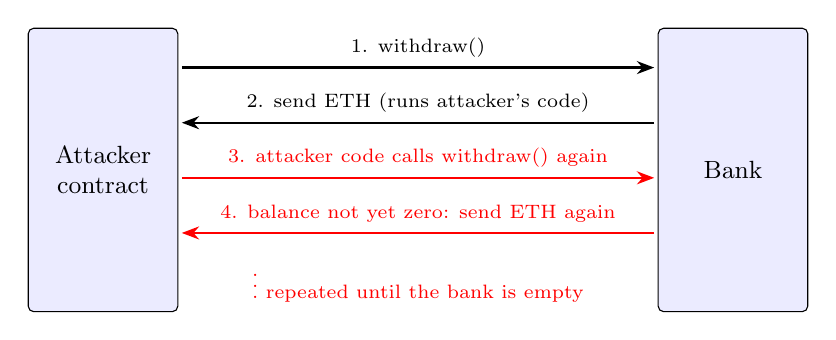
\begin{tikzpicture}
\node[blk,minimum height=3.6cm] (att) at (0,0) {Attacker\\ contract};
\node[blk,minimum height=3.6cm] (bank) at (8,0) {Bank};
\draw[->,thick] (1,1.3) -- node[above,font=\scriptsize]{1. withdraw()} (7,1.3);
\draw[->,thick] (7,0.6) -- node[above,font=\scriptsize]{2. send ETH (runs attacker's code)} (1,0.6);
\draw[->,thick,red] (1,-0.1) -- node[above,font=\scriptsize,red]{3. attacker code calls withdraw() again} (7,-0.1);
\draw[->,thick,red] (7,-0.8) -- node[above,font=\scriptsize,red]{4. balance not yet zero: send ETH again} (1,-0.8);
\node[font=\scriptsize,red] at (4,-1.4) {$\vdots$ repeated until the bank is empty};
\end{tikzpicture}
\caption{Reentrancy: the bank pays before it zeroes the balance.}
\end{figure}

\begin{exbox}[draining a bank]
The bank holds $100$ ETH from others. The attacker deposits $1$ ETH and calls \texttt{withdraw}. The bank sends $1$ ETH, the attacker's fallback calls \texttt{withdraw} again; \texttt{balance[attacker]} is still $1$, so the bank sends another $1$ ETH, and so on.
After $101$ nested calls the bank is empty, and only then does each call return and set \texttt{balance=0}. The attacker turned $1$ ETH into $101$ ETH.
\end{exbox}

\textbf{The fix} is the \emph{checks-effects-interactions} pattern: update the state (set \texttt{balance=0}) \emph{before} sending money, or use a reentrancy lock.

\begin{formal}
\textbf{Why formal methods?} A contract $C$ with state space $S$ and transition relation $\to$ should satisfy an invariant $I$: $I(s_0)$ and $\forall s\to s'.\ I(s)\Rightarrow I(s')$. For the bank, $I$ is ``$\sum_a\mathsf{balance}[a]\le$ contract ETH''.
Reentrancy breaks $I$ at an intermediate state when an external call hands control to untrusted code. Verification tools (model checking, SMT-based tools, the K framework, Certora) check such invariants or prove their absence of violation.
The unusual feature is the stakes: the code is public, immutable and holds money.
\end{formal}

\begin{exercisebox}
\begin{enumerate}[nosep]
\item Rewrite the \texttt{withdraw} function using checks-effects-interactions.
\item Compute the base fee after three consecutive full blocks starting at $10$ gwei.
\item State an invariant for a token contract with \texttt{totalSupply} and \texttt{balanceOf}, and explain which operations could violate it.
\item Why must contract execution be deterministic? Name three EVM-visible sources of non-determinism that are therefore forbidden or controlled.
\end{enumerate}
\end{exercisebox}

%================================================================
\section{Privacy-Preserving Blockchains}\label{sec:privacy}
%================================================================

\begin{plainenglish}
Bitcoin is \emph{pseudonymous}, not anonymous: every transaction is public forever and addresses can be linked (clustering) and tied to real identities when coins touch an exchange. Privacy coins try to hide the \textbf{sender}, the \textbf{receiver} and the \textbf{amount}, while still letting everyone verify
that no coins were created from nothing. The tools: \emph{commitments} (hide a number but fix it), \emph{ring signatures} (``one of these ten people signed''), and \emph{zero-knowledge proofs} (``I know a valid secret, but I won't tell you which one'').
\end{plainenglish}

\subsection{Pedersen commitments and confidential amounts}

\begin{plainenglish}
A commitment is a sealed envelope: you put a number inside, seal it, and hand it over. Later you can open it, but you cannot change the number in the meantime (\emph{binding}), and nobody can see inside before you open it (\emph{hiding}).
Pedersen commitments have a special trick: if you add two sealed envelopes, you get a sealed envelope containing the \emph{sum}. So a network can check that ``inputs equal outputs'' without ever seeing the amounts.
\end{plainenglish}

\begin{formal}
Let $\G$ have prime order $q$, with generators $g,h$ such that $\log_gh$ is unknown to everyone.
\begin{definition}[Pedersen commitment~\cite{Ped91}]
$\mathsf{Com}(m;r)=g^mh^r$, with $m,r\in\Z_q$.
\end{definition}
\begin{theorem}\label{thm:pedersen}
(i) \emph{Perfectly hiding}: for any $m$, $\mathsf{Com}(m;r)$ with $r\leftarrow_\$\Z_q$ is uniform in $\G$. (ii) \emph{Computationally binding} under discrete log. (iii) \emph{Homomorphic}: $\mathsf{Com}(m_1;r_1)\cdot\mathsf{Com}(m_2;r_2)=\mathsf{Com}(m_1+m_2;r_1+r_2)$.
\end{theorem}
\begin{proof}
(i) $h$ generates $\G$, so $r\mapsto h^r$ is a bijection and $g^mh^r$ is uniform. (ii) If $\Adv$ opens one commitment to $(m,r)\ne(m',r')$ with $m\neq m'$ (if $m=m'$ then $r=r'$), then $g^mh^r=g^{m'}h^{r'}$, so $g^{m-m'}=h^{r'-r}$ and $r'\neq r$; thus
$\log_gh=(m-m')(r'-r)^{-1}\bmod q$, solving discrete log. (iii) $g^{m_1}h^{r_1}g^{m_2}h^{r_2}=g^{m_1+m_2}h^{r_1+r_2}$.
\end{proof}
\end{formal}

\begin{exbox}[Pedersen with numbers]\label{ex:pedersen}
In the group of order $q=11$ inside $\Z_{23}^*$: $g=4$, $h=9$. Commit to $m_1=3$ with $r_1=2$: $C_1=4^3\cdot9^2=64\cdot81\equiv18\cdot12=216\equiv9$. Commit to $m_2=4$ with $r_2=5$: $C_2=4^4\cdot9^5\equiv3\cdot8=24\equiv1$.
Product: $C_1C_2=9$. And $\mathsf{Com}(7;7)=4^7\cdot9^7=36^7\equiv13^7\equiv9$ \checkmark. The sum of the hidden values ($3+4=7$) is verified without revealing $3$ or $4$. (In this toy group $h=g^8$ is known, so the commitment is not binding; in practice $h$ is derived by hashing, so that nobody knows $\log_gh$.)
\end{exbox}

\textbf{Confidential transactions.} Each output amount $v_j$ is replaced by $C_j=g^{v_j}h^{r_j}$. A validator checks that $\prod_{\text{in}}C_i\big/\big(g^{\text{fee}}\prod_{\text{out}}C_j\big)$ is a commitment to $0$, \ie\ equals $h^{\Delta r}$ for a known $\Delta r$ (shown by a signature under the public key $h^{\Delta r}$ with base $h$).

\begin{warnbox}[(why range proofs are needed)]
Working modulo $q$, an output of $-5$ is just $q-5$. A cheater can create outputs $(+10)$ and $(-5)$ from an input of $5$: the sum matches, yet the attacker has minted $5$ coins. Hence each hidden amount must come with a zero-knowledge \textbf{range proof} that $0\le v<2^{64}$
(Bulletproofs~\cite{BMRS16} make these logarithmic in size).
\end{warnbox}

\subsection{Ring signatures (Monero)}

\begin{plainenglish}
To hide \emph{who} is paying, Monero lets the sender sign with a \textbf{ring signature}: ``this transaction was authorised by one of these 16 public keys'', where 15 are decoys taken from the blockchain. A verifier is convinced that a ring member signed but
cannot tell which. To prevent the same coin being spent twice from different rings, each real key produces a unique \textbf{key image} $I=x\cdot\Hash_p(P)$; two spends with the same key image are rejected, yet the key image does not reveal which ring member it belongs to.
\end{plainenglish}

\begin{exbox}[ring size and anonymity]\label{ex:ring}
With ring size $16$ and an observer who knows nothing else, each member is the signer with probability $1/16=6.25\%$. If $10$ of the decoys are known to be already spent elsewhere (so cannot be the signer), the anonymity set shrinks to $6$ and the probability rises to $1/6\approx16.7\%$.
Privacy degrades when external information (timing, spent-output analysis) is available.
\end{exbox}

\begin{figure}[htbp]
\centering
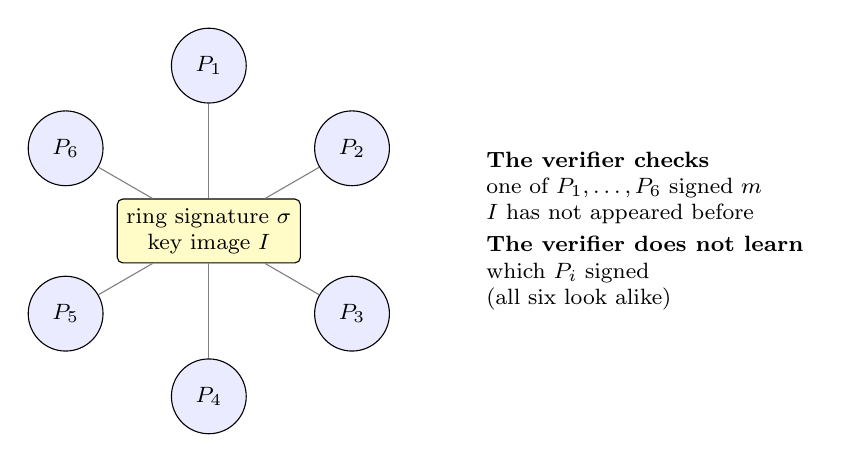
\begin{tikzpicture}[font=\footnotesize,
 k/.style={circle,draw,minimum size=0.95cm,fill=blue!8}]
\foreach \i in {1,...,6}{\node[k] (p\i) at ({90-60*(\i-1)}:2.1) {$P_{\i}$};}
\node[draw,rounded corners=2pt,fill=yellow!22,align=center] (sg) at (0,0) {ring signature $\sigma$\\ key image $I$};
\foreach \i in {1,...,6}{\draw[gray] (p\i)--(sg);}
\node[align=left,anchor=west] at (3.4,0) {\textbf{The verifier checks}\\ one of $P_1,\ldots,P_6$ signed $m$\\ $I$ has not appeared before\\[2pt] \textbf{The verifier does not learn}\\ which $P_i$ signed\\ (all six look alike)};
\end{tikzpicture}
\caption{A ring signature with ring size $6$ (Monero uses $16$). The key image $I=x\cdot\Hash_p(P_i)$ is the same for every spend of the same key, so a second spend is detected without revealing the signer.}
\end{figure}

\subsection{zk-SNARKs and Zcash}

\begin{plainenglish}
A \textbf{zero-knowledge proof} lets you convince someone a statement is true without revealing why. A \textbf{SNARK} is a \emph{succinct} version: the proof is tiny (about $100$--$200$ bytes for Groth16) and fast to check, however large the computation proved.
Zcash~\cite{BCGGMTV14} uses it to say: ``I own an unspent coin (a note) in the set of all notes, and I am creating new notes of the same total value'', without revealing which note, who the owner is, or the amount. Spent notes are marked by a secret-derived \textbf{nullifier},
so double spending is still detectable even though nobody knows which note was spent.
\end{plainenglish}

\begin{formal}
\begin{definition}[Non-interactive argument system for relation $\mathcal R$]
Algorithms $(\mathsf{Setup},\mathsf{Prove},\mathsf{Verify})$ for $\mathcal R=\{(x,w)\}$ ($x$ public statement, $w$ witness) satisfying:
\begin{itemize}[nosep]
\item \emph{Completeness}: $(x,w)\in\mathcal R\Rightarrow\Verify(\mathsf{crs},x,\mathsf{Prove}(\mathsf{crs},x,w))=1$.
\item \emph{Knowledge soundness}: if a PPT prover outputs an accepting proof for $x$, there is an extractor that outputs $w$ with $(x,w)\in\mathcal R$.
\item \emph{Zero knowledge}: there is a simulator that, given only $x$, produces proofs indistinguishable from real ones, so the proof reveals nothing about $w$.
\item \emph{Succinctness}: $|\pi|=\mathrm{poly}(\lambda)$ (independent of the size of the computation; a Groth16 proof is $3$ group elements) and verification time $\mathrm{poly}(\lambda,|x|)$.
\end{itemize}
\end{definition}

\textbf{Pipeline (Groth16-style~\cite{Gro16}).} Program $\to$ arithmetic circuit $\to$ rank-1 constraint system (R1CS) $\to$ quadratic arithmetic program (QAP) $\to$ proof of a polynomial divisibility identity $A(X)B(X)-C(X)=H(X)Z(X)$ checked
at a hidden point $\tau$ using pairings. The ``trusted setup'' generates powers of $\tau$ and must be discarded (toxic waste); STARKs avoid it using hash functions only. Zcashs Sapling pool uses Groth16, while the newer Orchard pool uses Halo~2, which needs no trusted setup.
\end{formal}

\begin{exbox}[a tiny R1CS: ``I know $x$ with $x^3+x+5=35$'']
Flatten into multiplications of linear forms: 
\begin{align*}
w_1&=x\cdot x, & w_2&=w_1\cdot x, & (w_2+x+5)\cdot1&=35.
\end{align*}
Witness vector $s=(1,\mathsf{out},x,w_1,w_2)=(1,35,3,9,27)$. Check: $w_1=3\cdot3=9$, $w_2=9\cdot3=27$, $27+3+5=35$ \checkmark. Three constraints; the QAP interpolates polynomials through these three constraints, and the prover shows the identity holds at $\tau$ without revealing $x=3$.
\end{exbox}

\begin{figure}[htbp]
\centering
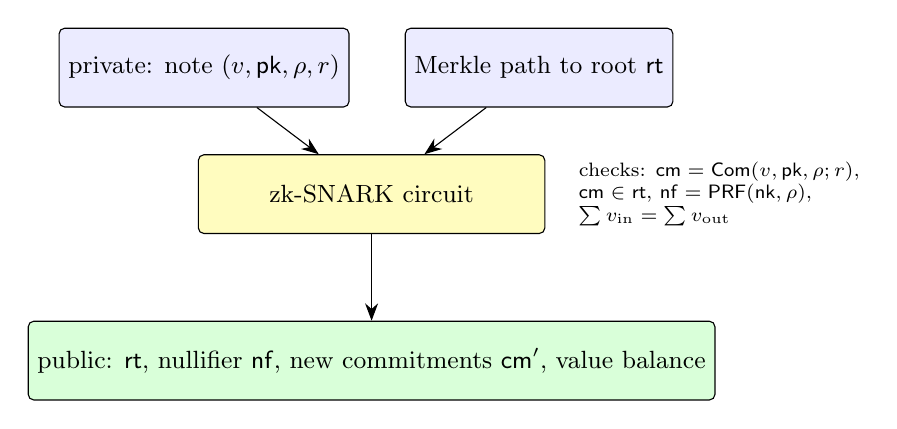
\begin{tikzpicture}[node distance=0.9cm and 0.7cm]
\node[blk,minimum width=2.6cm] (n) {private: note $(v,\mathsf{pk},\rho,r)$};
\node[blk,minimum width=2.6cm,right=of n] (p) {Merkle path to root $\mathsf{rt}$};
\node[blk,fill=yellow!25,below=1.1cm of $(n)!0.5!(p)$,minimum width=4.4cm] (c) {zk-SNARK circuit};
\node[blk,fill=green!15,below=1.1cm of c,minimum width=7.4cm] (o) {public: $\mathsf{rt}$, nullifier $\mathsf{nf}$, new commitments $\mathsf{cm}'$, value balance};
\draw[->] (n)--(c); \draw[->] (p)--(c); \draw[->] (c)--(o);
\node[right=0.3cm of c,font=\scriptsize,align=left] {checks: $\mathsf{cm}=\mathsf{Com}(v,\mathsf{pk},\rho;r)$,\\ $\mathsf{cm}\in\mathsf{rt}$, $\mathsf{nf}=\mathsf{PRF}(\mathsf{nk},\rho)$,\\ $\sum v_{\text{in}}=\sum v_{\text{out}}$};
\end{tikzpicture}
\caption{Zcash shielded spend: the proof hides the note and the Merkle path; the chain sees only $\mathsf{rt}$, the nullifier and fresh commitments.}
\end{figure}

\begin{center}\small
\begin{tabular}{@{}llll@{}}
\toprule
\textbf{Hidden} & \textbf{Monero} & \textbf{Zcash (shielded)} & \textbf{Bitcoin}\\
\midrule
Sender & ring signature with decoys & zk-SNARK (membership in the note tree) & public\\
Receiver & one-time stealth address & encrypted note & public address\\
Amount & Pedersen commitment + range proof & inside the proof & public\\
\bottomrule
\end{tabular}
\end{center}

\subsection{zk-rollups}

\begin{plainenglish}
Blockchains are slow because every node re-executes every transaction. A \textbf{zk-rollup} executes thousands of transactions off-chain, then posts to the chain only the new state root plus one short proof that ``these transactions were valid and take state $S$ to state $S'$''. The chain verifies a single small proof instead of re-running the batch. Here zero knowledge is mostly used for \emph{succinctness}, not privacy.
\end{plainenglish}

\begin{exbox}[rollup arithmetic]
A batch of $5000$ transfers costs $21{,}000$ gas each on layer~1: $1.05\times10^8$ gas. A rollup posts compressed data and one proof, say $\approx5\times10^5$ gas for verification plus data, a reduction by about two orders of magnitude (the exact factor depends on the data-availability scheme and proof system).
\end{exbox}

\begin{exercisebox}
\begin{enumerate}[nosep]
\item Check Example~\ref{ex:pedersen} for the commitment $\mathsf{Com}(2;3)\cdot\mathsf{Com}(5;1)$.
\item Explain why a Pedersen commitment cannot be both perfectly hiding and perfectly binding.
\item Flatten $y=x^2+3x+2$ into R1CS and give the witness for $x=4$.
\item In a ring of size $r$, what is the probability that a random decoy selection includes the real spender's output if decoys are picked uniformly from $N$ outputs? Discuss why age-biased selection matters.
\item Why does the nullifier have to be deterministic given the note but unlinkable to the note's commitment?
\end{enumerate}
\end{exercisebox}
%================================================================
\section{Advanced Topics}\label{sec:advanced}
%================================================================

\subsection{BLS signatures and aggregation}

\begin{plainenglish}
Ethereum's proof-of-stake has hundreds of thousands of validators that all vote on every block. Storing and checking that many signatures is too expensive. \textbf{BLS signatures}~\cite{BLS01} have a remarkable property: you can
\emph{add up} many signatures into a single short signature, and one check verifies them all. Two-thirds of the validators can thus be represented by one 96-byte signature plus a bit-field saying who signed.
\end{plainenglish}

\begin{formal}
Let $e:\G_1\times\G_2\to\G_T$ be a bilinear pairing ($e(g_1^a,g_2^b)=e(g_1,g_2)^{ab}$) with generators $g_1,g_2$ and $\Hash:\{0,1\}^*\to\G_2$ (a hash-to-curve function). Following Ethereum's BLS12-381 convention, public keys live in $\G_1$ ($48$ bytes) and signatures in $\G_2$ ($96$ bytes).
\begin{itemize}[nosep]
\item $\KeyGen$: $x\leftarrow_\$\Z_q$, $\pk=g_1^x$. \quad $\Sign$: $\sigma=\Hash(m)^x$. \quad $\Verify$: accept iff $e(g_1,\sigma)=e(\pk,\Hash(m))$.
\end{itemize}
Correctness: $e(g_1,\Hash(m)^x)=e(g_1,\Hash(m))^x=e(g_1^x,\Hash(m))$.

\begin{proposition}[Aggregation on a common message]
Given signatures $\sigma_i=\Hash(m)^{x_i}$ on the same $m$, let $\sigma=\prod\sigma_i$ and $\pk=\prod\pk_i$. Then $\sigma=\Hash(m)^{\sum x_i}$ and $e(g_1,\sigma)=e(\pk,\Hash(m))$. 
\end{proposition}
\begin{warnbox}[(rogue-key attack)]
Mallory registers $\pk_M=g_1^{y}\cdot(\pk_{\text{Alice}})^{-1}$ without knowing its secret key. The aggregate key $\pk_A\pk_M=g_1^y$ is one she controls: she can forge a ``joint'' signature on behalf of both. Defence: require a \emph{proof of possession} (a signature on one's own public key) at registration.
\end{warnbox}
\end{formal}

\begin{exbox}[savings]
$10{,}000$ validators sign a block. Individual signatures: $10{,}000\times96$ B $\approx960$ kB. Aggregate: $96$ B plus a $10{,}000$-bit mask ($1250$ B). Verification requires \emph{two pairings} and $10{,}000$ group additions, instead of $10{,}000$ pairing checks.
\end{exbox}

\subsection{Threshold signatures and secret sharing}

\begin{plainenglish}
Instead of one person holding a key, split it among $n$ people so that any $t$ of them can sign together but $t-1$ learn nothing. Wallets for exchanges and bridges use this so that no single stolen device means stolen funds.
\textbf{Shamir's secret sharing} does the splitting: a secret is the height at which a hidden line (or curve) crosses the vertical axis; each share is one point on it. Two points determine a line; one point tells you nothing.
\end{plainenglish}

\begin{formal}
\begin{theorem}[Shamir~\cite{Sha79}]
Let $\F_p$ be a prime field, $s\in\F_p$, and $f(X)=s+a_1X+\dots+a_{t-1}X^{t-1}$ with $a_i\leftarrow_\$\F_p$. Share $i$ is $(i,f(i))$. Any $t$ shares recover $s=\sum_{i\in S}\lambda_if(i)$ with Lagrange coefficients $\lambda_i=\prod_{j\in S,j\ne i}\frac{j}{j-i}$.
Any $t-1$ shares are uniformly distributed, \ie\ perfectly hide $s$.
\end{theorem}
\begin{proof}
Recovery: $f$ has degree $<t$ and is determined by $t$ points via Lagrange interpolation; evaluate at $0$. Hiding: for any candidate secret $s'$ and any $t-1$ shares at nonzero points, there is exactly one polynomial of degree $<t$ through $(0,s')$ and the $t-1$ points, and each corresponds to the same number of random choices of $(a_1,\dots,a_{t-1})$, so the shares are independent of $s$.
\end{proof}
For BLS (and Schnorr) the signing key $x=f(0)$ stays shared: each party signs with its share $x_i=f(i)$ and the partial signatures are combined \emph{in the exponent} by the same Lagrange coefficients: $\sigma=\prod_{i\in S}\sigma_i^{\lambda_i}=\Hash(m)^{x}$.
\end{formal}

\begin{exbox}[$t=2$, $n=3$ over $\F_{11}$]\label{ex:shamir}
Secret $s=7$, random slope $a_1=3$: $f(X)=7+3X$. Shares: $f(1)=10$, $f(2)=13\equiv2$, $f(3)=16\equiv5$. Recover from parties $1$ and $2$: $\lambda_1=\frac{2}{2-1}=2$, $\lambda_2=\frac{1}{1-2}=-1$, so $s=2\cdot10-2=18\equiv7$ \checkmark. Recover from $1$ and $3$: $\lambda_1=\frac{3}{3-1}=3/2=3\cdot6=18\equiv7$ (since $2^{-1}=6$), $\lambda_3=\frac{1}{1-3}=-1/2=-6\equiv5$; $s=7\cdot10+5\cdot5=95\equiv7$ \checkmark.
\end{exbox}

\begin{figure}[htbp]
\centering
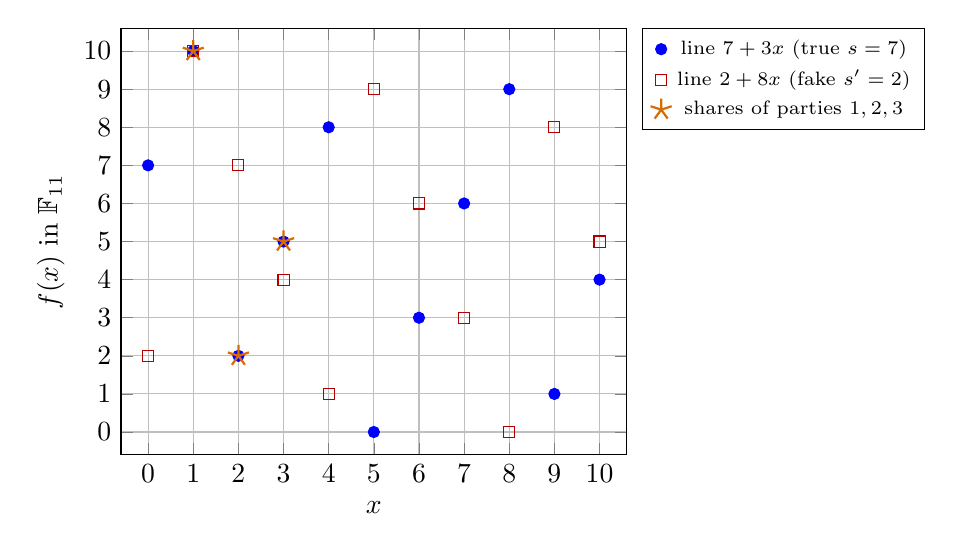
\begin{tikzpicture}
\begin{axis}[width=0.66\textwidth,height=7cm,xmin=-0.6,xmax=10.6,ymin=-0.6,ymax=10.6,xtick={0,...,10},ytick={0,...,10},grid=both,
 xlabel={$x$},ylabel={$f(x)$ in $\F_{11}$},legend style={at={(1.03,1)},anchor=north west,font=\scriptsize},mark size=2pt]
\addplot[only marks,mark=*,blue] coordinates {(0,7) (1,10) (2,2) (3,5) (4,8) (5,0) (6,3) (7,6) (8,9) (9,1) (10,4)};
\addlegendentry{line $7+3x$ (true $s=7$)}
\addplot[only marks,mark=square,red!70!black] coordinates {(0,2) (1,10) (2,7) (3,4) (4,1) (5,9) (6,6) (7,3) (8,0) (9,8) (10,5)};
\addlegendentry{line $2+8x$ (fake $s'=2$)}
\addplot[only marks,mark=star,mark size=4pt,orange!85!black,thick] coordinates {(1,10) (2,2) (3,5)};
\addlegendentry{shares of parties $1,2,3$}
\end{axis}
\end{tikzpicture}
\caption{Shamir sharing with $t=2$ over $\F_{11}$ (Example~\ref{ex:shamir}). Over a finite field a ``line'' is a set of $11$ points. Share~$1$, the point $(1,10)$, lies on a line through \emph{every} possible intercept (the red line is one of them), so a single share reveals nothing; two shares determine the line and hence $f(0)=7$.}
\end{figure}

\subsection{Verifiable delay functions (VDFs)}

\begin{plainenglish}
Some applications need a number that nobody can predict \emph{in advance} and that nobody can speed up with more machines, such as an unbiasable lottery for choosing block producers. A \textbf{VDF}~\cite{BBBF18} is a function that takes a prescribed number of \emph{sequential} steps to compute (say, ten minutes), no matter how many processors you have,
but whose output can be verified quickly. Like boiling an egg: nine women cannot boil an egg in one minute.
\end{plainenglish}

\begin{formal}
\textbf{Repeated squaring.} Let $N=pq$ be an RSA modulus of unknown factorisation. Define $y=x^{2^T}\bmod N$. Computing $y$ takes $T$ squarings, which are believed inherently sequential. Whoever knows $\varphi(N)$ computes it in $O(\log N)$ time by reducing $2^T$ modulo $\varphi(N)$, hence the unknown order requirement.
\emph{Wesolowski's proof}~\cite{Wes19}: the verifier sends a random prime $\ell$; the prover returns $\pi=x^{\lfloor2^T/\ell\rfloor}$; the verifier computes $r=2^T\bmod\ell$ and checks $\pi^\ell x^r=y$. Correctness: $2^T=\ell\lfloor2^T/\ell\rfloor+r$.
\end{formal}

\begin{exbox}[tiny VDF]\label{ex:vdf}
$N=35$, $x=2$, $T=3$: $y=2^{8}=256\equiv11\pmod{35}$ (by squaring three times: $2\to4\to16\to256\equiv11$). Verify with $\ell=3$: $\lfloor8/3\rfloor=2$, $r=8\bmod3=2$, $\pi=2^2=4$. Check: $\pi^\ell x^r=4^3\cdot2^2=64\cdot4=256\equiv11$ \checkmark.
\end{exbox}

\begin{figure}[htbp]
\centering
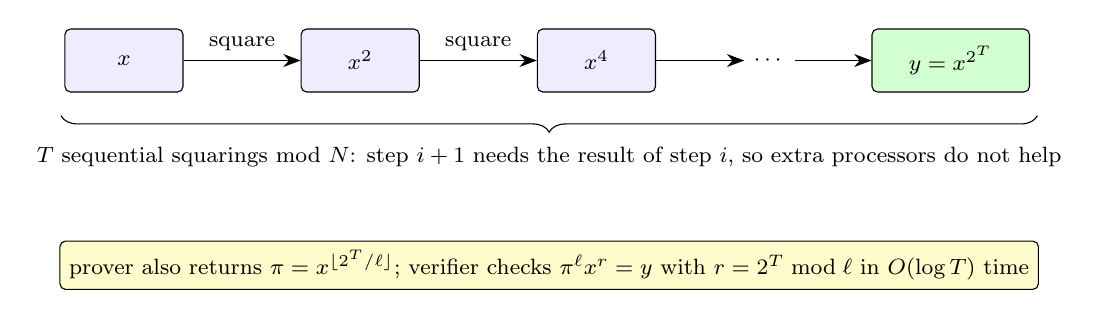
\begin{tikzpicture}[font=\footnotesize,
 b/.style={draw,rounded corners=2pt,minimum width=1.5cm,minimum height=0.8cm,fill=blue!7}]
\node[b] (x0) at (0,0) {$x$};
\node[b] (x1) at (3,0) {$x^2$};
\node[b] (x2) at (6,0) {$x^4$};
\node (d) at (8.2,0) {$\cdots$};
\node[b,fill=green!18,minimum width=2cm] (y) at (10.5,0) {$y=x^{2^T}$};
\draw[->] (x0)--node[above]{square}(x1); \draw[->] (x1)--node[above]{square}(x2); \draw[->] (x2)--(d); \draw[->] (d)--(y);
\draw[decorate,decoration={brace,mirror,amplitude=6pt}] (-0.8,-0.7) -- (11.6,-0.7) node[midway,below=8pt] {$T$ sequential squarings mod $N$: step $i+1$ needs the result of step $i$, so extra processors do not help};
\node[draw,rounded corners=2pt,fill=yellow!20,align=center] at (5.4,-2.6) {prover also returns $\pi=x^{\lfloor 2^T/\ell\rfloor}$; verifier checks $\pi^{\ell}x^{r}=y$ with $r=2^T\bmod\ell$ in $O(\log T)$ time};
\end{tikzpicture}
\caption{A verifiable delay function from repeated squaring in a group of unknown order, with Wesolowski's proof.}
\end{figure}

\subsection{MEV: miner (maximal) extractable value}

\begin{plainenglish}
The block producer decides the \emph{order} of transactions in a block, and ordering has monetary value. Specialised bots (``searchers'') watch the public queue of pending transactions and pay to be ordered before or after them: this is \textbf{MEV}~\cite{DGKLZBBJ20}. A classic example is the \textbf{sandwich attack} on a decentralised exchange:
the bot buys just before your trade (pushing the price up), lets your trade execute at the worse price, then sells right after for a profit. You lose; the bot and the block producer split the spoils. MEV is a consensus-level security problem: it creates incentives to reorder or even reorganise blocks.
\end{plainenglish}

\begin{formal}
\textbf{Constant-product AMM.} A pool holding $x$ units of ETH and $y$ of USDC keeps $xy=k$ (ignoring fees). Buying with $\Delta y$ USDC gives $\Delta x=x-\dfrac{k}{y+\Delta y}$ ETH.
\end{formal}

\begin{exbox}[a sandwich with numbers, no fees]\label{ex:sandwich}
Pool: $x=1000$ ETH, $y=2{,}000{,}000$ USDC (price $2000$). A user wants to buy ETH with $400{,}000$ USDC.
\begin{itemize}[nosep]
\item \emph{Alone}: $\Delta x=1000-\frac{2\cdot10^9}{2.4\cdot10^6}=166.67$ ETH (average price $2400$).
\item \emph{Attacker front-runs} with $200{,}000$ USDC: receives $90.91$ ETH; pool becomes $909.09$ ETH, $2.2$M USDC.
\item \emph{User} (same $400{,}000$ USDC) now gets $139.86$ ETH (average price $2860$): a loss of $26.8$ ETH.
\item \emph{Attacker back-runs}: sells $90.91$ ETH and receives $274{,}797$ USDC, a profit of about $74{,}800$ USDC.
\end{itemize}
Defence: a tight slippage limit makes the victim's trade revert, private order flow, and batch auctions or commit--reveal ordering.
\end{exbox}

\begin{figure}[htbp]
\centering
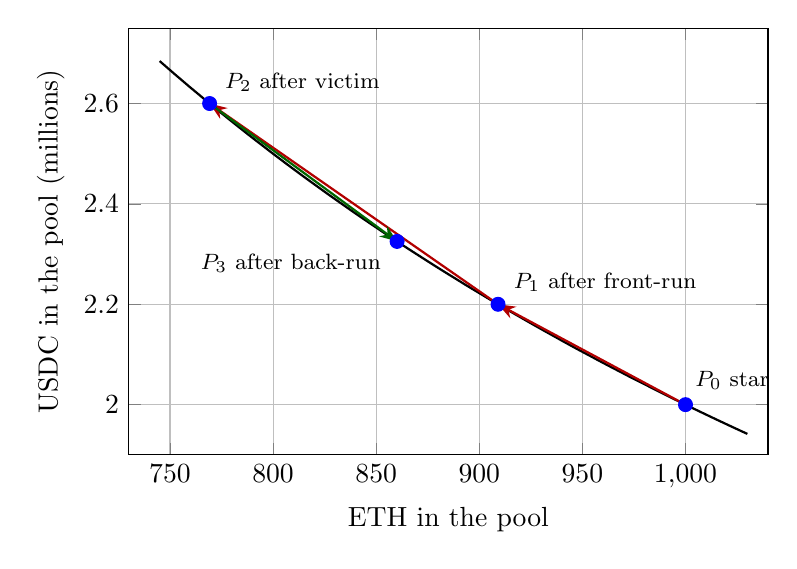
\begin{tikzpicture}
\begin{axis}[width=0.8\textwidth,height=7cm,xlabel={ETH in the pool},ylabel={USDC in the pool (millions)},
 xmin=730,xmax=1040,ymin=1.9,ymax=2.75,grid=both,xtick={750,800,...,1000},ytick={2,2.2,2.4,2.6}]
\addplot[black,thick,domain=745:1030,samples=80] {2000/x};
\addplot[only marks,mark=*,mark size=2.5pt,blue] coordinates {(1000,2.0) (909.09,2.2) (769.23,2.6) (860.14,2.3252)};
\node[font=\footnotesize,anchor=south west] at (axis cs:1000,2.01) {$P_0$ start};
\node[font=\footnotesize,anchor=south west] at (axis cs:912,2.205) {$P_1$ after front-run};
\node[font=\footnotesize,anchor=south west] at (axis cs:772,2.605) {$P_2$ after victim};
\node[font=\footnotesize,anchor=north east] at (axis cs:857,2.32) {$P_3$ after back-run};
\draw[->,red!70!black,thick] (axis cs:1000,2.0)--(axis cs:909.09,2.2);
\draw[->,red!70!black,thick] (axis cs:909.09,2.2)--(axis cs:769.23,2.6);
\draw[->,green!40!black,thick] (axis cs:769.23,2.6)--(axis cs:860.14,2.3252);
\end{axis}
\end{tikzpicture}
\caption{The sandwich of Example~\ref{ex:sandwich} on the curve $xy=k$ (no fees). The bot pushes the price up with the front-run, the victim trades at the worse price, and the bot sells back down the curve for a profit.}
\end{figure}

\subsection{Quantum computers}

\begin{plainenglish}
\textbf{Shor's algorithm}~\cite{Sho94} would break the discrete logarithm problem, and with it ECDSA and Schnorr: a quantum attacker could compute your secret key from your public key. Coins whose public key is already visible on chain (any address that has been spent from, or old pay-to-public-key outputs) are at risk;
coins behind a never-spent hash address are protected by the hash until the owner reveals the key. \textbf{Grover's algorithm} speeds up brute-force search quadratically, so SHA-256 preimage resistance drops from $2^{256}$ to roughly $2^{128}$ quantum steps and mining speeds up at most quadratically in theory, but Grover does not parallelise well,
so it is considered a much smaller threat than Shor. The response is migration to \textbf{post-quantum signatures}: hash-based (XMSS; SLH-DSA, the standardised SPHINCS+) and lattice-based (ML-DSA, the standardised Dilithium) schemes, standardised by NIST in 2024~\cite{NIST24}, at the cost of larger signatures (kilobytes instead of $64$ bytes).
\end{plainenglish}

\begin{exbox}[size cost]
A Bitcoin block of $1$ MB fits roughly $4000$ transactions with $64$-byte Schnorr signatures. With Dilithium2 (ML-DSA-44), whose signatures take $2420$ bytes and whose public keys take $1312$ bytes, the signature alone is $\approx38\times$ and the key $\approx41\times$ larger than with Schnorr, so far fewer transactions fit unless the block size or the aggregation technology changes.
\end{exbox}

\begin{exercisebox}
\begin{enumerate}[nosep]
\item Prove the BLS aggregate verification equation for signatures on \emph{different} messages: $e(g_1,\prod\sigma_i)=\prod e(\pk_i,\Hash(m_i))$.
\item Share secret $s=4$ in a $(2,4)$ scheme over $\F_{13}$ with slope $a_1=5$ and reconstruct from shares $2$ and $4$.
\item Redo Example~\ref{ex:sandwich} with a front-run of $100{,}000$ USDC. Does the attacker's profit increase or decrease? Why?
\item Show that in the repeated squaring VDF, knowledge of $\varphi(N)$ breaks the sequentiality.
\item Estimate the Grover cost to find a SHA-256 preimage on a quantum computer with $10^9$ evaluations per second.
\end{enumerate}
\end{exercisebox}

%================================================================
\section{Open Problems and Wrap-up}\label{sec:open}
%================================================================

\begin{plainenglish}
Hashes and signatures are the glue of a blockchain, proof of work (or stake) is its Sybil defence, and the longest-chain rule together with an honest majority yields probabilistic agreement. Several questions remain open.
\end{plainenglish}

\begin{itemize}
\item \textbf{The scalability trilemma.} It is hard to get decentralisation, security and throughput all at once. Sharding, rollups, DAG-based protocols (Narwhal--Bullshark) and data-availability sampling are the main attempts.
\item \textbf{Provable security of PoS in the permissionless setting.} Dynamic availability and finality cannot coexist under partial synchrony (the \emph{availability-finality dilemma}), motivating hybrid designs such as ebb-and-flow protocols~\cite{Neu21}, which Ethereum's Gasper resembles.
\item \textbf{Incentive-compatibility.} Selfish mining and MEV show that honest behaviour is not always an equilibrium. Characterising incentive-compatible protocols is open.
\item \textbf{Efficient post-quantum primitives} with small signatures and good aggregation.
\item \textbf{Privacy versus regulation}, including selective disclosure and auditable privacy.
\item \textbf{Efficient transparent proofs}: SNARKs without trusted setup that are fast to prove and tiny to verify.
\item \textbf{Cross-chain security}: bridges have lost billions of dollars; light-client based bridges and formally verified bridge contracts are a major research area.
\end{itemize}

\begin{exercisebox}
Project ideas: (a) simulate the double-spend success probability and compare with Nakamoto and with the exact negative-binomial value; (b) implement the Eyal--Sirer Markov chain and reproduce the threshold plot; (c) implement Schnorr, Shamir and a simple Merkle tree in Python; (d) write a security analysis of a recent bridge exploit.
\end{exercisebox}


\newpage
\section*{Appendix: Hints and Answers to Selected Exercises}
\addcontentsline{toc}{section}{Appendix: Hints and Answers to Selected Exercises}
\small
All numerical answers were checked by computer.

\paragraph{Part 1.}
\begin{enumerate}[nosep,leftmargin=1.5em]
\item A signature proves authorship of one message; it says nothing about the order of two messages or about other messages signed with the same key. Both $m_1$ and $m_2$ verify, so recipients cannot tell which payment is valid.
\item Identities cost nothing, so an attacker creates as many as she likes and out-votes everyone.
\item For $k=0$ the finalized ledger is the whole chain, so every ordinary fork (which Nakamoto consensus cannot avoid) violates persistence with non-negligible probability. A larger $k$ makes violations exponentially unlikely, but a merchant waits $k$ block intervals and the liveness parameter $u$ grows with $k$.
\end{enumerate}

\paragraph{Part 2.}
\begin{enumerate}[nosep,leftmargin=1.5em]
\item $q\approx1.18\cdot2^{32}\approx5.1\times10^{9}$ evaluations.
\item The lists $[a,b,c]$ and $[a,b,c,c]$ have the same root (Figure~\ref{fig:merkledup}). Avoid the ambiguity by promoting the odd node unchanged, or by hashing the number of leaves into the root.
\item $y=4^4=3$, $R=4^2=16$, $s=2+9\cdot4=38\equiv5\pmod{11}$. Check: $g^s=4^5=12$ and $R\,y^c=16\cdot3^9=16\cdot18=288\equiv12\pmod{23}$.
\item $s_1-s_2=(c_1-c_2)x$, so $x=(s_1-s_2)(c_1-c_2)^{-1}\bmod q$; the inverse exists unless $c_1=c_2$, \ie\ a hash collision.
\item Given a second-preimage finder $\Adv'$, a collision finder samples $x$, runs $\Adv'(x)$ to get $x'$ and outputs $(x,x')$.
\item $\sigma(7)=7^{27}\bmod55=28$ and $28^3\equiv7$. With $\sigma(12)=23$: $28\cdot23=644\equiv39$ and $39^3\equiv29=84\bmod55$.
\item $\sigma(h_1)\sigma(h_2)^{-1}=h_1^d(h_2^{d})^{-1}=(h_1h_2^{-1})^d$.
\end{enumerate}

\paragraph{Part 3.}
\begin{enumerate}[nosep,leftmargin=1.5em]
\item Inputs $15.7$, outputs $15.7$: valid with fee $0$ (many nodes would refuse to relay it).
\item An attacker could mine many blocks at very low difficulty and obtain a longer chain with far less total work.
\item Each of the $m$ blocks is found by the miner independently with probability $\alpha$ (Corollary), so the count is $\mathrm{Bin}(m,\alpha)$.
\item $T_{\text{new}}/T_{\text{old}}=20/14\approx1.43$ (easier).
\item $1.2\times10^{23}$ hashes per block, $\log_2\approx76.7$, so about $77$ leading zero bits.
\end{enumerate}

\paragraph{Part 4.}
\begin{enumerate}[nosep,leftmargin=1.5em]
\item $(2/3)^3=8/27\approx0.296$.
\item $P_{\text{Nak}}(0.25,4)\approx0.1235$ (the exact value is $0.1411$).
\item $1-\sum_{k\le z}\Pr[K=k]\big(1-(q/p)^{z-k}\big)=\Pr[K>z]+\sum_{k\le z}\Pr[K=k](q/p)^{z-k}$.
\item $R_{\text{pool}}=0.1808/0.344\approx0.526>0.4$: profitable.
\item Delay wastes honest work: fewer rounds are convergence opportunities, $\alpha(1-2(\Delta+1)\alpha)$ shrinks, and the adversary needs a smaller relative share to satisfy $\beta\ge\alpha(1-2(\Delta+1)\alpha)$.
\end{enumerate}

\paragraph{Part 5.}
\begin{enumerate}[nosep,leftmargin=1.5em]
\item $f=3$, quorum $7$, overlap $\ge2\cdot7-10=4=f+1$, so at least one honest replica.
\item $|Q_1\cap Q_2|\ge2\lceil\frac{n+f+1}2\rceil-n\ge f+1$. For $n=3f+1$ the size is $2f+1$.
\item With signatures the traitor cannot make $B$ believe ``$A$ said $X$'' without $A$'s signature, so the hexagon simulation fails. In the synchronous model, Dolev--Strong~\cite{DS83} gives Byzantine broadcast for any $f<n$ (in $f+1$ rounds), and agreement with validity for $f<n/2$.
\item Without slashing, voting on both branches costs nothing and earns the reward on whichever branch wins; voting on one branch earns only if it wins.
\item $(1-f_{\text{act}})^{\sigma_1}(1-f_{\text{act}})^{\sigma_2}=(1-f_{\text{act}})^{\sigma_1+\sigma_2}$ by the exponent rule, so splitting stake leaves the probability $1-(1-f_{\text{act}})^{\sigma_1+\sigma_2}$ unchanged.
\end{enumerate}

\paragraph{Part 6.}
\begin{enumerate}[nosep,leftmargin=1.5em]
\item Checks--effects--interactions:
\begin{lstlisting}[language=Solidity]
function withdraw() public {
    uint amount = balance[msg.sender];
    balance[msg.sender] = 0;                          // effect first
    (bool ok, ) = msg.sender.call{value: amount}("");  // interaction last
    require(ok);
}
\end{lstlisting}
\item $10\cdot1.125^3\approx14.24$ gwei.
\item $\sum_a\texttt{balanceOf}[a]=\texttt{totalSupply}$. A mint or burn that updates only one side, or a transfer with unchecked arithmetic, violates it.
\item All nodes must compute the same state. Controlled sources: time (only the agreed block timestamp), randomness (no true random source; block-derived values are biasable), external data (no network or file access; oracles deliver data inside transactions). Floating point is also excluded.
\end{enumerate}

\paragraph{Part 7.}
\begin{enumerate}[nosep,leftmargin=1.5em]
\item $\mathsf{Com}(2;3)=3$, $\mathsf{Com}(5;1)=16$, product $48\equiv2$, and $\mathsf{Com}(7;4)=4^7\cdot9^4=8\cdot6=48\equiv2$ \checkmark.
\item Perfect hiding means every commitment opens to every message (for suitable randomness), so it is not binding against unbounded adversaries. Perfect binding fixes the message, so an unbounded adversary can read it.
\item $w_1=x\cdot x$ and $(w_1+3x+2)\cdot1=y$. Witness $(1,y,x,w_1)=(1,30,4,16)$.
\item The real output is in the ring by construction; any \emph{given} other output is chosen as a decoy with probability $(r-1)/(N-1)$. Real spends are biased towards young outputs, so uniform decoys are older than the real input and the youngest ring member is likely the signer; decoys should imitate the spending-age distribution.
\item Determinism makes a second spend produce the same nullifier, which is detected. It is derived with a secret key through a PRF, so nobody can link it to the note's commitment.
\end{enumerate}

\paragraph{Part 8.}
\begin{enumerate}[nosep,leftmargin=1.5em]
\item $e(g_1,\prod\sigma_i)=\prod e(g_1,\Hash(m_i)^{x_i})=\prod e(g_1^{x_i},\Hash(m_i))=\prod e(\pk_i,\Hash(m_i))$.
\item $f(X)=4+5X$, $f(2)=1$, $f(4)=11$, $\lambda_2=2$, $\lambda_4=-1$, $s=2\cdot1-11=-9\equiv4$ \checkmark.
\item The bot gets $47.62$ ETH, the victim $152.38$ ETH (loss $14.29$ ETH), and the bot's profit falls to about $40{,}449$ USDC. Profit comes from the price impact imposed on the victim, which grows with the size of the front-run (until the victim's slippage limit makes the trade revert).
\item With $\varphi(N)$, compute $2^T\bmod\varphi(N)$ and do one modular exponentiation in $O(\log N)$ time; no sequential delay remains.
\item Grover needs about $2^{128}$ sequential evaluations: $2^{128}/10^9\approx3.4\times10^{29}$ s $\approx10^{22}$ years.
\end{enumerate}
\normalsize

\begin{thebibliography}{99}
\bibitem{Nak08} S.~Nakamoto. \emph{Bitcoin: A Peer-to-Peer Electronic Cash System}, 2008.
\bibitem{GKL15} J.~Garay, A.~Kiayias, N.~Leonardos. The Bitcoin Backbone Protocol: Analysis and Applications. \emph{EUROCRYPT 2015}.
\bibitem{PSS17} R.~Pass, L.~Seeman, a.~shelat. Analysis of the Blockchain Protocol in Asynchronous Networks. \emph{EUROCRYPT 2017}.
\bibitem{ES14} I.~Eyal, E.~G.~Sirer. Majority is not Enough: Bitcoin Mining is Vulnerable. \emph{Financial Cryptography 2014}.
\bibitem{Ros14} M.~Rosenfeld. Analysis of Hashrate-Based Double Spending. arXiv:1402.2009, 2014.
\bibitem{GP18} C.~Grunspan, R.~P\'erez-Marco. Double spend races. \emph{Int.\ J.\ Theoretical and Applied Finance}, 2018.
\bibitem{LSP82} L.~Lamport, R.~Shostak, M.~Pease. The Byzantine Generals Problem. \emph{ACM TOPLAS}, 1982.
\bibitem{FLP85} M.~Fischer, N.~Lynch, M.~Paterson. Impossibility of Distributed Consensus with One Faulty Process. \emph{J.\ ACM}, 1985.
\bibitem{DLS88} C.~Dwork, N.~Lynch, L.~Stockmeyer. Consensus in the Presence of Partial Synchrony. \emph{J.\ ACM}, 1988.
\bibitem{CL99} M.~Castro, B.~Liskov. Practical Byzantine Fault Tolerance. \emph{OSDI 1999}.
\bibitem{KRDO17} A.~Kiayias, A.~Russell, B.~David, R.~Oliynykov. Ouroboros: A Provably Secure Proof-of-Stake Blockchain Protocol. \emph{CRYPTO 2017}.
\bibitem{BG17} V.~Buterin, V.~Griffith. Casper the Friendly Finality Gadget. arXiv:1710.09437, 2017.
\bibitem{Woo14} G.~Wood. \emph{Ethereum: A Secure Decentralised Generalised Transaction Ledger} (Yellow Paper).
\bibitem{PS96} D.~Pointcheval, J.~Stern. Security Proofs for Signature Schemes. \emph{EUROCRYPT 1996}.
\bibitem{Ped91} T.~P.~Pedersen. Non-Interactive and Information-Theoretic Secure Verifiable Secret Sharing. \emph{CRYPTO 1991}.
\bibitem{BCGGMTV14} E.~Ben-Sasson et al. Zerocash: Decentralized Anonymous Payments from Bitcoin. \emph{IEEE S\&P 2014}.
\bibitem{Gro16} J.~Groth. On the Size of Pairing-based Non-interactive Arguments. \emph{EUROCRYPT 2016}.
\bibitem{BLS01} D.~Boneh, B.~Lynn, H.~Shacham. Short Signatures from the Weil Pairing. \emph{ASIACRYPT 2001}.
\bibitem{Sha79} A.~Shamir. How to Share a Secret. \emph{Commun.\ ACM}, 1979.
\bibitem{BBBF18} D.~Boneh, J.~Bonneau, B.~B\"unz, B.~Fisch. Verifiable Delay Functions. \emph{CRYPTO 2018}.
\bibitem{Wes19} B.~Wesolowski. Efficient Verifiable Delay Functions. \emph{EUROCRYPT 2019}.
\bibitem{DGKLZBBJ20} P.~Daian et al. Flash Boys 2.0: Frontrunning in Decentralized Exchanges, Miner Extractable Value, and Consensus Instability. \emph{IEEE S\&P 2020}.
\bibitem{BMRS16} B.~B\"unz et al. Bulletproofs: Short Proofs for Confidential Transactions and More. \emph{IEEE S\&P 2018}.
\bibitem{Sho94} P.~Shor. Algorithms for Quantum Computation: Discrete Logarithms and Factoring. \emph{FOCS 1994}.
\bibitem{BMC15} A.~Narayanan, J.~Bonneau, E.~Felten, A.~Miller, S.~Goldfeder. \emph{Bitcoin and Cryptocurrency Technologies}. Princeton University Press, 2016.
\bibitem{PSL80} M.~Pease, R.~Shostak, L.~Lamport. Reaching Agreement in the Presence of Faults. \emph{J.\ ACM}, 1980.
\bibitem{DS83} D.~Dolev, H.~R.~Strong. Authenticated Algorithms for Byzantine Agreement. \emph{SIAM J.\ Computing}, 1983.
\bibitem{BR93} M.~Bellare, P.~Rogaway. Random Oracles are Practical. \emph{ACM CCS 1993}.
\bibitem{Coron00} J.-S.~Coron. On the Exact Security of Full Domain Hash. \emph{CRYPTO 2000}.
\bibitem{Neu21} J.~Neu, E.~N.~Tas, D.~Tse. Ebb-and-Flow Protocols: A Resolution of the Availability-Finality Dilemma. \emph{IEEE S\&P 2021}.
\bibitem{NIST24} NIST. FIPS 203 (ML-KEM), FIPS 204 (ML-DSA), FIPS 205 (SLH-DSA), 2024.
\bibitem{EIP1559} V.~Buterin et al. EIP-1559: Fee market change for ETH~1.0 chain, 2019.
\bibitem{BIP340} P.~Wuille, J.~Nick, T.~Ruffing. BIP-340: Schnorr Signatures for secp256k1, 2020.
\end{thebibliography}

\end{document}
